%% Dexterous Manipulation, Single-Hand and Bimanual: a survey.
%% IEEEtran journal class, two columns, as used by robotics surveys posted to arXiv.
%% Build:  latexmk -pdf main.tex     (see tools/build_tex.sh)
\documentclass[journal,twoside]{IEEEtran}
% --- classes and fonts -------------------------------------------------------
\usepackage[T1]{fontenc}
\usepackage[utf8]{inputenc}
\usepackage{microtype}
\usepackage{amsmath,amssymb}
\usepackage{graphicx}
\usepackage[table]{xcolor}
\usepackage{booktabs}
\usepackage{multirow}
\usepackage{array}
\usepackage{tabularx}
\usepackage{longtable}
\usepackage{caption}
\usepackage{subcaption}
\usepackage{tikz}
\usepackage{url}
\usepackage[hidelinks,breaklinks]{hyperref}
\usepackage{balance}

% --- the restrained palette --------------------------------------------------
% One muted accent and greyscale. No gradients, no fills beyond a light wash.
\definecolor{accent}{HTML}{2F5D7C}
\definecolor{wash}{HTML}{F2F4F6}
\definecolor{rule}{HTML}{B9C2C9}
\definecolor{warn}{HTML}{8C4A32}

% --- table style -------------------------------------------------------------
\renewcommand{\arraystretch}{1.12}
\setlength{\tabcolsep}{4pt}
\newcolumntype{L}[1]{>{\raggedright\arraybackslash}p{#1}}
\newcolumntype{C}[1]{>{\centering\arraybackslash}p{#1}}
\newcommand{\hdr}[1]{\textbf{#1}}
\newcommand{\na}{\textcolor{black!35}{--}}   % a value no source stated

% --- citation keys shown inline ---------------------------------------------
\newcommand{\key}[1]{\texttt{\small #1}}

% --- captions ----------------------------------------------------------------
\captionsetup{font=small,labelfont=bf,skip=4pt}
\captionsetup[table]{position=top,skip=3pt}
\captionsetup[sub]{font=small}

% --- reproduced-figure credit line ------------------------------------------
% Every reproduced figure states where it came from, under the caption.
\newcommand{\credit}[1]{\par\vspace{1pt}{\scriptsize\textcolor{black!55}{Reproduced from #1.}}}
% A reproduced figure states its source and, until permission is recorded, says so quietly.
\newcommand{\pending}[1]{\par\vspace{1pt}{\scriptsize\textcolor{black!50}{\textit{Reproduced from} #1\textit{; permission not yet sought, see the register.}}}}

% The one reproduced plate.
% Rebuilt from its source PDF by tools/relayout_plates.py; see tex/figs/SELECTED.md for the crop
% box and tex/PERMISSIONS.md for the licence it is used under.
%
% A plate is kept only where a photograph or a render carries something a drawing cannot, and
% only where the paper has the right to print it without asking anyone. Everything else that was
% reproduced has been redrawn in the paper's own style (figs/fig_transmission, fig_collision,
% fig_tactiledepth, fig_contactlabel, fig_retarget) or dropped, because the prose already made the
% point or because no honest drawing could be made from what the corpus records. That took
% eighteen plates to one, eleven visual styles to four, and eleven open permissions to none.
%
% The survivor is single column and single panel. It is not a `figure*`: a borrowed plate has not
% earned the page width.
%
% One command for it. A section author places it by writing
%   \plateGraspPenetration
% at the point in the section where the float should be anchored, once: a plate called twice
% prints twice, on two pages, under two numbers.
%
% The plate credits its source inside its own caption with \src or \cite, and carries \licensed as
% well, because its source is CC BY 4.0 and the licence asks for an attribution line.

% ========================================================== Sec. VI, two hands

\newcommand{\plateGraspPenetration}{%
  \begin{figure}[t]
    \centering
    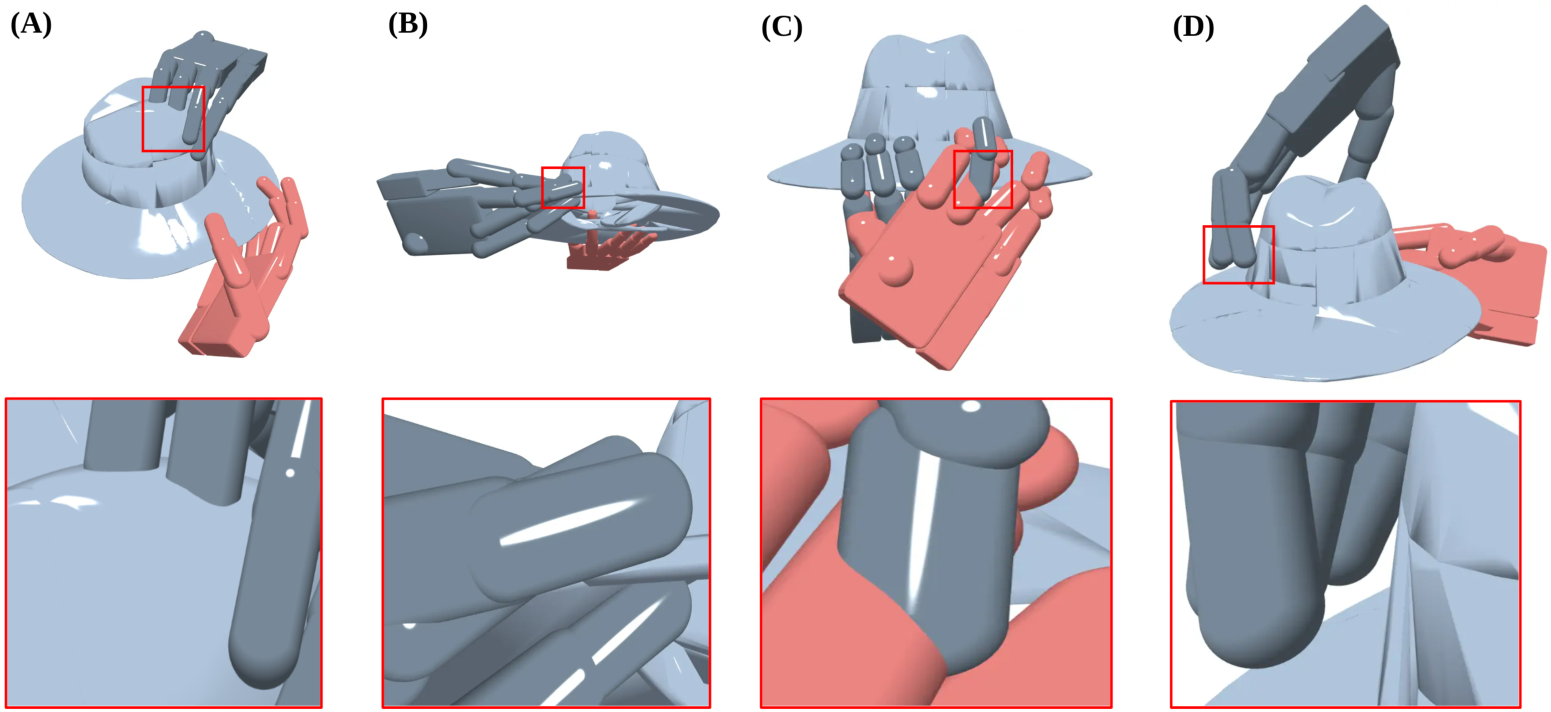
\includegraphics[width=0.86\columnwidth]{figs/selected/bimanual_grasp_penetration.png}
    \caption{Two failures of synthesised two-hand grasps, each enlarged at the
      contact: (A) a finger inside the object, (C) a finger inside the other hand.
      Both look plausible whole~\cite{bimangrasp_2024}.}
    \label{fig:bimanual-penetration}
    \licensed[panels (A) and (C) of Fig.~9]{Fig.~9 of Shao and Xiao, arXiv:2411.15903}{CC BY 4.0}{https://creativecommons.org/licenses/by/4.0/}
  \end{figure}}


\begin{document}

\title{Dexterous Manipulation, Single-Hand and Bimanual:\\
Machines, Simulators, and How Policies Are Trained}

\author{%
  \IEEEauthorblockN{Luai Abuelsamen}%
  \thanks{Corpus, notes and build at the repository accompanying this survey.
  Every claim in this paper traces to a structured note taken from a parsed source, and every
  count is recomputed from those notes at build time.}%
}

\markboth{Survey draft, \today}{Abuelsamen: Dexterous Manipulation, Single-Hand and Bimanual}
\maketitle

\begin{abstract}
%% Abstract. Converted from paper/ABSTRACT.md; prose unchanged.
%% Two facts are load-bearing here and not only in the body, because an abstract is quoted
%% alone: the penetration claim is scoped to this corpus and to a policy's own rollouts, in
%% the conclusion's words, and the clause that nobody was contacted before posting travels
%% with the accusation it qualifies. Keep this one paragraph and at most about 200 words.
A hand is dexterous when it can change an object's pose without putting the object down. This
survey divides that problem the way its sections do: the hands, the simulators they are trained
in, how policies are trained, two hands on one object, and how it is evaluated. It rests on 218
sources read into a structured row and their released code. Papers and their repositories state
different things: most method rows whose code could be read against the paper record a
disagreement, and nine are contradictions, each printed as a repository, a commit, a file and two
values; none of their authors was contacted before posting. No closed-loop policy in the corpus
reports interpenetration for the rollouts of its own trained policy, and few of the settled rows
handle it at all, though IsaacGymEnvs already computes that depth and gates a policy update on it.
Hardware has come apart from published work: most tabulated hands appear in no method row, and
several can be bought or built today. This survey re-runs no method and ranks nothing: on
penetration it supplies a measurement method and a count, not a threshold, and every coverage
statistic is a floor over what this extraction captured.

\end{abstract}

\begin{IEEEkeywords}
Dexterous manipulation, multi-fingered hands, bimanual manipulation, reinforcement learning,
imitation learning, physics simulation, contact modelling, benchmarking, reproducibility.
\end{IEEEkeywords}

\IEEEpeerreviewmaketitle

%% Section 1, Introduction. Converted from paper/sections/01_introduction.md.
\section{Introduction}
\label{sec:intro}

A hand is dexterous when it can change an object's pose without putting the object down. That
property, and not the finger count, is what separates a hand from a gripper. Bicchi
\cite{bicchi_grasping_chapter_2001} draws the same line in Sec.~1.1, between restraining an object
and ``manipulating objects with fingers, in contrast to manipulation with the robot arm''. Restraint
is a static question about whether the contacts prevent motion. In-hand manipulation is a dynamic
question about whether contacts can be broken and remade while the object stays held. An et al.
\cite{an_dexil_survey_2025} put the same idea in their abstract as the ability ``to skillfully
control, reorient, and manipulate objects through precise, coordinated finger movements and adaptive
force modulation''. Both definitions place the work in the fingers rather than in the arm.

The analytic theory answered the static question and stalled on the dynamic one. Form closure has
a first-order test on the grasp matrix and known contact counts, four in the plane and seven in
three dimensions for any polyhedron, per \cite{bicchi_grasping_chapter_2001} Sec.~1.3.1. Force closure
adds the wrench balance and the hand Jacobian. Neither delivers what a controller needs. The same
chapter states in Sec.~1.5 that ``force closure does not guarantee stability'', and its Sec.~1.8
names the reason the theory could not be pushed further, which is that ``the nonsmooth nature of
grasp dynamics, because of the unilateral constraints on displacements and forces, has made a
thorough analysis very difficult''. That verdict is one architect's, on one chapter, and this
survey did not survey the tradition it judges. Learned control did not solve those modelling
problems. It went around them by sampling a simulator instead of solving a model, and by scoring a
rollout instead of certifying a configuration. Of the 112 method papers in this corpus, 53 train
with reinforcement learning and 36 run in Isaac Gym, against 6 on its successor Isaac Lab.

Three things this survey measured are worth stating before the reader commits to 27,000 words. The
first is that papers disagree with their own released code. Sixty-two of the 112 method rows
released code that could be read against the paper, 38 of those record a discrepancy, and nine are
contradictions where the shipped code states a different objective from the published one. The
sharpest case is \cite{physhoi_2023}. Its \texttt{compute\_humanoid\_reward} hardcodes the object rotation and
rotation-velocity errors to zero, with the real computation commented out beside them, while the
reward table in its own paper lists weights of 0.1 and 0.01 for exactly those terms on GRAB. Its
position-only success criterion could not have caught that, and its headline 95.4 percent is cited
as a baseline. Section 5.8 classifies all 38, and seven further accusations an earlier draft made
were withdrawn under adversarial review and recorded beside the charge.
\figurename~\ref{fig:codegap} draws the narrowing.

% ---------------------------------------------------------------------------
% The first finding as a picture: the funnel from 112 method rows to the ten
% whose code contradicts the paper, with the 28 charges the survey withdrew
% drawn at the same weight as the 10 it kept. Written by
% tools/make_finding_figures.py from corpus/rows; the guard keeps the document
% compiling until it is there.
% ---------------------------------------------------------------------------
\makeatletter
\@ifundefined{fnLoaded}{\IfFileExists{figs/finding_numbers.tex}{% generated by tools/make_finding_figures.py; do not edit
% Every count the finding figures and their captions print, recomputed from corpus/rows.
\providecommand{\fnLoaded}{}
\providecommand{\fnRows}{112}
\providecommand{\fnCode}{62}
\providecommand{\fnDisagree}{38}
\providecommand{\fnKept}{9}
\providecommand{\fnOtherClass}{29}
\providecommand{\fnParse}{13}
\providecommand{\fnAbsent}{8}
\providecommand{\fnSkew}{4}
\providecommand{\fnInternal}{4}
\providecommand{\fnPenSettled}{96}
\providecommand{\fnPenHandled}{11}
\providecommand{\fnPenClosed}{4}
\providecommand{\fnPenOther}{7}
\providecommand{\fnPenRollout}{0}
\providecommand{\fnTrials}{39}
\providecommand{\fnTrialsMedian}{15}
\providecommand{\fnTrialsMode}{10}
\providecommand{\fnTrialsModeN}{16}
\providecommand{\fnTotals}{24}
\providecommand{\fnTotalsMin}{12}
\providecommand{\fnTotalsMax}{750}
\providecommand{\fnUnclear}{7}
}{}}{}
\makeatother
\begin{figure}[!t]
  \centering
  \IfFileExists{figs/fig_codegap.tex}{\resizebox{\columnwidth}{!}{% generated by tools/make_finding_figures.py; do not edit
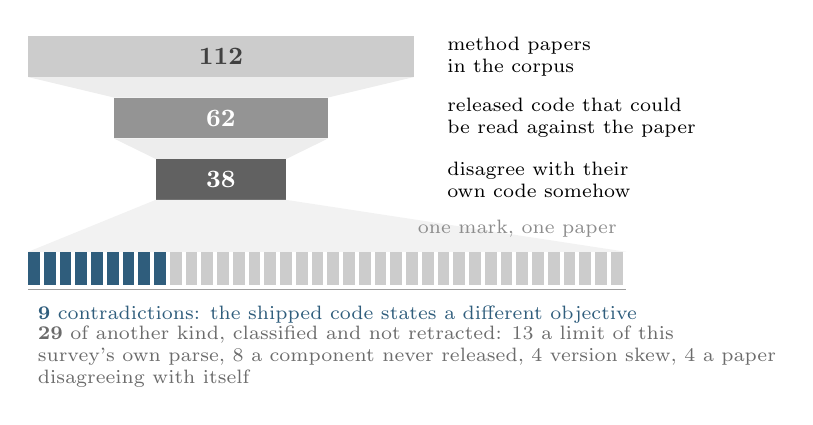
\begin{tikzpicture}[
  font=\footnotesize,
  bar/.style={draw=none,fill=black!62},
  barmid/.style={draw=none,fill=black!42},
  barlight/.style={draw=none,fill=black!20},
  baracc/.style={draw=none,fill=accent},
  seg/.style={draw=white,line width=0.5pt},
  lnk/.style={draw=black!38,line width=0.28pt},
  ghost/.style={draw=black!45,line width=0.3pt,dash pattern=on 1.2pt off 1.2pt},
  lbl/.style={font=\scriptsize},
  small/.style={font=\scriptsize\color{black!55}},
  num/.style={font=\scriptsize\color{black!55}},
]

\fill[barlight] (0.00,0.00) rectangle (4.90,-0.52);
\node[font=\small\bfseries\color{black!75}] at (2.45,-0.26) {112};
\node[lbl,anchor=west,align=left] at (5.20,-0.26) {method papers\\in the corpus};
\fill[black!7] (0.00,-0.52) -- (4.90,-0.52) -- (3.81,-0.78) -- (1.09,-0.78) -- cycle;
\fill[barmid] (1.09,-0.78) rectangle (3.81,-1.30);
\node[font=\small\bfseries\color{white}] at (2.45,-1.04) {62};
\node[lbl,anchor=west,align=left] at (5.20,-1.04) {released code that could\\be read against the paper};
\fill[black!7] (1.09,-1.30) -- (3.81,-1.30) -- (3.28,-1.56) -- (1.62,-1.56) -- cycle;
\fill[bar] (1.62,-1.56) rectangle (3.28,-2.08);
\node[font=\small\bfseries\color{white}] at (2.45,-1.82) {38};
\node[lbl,anchor=west,align=left] at (5.20,-1.82) {disagree with their\\own code somehow};
\fill[black!5] (1.62,-2.08) -- (3.28,-2.08) -- (7.60,-2.74) -- (0,-2.74) -- cycle;
\node[anchor=south east,font=\scriptsize\color{black!45}] at (7.60,-2.68) {one mark, one paper};
\fill[baracc] (0.00,-2.74) rectangle (0.15,-3.16);
\fill[baracc] (0.20,-2.74) rectangle (0.35,-3.16);
\fill[baracc] (0.40,-2.74) rectangle (0.55,-3.16);
\fill[baracc] (0.60,-2.74) rectangle (0.75,-3.16);
\fill[baracc] (0.80,-2.74) rectangle (0.95,-3.16);
\fill[baracc] (1.00,-2.74) rectangle (1.15,-3.16);
\fill[baracc] (1.20,-2.74) rectangle (1.35,-3.16);
\fill[baracc] (1.40,-2.74) rectangle (1.55,-3.16);
\fill[baracc] (1.60,-2.74) rectangle (1.75,-3.16);
\fill[barlight] (1.80,-2.74) rectangle (1.95,-3.16);
\fill[barlight] (2.00,-2.74) rectangle (2.15,-3.16);
\fill[barlight] (2.20,-2.74) rectangle (2.35,-3.16);
\fill[barlight] (2.40,-2.74) rectangle (2.55,-3.16);
\fill[barlight] (2.60,-2.74) rectangle (2.75,-3.16);
\fill[barlight] (2.80,-2.74) rectangle (2.95,-3.16);
\fill[barlight] (3.00,-2.74) rectangle (3.15,-3.16);
\fill[barlight] (3.20,-2.74) rectangle (3.35,-3.16);
\fill[barlight] (3.40,-2.74) rectangle (3.55,-3.16);
\fill[barlight] (3.60,-2.74) rectangle (3.75,-3.16);
\fill[barlight] (3.80,-2.74) rectangle (3.95,-3.16);
\fill[barlight] (4.00,-2.74) rectangle (4.15,-3.16);
\fill[barlight] (4.20,-2.74) rectangle (4.35,-3.16);
\fill[barlight] (4.40,-2.74) rectangle (4.55,-3.16);
\fill[barlight] (4.60,-2.74) rectangle (4.75,-3.16);
\fill[barlight] (4.80,-2.74) rectangle (4.95,-3.16);
\fill[barlight] (5.00,-2.74) rectangle (5.15,-3.16);
\fill[barlight] (5.20,-2.74) rectangle (5.35,-3.16);
\fill[barlight] (5.40,-2.74) rectangle (5.55,-3.16);
\fill[barlight] (5.60,-2.74) rectangle (5.75,-3.16);
\fill[barlight] (5.80,-2.74) rectangle (5.95,-3.16);
\fill[barlight] (6.00,-2.74) rectangle (6.15,-3.16);
\fill[barlight] (6.20,-2.74) rectangle (6.35,-3.16);
\fill[barlight] (6.40,-2.74) rectangle (6.55,-3.16);
\fill[barlight] (6.60,-2.74) rectangle (6.75,-3.16);
\fill[barlight] (6.80,-2.74) rectangle (6.95,-3.16);
\fill[barlight] (7.00,-2.74) rectangle (7.15,-3.16);
\fill[barlight] (7.20,-2.74) rectangle (7.35,-3.16);
\fill[barlight] (7.40,-2.74) rectangle (7.55,-3.16);
\draw[lnk] (0,-3.22) -- (7.60,-3.22);
\node[anchor=north west,align=left,font=\scriptsize\color{accent}] at (0,-3.30) {\textbf{9} contradictions: the shipped code states a different objective};
\node[anchor=north west,align=left,font=\scriptsize\color{black!58}] at (0,-3.56) {\textbf{29} of another kind, classified and not retracted: 13 a limit of this\\survey's own parse, 8 a component never released, 4 version skew, 4 a paper\\disagreeing with itself};
\end{tikzpicture}
}}{%
    \framebox[0.95\columnwidth]{\rule{0pt}{2.2cm}\textit{figs/fig\_codegap.tex pending}}}
  \caption{Papers disagree with their own released code, and most of the disagreements are this
  survey's own limits rather than theirs. Of the \fnRows{} method rows, \fnCode{} released code that
  could be read against the paper and \fnDisagree{} of those record a disagreement. The lower bar
  reopens those \fnDisagree{} at their own scale: \fnKept{} are contradictions, where the shipped
  code states a different objective from the published one, and \fnWithdrawn{} are withdrawn, most
  of them about this survey's own parse or about what a repository shipped rather than about the
  work. Further accusations
  an earlier draft made were withdrawn under adversarial review, each recorded in the accused row's
  \texttt{mismatch\_review} field beside the charge. Section~\ref{sec:train:code} classifies all
  \fnDisagree{} and names them.}
  \label{fig:codegap}
\end{figure}

The second is that the quantity most specific to a hand is the one closed-loop policies do not
record. Eleven of the 96 method rows whose notes settle the question address interpenetration at all,
seven of the eleven do it outside a closed-loop policy in a grasp synthesiser, a trajectory optimiser
or a contact model, and we found none that reports a penetration number for its own trained policy's
rollouts. The claim is about learned closed-loop control and not about the field. Grasp synthesis and
hand-object reconstruction have reported penetration depth and intersection volume as comparative
columns for years, and four rows of this corpus do it: OakInk \cite{oakink_2022} tabulates
penetration depth, solid intersection volume and simulation displacement across methods, BiDexGrasp
\cite{bidexgrasp_2026} prints penetration depth beside a prior method's, BimanGrasp
\cite{bimangrasp_2024} fails any grasp whose total penetration exceeds 1.5 mm, and TopoRetarget
\cite{toporetarget_2026} reports a maximum penetration and a share of frames past 2 mm against a
baseline retargeter. Every one of those numbers scores a pose or a reference trajectory rather than
the behaviour a trained policy produced, and it is the rollout that is missing. The
obstacle is not the engines. NVIDIA's own IsaacGymEnvs repository already computes a
per-environment maximum interpenetration depth in Warp and gates the policy update on a 1 mm
threshold. Section 7.3 has the file and the lines.

The third is that hardware and published work have come apart. 18 of the 33 hand rows in
Table~\ref{tab:hands-available} and Table~\ref{tab:hands-announced}
appear in no method row, and 7 of those can be bought today or built from
published designs. Thirty-five method rows run on the Allegro, whose weight, joint torque, payload
and price have no reachable source, because its product page returns HTTP 404 and everything
Table~\ref{tab:hands-available} confirms about it comes from its ROS driver.

None of those three findings is a first, and the audit behind the first of them is not a new idea.
Collberg and Proebsting \cite{collberg_repeatability_2016} examined 601 papers in computer systems
research for whether the code behind them could be obtained and built at all. Xu et al.
\cite{biocon_2026} align 48 bioinformatics projects with their publications at sentence-to-function
granularity under expert annotation, and SciCoQA \cite{scicoqa_2026} collects 92 real paper-code
discrepancies, mined from issue trackers and reproducibility reports, into a benchmark for detecting
such discrepancies automatically. In reinforcement learning the phenomenon itself is a known result.
Engstrom et al. \cite{engstrom_implementation_matters_2020} show that code-level optimisations
present only in the implementation account for most of PPO's reported gain over TRPO, and Meta-World+
\cite{metaworld_plus_2025} finds undocumented changes accumulated across one benchmark's own
versions, which make comparisons between those versions unfair. Both establish it on a single
codebase. The closest relative to the audit here is Knox et al. \cite{knox_reward_misdesign_2023},
who review nineteen reinforcement-learning publications on autonomous driving, characterise the
reward functions of ten of them exhaustively in a standard form, apply eight sanity checks and report
near-universal flaws in reward design. Their ground truth for what each reward was is the authors,
obtained through correspondence with them rather than by reading a released repository, and what they
establish is that published reward descriptions are incomplete: one of the ten described its reward,
discount factor, termination conditions and timestep thoroughly. Reading the code instead needs no
correspondence and supports a different charge, which is that where code exists it sometimes
contradicts the description. Raff \cite{raff_reproducibility_2019} took the opposite ground truth on
purpose, reimplementing 255 papers from their text alone and never opening the authors' code, which
is what makes the choice of arbiter a position rather than an accident.

So the claim here is narrow. We are aware of no prior work in robotics, and none in dexterous
manipulation, that reads a field's released reward implementations against the rewards its own papers
describe. Those seven comparisons are cited from outside this corpus and enter none of its counts.
The exposure of the claim belongs beside the count above: the evidence is a repository at a fetched
commit, each hash recorded in \texttt{corpus/code\_manifest.json}, and a repository at a commit is
evidence about that repository rather than about the run that produced a paper's numbers, because the
commit may postdate, precede or diverge from it. Hora \cite{hora_2022} states the problem in its own
README, which directs a reader to tag v0.0.1 and not to the commit parsed here to reproduce the
published numbers. The seven accusations an earlier draft withdrew are recorded in the accused rows
for the same reason: they are the evidence that the charges left standing were checked rather than
counted.

Fourteen corpus entries are themselves surveys or engine-comparison studies. Appendix D says what
each covers, on one set of columns tabulated in the repository. Four of the fourteen could
not be obtained, or were fetched too late to read, and are entered as such. Two of the three things
this survey adds are columns none of the fourteen fills. The first is
Table~\ref{tab:simulators}, which takes the engines \cite{nine_physics_engines_review_2024} scored
on documentation and usability and adds contact model, solver, iteration count, default timestep and
penetration exposure, conditioned on what a hand does to a solver. Erez et al.
\cite{physics_engine_comparison_2015} and Le Lidec et al. \cite{contact_models_comparison_2023} do
measure engines, on five engines and on four contact formulations, and neither surveys the field
those engines are used in. The second is two hands on one object as its own problem, which none of
the four field surveys gives more than a subsection.

The third is the penetration measurement, on an axis a predecessor had already named. Zhao et al.
\cite{zhao_dexhand_survey_2026} state in their Sec.~IV-C that the field assesses ``at least two
layers of performance: the quality of grasps or poses prior to execution, and the performance of
policies or generators during downstream execution'', and names ``physical plausibility, including
penetration'' as the most common criterion for the first layer. That is the reference-versus-rollout
split, named before this survey measured it, and the idea that contact quality belongs on the
evaluation axis is Zhao's. What Sec.~IV-C does not give is a measurement method or a count, and this
survey supplies those two. It does not supply a threshold. The 2 mm figure the field uses is taken
from \cite{toporetarget_2026} with no independent justification, the captured human grasps in
\cite{grab_2020} sit above it at 3.25 mm, and Section 7.7 states plainly that 2 mm is a simulator
convention rather than a physical bound.

The scope is single-hand and bimanual multi-fingered manipulation. Parallel-jaw manipulation
enters only as a comparison, which matters because 12 of the 112 method rows name a parallel-jaw
gripper among their own embodiments. Locomotion is excluded. Prosthetics are excluded except where
a hand crosses over into robot use, as the Psyonic Ability Hand does. The corpus holds 221
bibliography entries, of which 218 carry a structured row read from a note. Those 218 rows are 112
method papers, 33 hands, 15 simulators, 15 datasets, 14 benchmarks, 14 surveys, 8 tactile sensors
and 7 evaluation protocols. ``Method row'' throughout means one of the 112, and every headline count
in this survey has one of those eight classes as its denominator.

Two limits apply to every number here. This is a corpus of the learned era, which is a selection
effect and not a judgement: 138 of the 221 entries are dated 2024 or later, 16 predate 2018, and
two of the 112 method rows predate 2018, so any statement about a trend over time is a statement
about 2022 onward. The analytic tradition is represented by one readable chapter rather than
surveyed, and the planning line that took up the dynamic question directly, finger gaiting and
rolling-contact manipulation and regrasp planning, is not in the corpus at all. Every coverage
statistic is also a floor rather than a rate, because a value this survey failed to extract is
indistinguishable from a value the paper never reported, and every such miss converts a reporting
paper into a silent one.

\figurename~\ref{fig:field} puts the field on one page. Section 2 sets out the task families and what makes each
hard. Section 3 covers hands, their makers, and the gap between what is sold and what is run.
Section 4 covers simulators and contact models. Section 5 covers how policies are trained. Section
6 covers bimanual work as its own problem. Section 7 proposes an evaluation frame rather than a
leaderboard, and is the longest section. Section 8 states the gaps as claims with their evidence.
Section 9 says what to do about them, addressed to someone publishing, running experiments or
buying a hand. Appendix A is the method, and says where the tabulation this survey is built on
lives, which is the repository rather than these pages. Appendix B carries the three tables
Sections 3 and 4 read cells out of, Appendix C is the reward extraction, and Appendix D is the
comparison with the existing surveys.

% ---------------------------------------------------------------------------
% Figure 1, the field on one page. Full width: five columns of nodes with the
% routes that exist in the corpus. Drawn by tools/make_tikz_figures.py into
% figs/fig_field.tex; the guard keeps the document compiling until it is there.
% ---------------------------------------------------------------------------
\begin{figure*}[!t]
  \centering
  \IfFileExists{figs/fig_field.tex}{% generated by tools/make_tikz_figures.py; do not edit
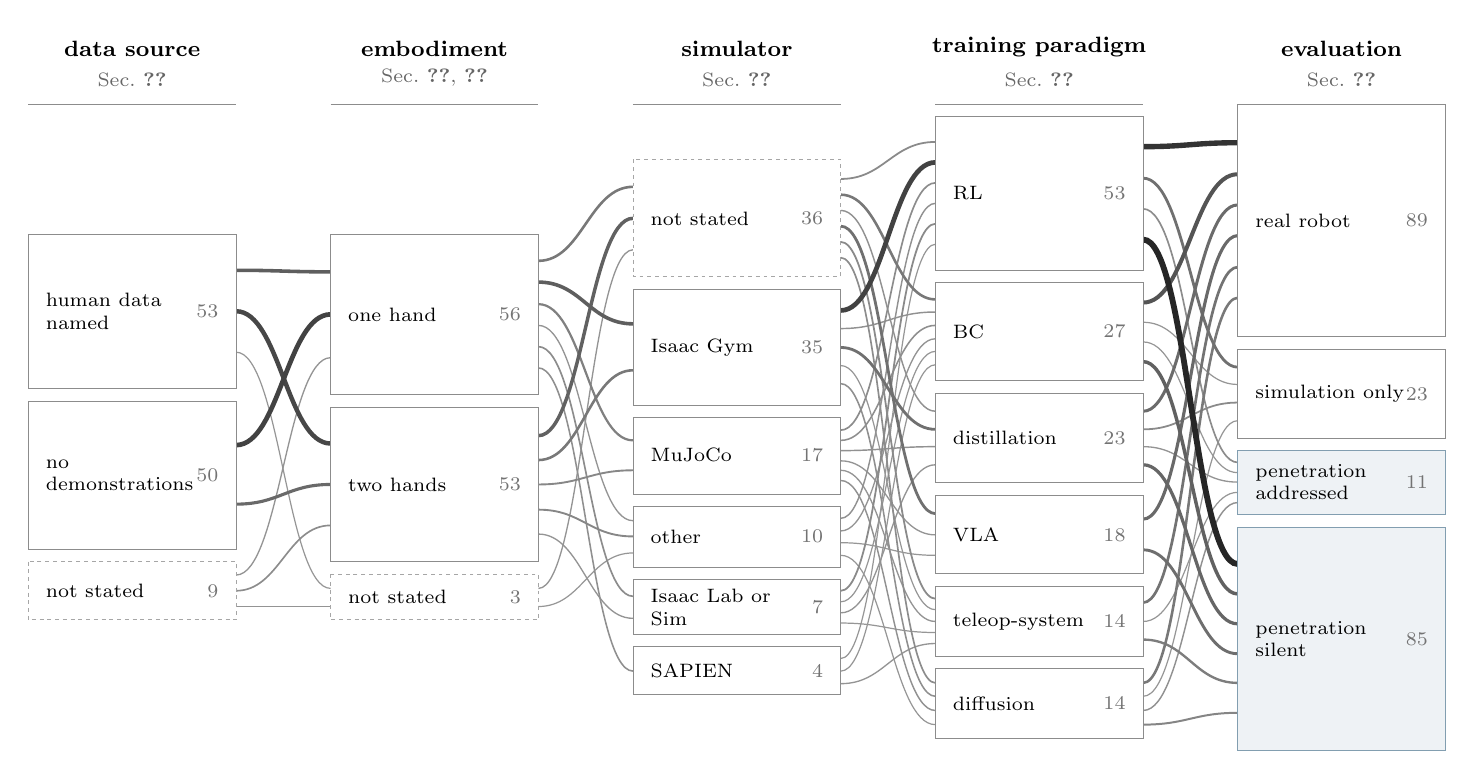
\begin{tikzpicture}[
  font=\scriptsize,
  bar/.style={draw=none,fill=black!62},
  barlight/.style={draw=none,fill=black!22},
  baracc/.style={draw=none,fill=accent},
  box/.style={draw=black!45,line width=0.3pt,inner sep=3pt,align=left},
  ghost/.style={draw=black!35,line width=0.3pt,dash pattern=on 1.4pt off 1.4pt,inner sep=3pt,align=left},
  lnk/.style={draw=black!38,line width=0.28pt},
  lbl/.style={font=\scriptsize},
  num/.style={font=\scriptsize\color{black!55}},
]

\draw[draw=black!41,line width=0.44pt] (2.64,-3.15) .. controls (3.19,-3.15) and (3.29,-6.15) .. (3.84,-6.15);
\draw[draw=black!41,line width=0.44pt] (6.48,-6.38) .. controls (7.03,-6.38) and (7.13,-5.70) .. (7.68,-5.70);
\draw[draw=black!41,line width=0.44pt] (10.32,-3.32) .. controls (10.87,-3.32) and (10.97,-6.42) .. (11.52,-6.42);
\draw[draw=black!41,line width=0.44pt] (10.32,-5.57) .. controls (10.87,-5.57) and (10.97,-5.73) .. (11.52,-5.73);
\draw[draw=black!41,line width=0.44pt] (10.32,-5.73) .. controls (10.87,-5.73) and (10.97,-7.88) .. (11.52,-7.88);
\draw[draw=black!41,line width=0.44pt] (10.32,-6.32) .. controls (10.87,-6.32) and (10.97,-3.14) .. (11.52,-3.14);
\draw[draw=black!41,line width=0.44pt] (10.32,-6.59) .. controls (10.87,-6.59) and (10.97,-6.71) .. (11.52,-6.71);
\draw[draw=black!41,line width=0.44pt] (10.32,-7.04) .. controls (10.87,-7.04) and (10.97,-1.78) .. (11.52,-1.78);
\draw[draw=black!41,line width=0.44pt] (10.32,-7.20) .. controls (10.87,-7.20) and (10.97,-3.31) .. (11.52,-3.31);
\draw[draw=black!41,line width=0.44pt] (14.16,-2.77) .. controls (14.71,-2.77) and (14.81,-3.56) .. (15.36,-3.56);
\draw[draw=black!41,line width=0.44pt] (14.16,-3.02) .. controls (14.71,-3.02) and (14.81,-4.68) .. (15.36,-4.68);
\draw[draw=black!41,line width=0.44pt] (14.16,-6.57) .. controls (14.71,-6.57) and (14.81,-4.93) .. (15.36,-4.93);
\draw[draw=black!41,line width=0.44pt] (14.16,-7.52) .. controls (14.71,-7.52) and (14.81,-4.02) .. (15.36,-4.02);
\draw[draw=black!42,line width=0.48pt] (2.64,-5.98) .. controls (3.19,-5.98) and (3.29,-3.22) .. (3.84,-3.22);
\draw[draw=black!42,line width=0.48pt] (2.64,-6.38) .. controls (3.19,-6.38) and (3.29,-6.38) .. (3.84,-6.38);
\draw[draw=black!42,line width=0.48pt] (6.48,-2.81) .. controls (7.03,-2.81) and (7.13,-5.29) .. (7.68,-5.29);
\draw[draw=black!42,line width=0.48pt] (6.48,-5.46) .. controls (7.03,-5.46) and (7.13,-6.53) .. (7.68,-6.53);
\draw[draw=black!42,line width=0.48pt] (6.48,-6.15) .. controls (7.03,-6.15) and (7.13,-1.85) .. (7.68,-1.85);
\draw[draw=black!42,line width=0.48pt] (10.32,-4.53) .. controls (10.87,-4.53) and (10.97,-5.47) .. (11.52,-5.47);
\draw[draw=black!42,line width=0.48pt] (10.32,-4.65) .. controls (10.87,-4.65) and (10.97,-6.57) .. (11.52,-6.57);
\draw[draw=black!42,line width=0.48pt] (10.32,-5.42) .. controls (10.87,-5.42) and (10.97,-2.98) .. (11.52,-2.98);
\draw[draw=black!42,line width=0.48pt] (10.32,-6.46) .. controls (10.87,-6.46) and (10.97,-4.58) .. (11.52,-4.58);
\draw[draw=black!42,line width=0.48pt] (10.32,-7.36) .. controls (10.87,-7.36) and (10.97,-6.85) .. (11.52,-6.85);
\draw[draw=black!42,line width=0.48pt] (14.16,-4.35) .. controls (14.71,-4.35) and (14.81,-4.80) .. (15.36,-4.80);
\draw[draw=black!43,line width=0.52pt] (10.32,-1.35) .. controls (10.87,-1.35) and (10.97,-3.90) .. (11.52,-3.90);
\draw[draw=black!43,line width=0.52pt] (10.32,-2.85) .. controls (10.87,-2.85) and (10.97,-2.64) .. (11.52,-2.64);
\draw[draw=black!43,line width=0.52pt] (10.32,-4.40) .. controls (10.87,-4.40) and (10.97,-4.35) .. (11.52,-4.35);
\draw[draw=black!43,line width=0.52pt] (10.32,-4.78) .. controls (10.87,-4.78) and (10.97,-7.70) .. (11.52,-7.70);
\draw[draw=black!43,line width=0.52pt] (10.32,-5.26) .. controls (10.87,-5.26) and (10.97,-1.26) .. (11.52,-1.26);
\draw[draw=black!43,line width=0.52pt] (14.16,-7.70) .. controls (14.71,-7.70) and (14.81,-5.06) .. (15.36,-5.06);
\draw[draw=black!44,line width=0.56pt] (6.48,-3.35) .. controls (7.03,-3.35) and (7.13,-7.20) .. (7.68,-7.20);
\draw[draw=black!44,line width=0.56pt] (10.32,-3.55) .. controls (10.87,-3.55) and (10.97,-7.52) .. (11.52,-7.52);
\draw[draw=black!44,line width=0.56pt] (10.32,-4.27) .. controls (10.87,-4.27) and (10.97,-2.81) .. (11.52,-2.81);
\draw[draw=black!45,line width=0.60pt] (2.64,-6.18) .. controls (3.19,-6.18) and (3.29,-5.35) .. (3.84,-5.35);
\draw[draw=black!45,line width=0.60pt] (6.48,-3.08) .. controls (7.03,-3.08) and (7.13,-6.25) .. (7.68,-6.25);
\draw[draw=black!45,line width=0.60pt] (10.32,-1.95) .. controls (10.87,-1.95) and (10.97,-7.35) .. (11.52,-7.35);
\draw[draw=black!45,line width=0.60pt] (10.32,-4.14) .. controls (10.87,-4.14) and (10.97,-1.00) .. (11.52,-1.00);
\draw[draw=black!45,line width=0.60pt] (14.16,-1.33) .. controls (14.71,-1.33) and (14.81,-4.55) .. (15.36,-4.55);
\draw[draw=black!46,line width=0.64pt] (10.32,-0.95) .. controls (10.87,-0.95) and (10.97,-0.48) .. (11.52,-0.48);
\draw[draw=black!46,line width=0.64pt] (10.32,-1.75) .. controls (10.87,-1.75) and (10.97,-6.28) .. (11.52,-6.28);
\draw[draw=black!46,line width=0.64pt] (10.32,-6.18) .. controls (10.87,-6.18) and (10.97,-1.52) .. (11.52,-1.52);
\draw[draw=black!46,line width=0.64pt] (14.16,-4.13) .. controls (14.71,-4.13) and (14.81,-3.79) .. (15.36,-3.79);
\draw[draw=black!47,line width=0.68pt] (6.48,-4.83) .. controls (7.03,-4.83) and (7.13,-4.65) .. (7.68,-4.65);
\draw[draw=black!47,line width=0.68pt] (6.48,-5.15) .. controls (7.03,-5.15) and (7.13,-5.49) .. (7.68,-5.49);
\draw[draw=black!48,line width=0.72pt] (14.16,-7.88) .. controls (14.71,-7.88) and (14.81,-7.73) .. (15.36,-7.73);
\draw[draw=black!50,line width=0.80pt] (6.48,-2.54) .. controls (7.03,-2.54) and (7.13,-4.27) .. (7.68,-4.27);
\draw[draw=black!51,line width=0.85pt] (14.16,-6.80) .. controls (14.71,-6.80) and (14.81,-7.35) .. (15.36,-7.35);
\draw[draw=black!53,line width=0.93pt] (6.48,-1.99) .. controls (7.03,-1.99) and (7.13,-1.05) .. (7.68,-1.05);
\draw[draw=black!53,line width=0.93pt] (6.48,-4.52) .. controls (7.03,-4.52) and (7.13,-3.38) .. (7.68,-3.38);
\draw[draw=black!53,line width=0.93pt] (10.32,-1.15) .. controls (10.87,-1.15) and (10.97,-2.48) .. (11.52,-2.48);
\draw[draw=black!53,line width=0.93pt] (14.16,-7.35) .. controls (14.71,-7.35) and (14.81,-2.46) .. (15.36,-2.46);
\draw[draw=black!55,line width=0.97pt] (14.16,-6.33) .. controls (14.71,-6.33) and (14.81,-2.07) .. (15.36,-2.07);
\draw[draw=black!56,line width=1.01pt] (10.32,-1.55) .. controls (10.87,-1.55) and (10.97,-5.20) .. (11.52,-5.20);
\draw[draw=black!56,line width=1.01pt] (10.32,-3.09) .. controls (10.87,-3.09) and (10.97,-4.13) .. (11.52,-4.13);
\draw[draw=black!56,line width=1.01pt] (14.16,-0.94) .. controls (14.71,-0.94) and (14.81,-3.34) .. (15.36,-3.34);
\draw[draw=black!57,line width=1.05pt] (14.16,-5.66) .. controls (14.71,-5.66) and (14.81,-6.98) .. (15.36,-6.98);
\draw[draw=black!58,line width=1.09pt] (14.16,-3.90) .. controls (14.71,-3.90) and (14.81,-1.28) .. (15.36,-1.28);
\draw[draw=black!59,line width=1.13pt] (2.64,-5.08) .. controls (3.19,-5.08) and (3.29,-4.83) .. (3.84,-4.83);
\draw[draw=black!59,line width=1.13pt] (14.16,-5.27) .. controls (14.71,-5.27) and (14.81,-1.67) .. (15.36,-1.67);
\draw[draw=black!60,line width=1.17pt] (14.16,-4.58) .. controls (14.71,-4.58) and (14.81,-6.60) .. (15.36,-6.60);
\draw[draw=black!62,line width=1.25pt] (6.48,-4.21) .. controls (7.03,-4.21) and (7.13,-1.45) .. (7.68,-1.45);
\draw[draw=black!62,line width=1.25pt] (14.16,-3.27) .. controls (14.71,-3.27) and (14.81,-6.22) .. (15.36,-6.22);
\draw[draw=black!63,line width=1.29pt] (2.64,-2.11) .. controls (3.19,-2.11) and (3.29,-2.13) .. (3.84,-2.13);
\draw[draw=black!63,line width=1.29pt] (6.48,-2.26) .. controls (7.03,-2.26) and (7.13,-2.79) .. (7.68,-2.79);
\draw[draw=black!67,line width=1.45pt] (14.16,-2.52) .. controls (14.71,-2.52) and (14.81,-0.89) .. (15.36,-0.89);
\draw[draw=black!72,line width=1.61pt] (2.64,-2.63) .. controls (3.19,-2.63) and (3.29,-4.31) .. (3.84,-4.31);
\draw[draw=black!74,line width=1.70pt] (2.64,-4.33) .. controls (3.19,-4.33) and (3.29,-2.67) .. (3.84,-2.67);
\draw[draw=black!74,line width=1.70pt] (10.32,-2.62) .. controls (10.87,-2.62) and (10.97,-0.74) .. (11.52,-0.74);
\draw[draw=black!80,line width=1.94pt] (14.16,-0.54) .. controls (14.71,-0.54) and (14.81,-0.49) .. (15.36,-0.49);
\draw[draw=black!85,line width=2.10pt] (14.16,-1.72) .. controls (14.71,-1.72) and (14.81,-5.84) .. (15.36,-5.84);
\node[font=\footnotesize\bfseries,anchor=south] at (1.32,0.48) {data source};
\node[font=\scriptsize\color{black!60},anchor=south] at (1.32,0.10) {Sec.~\ref{sec:train:human}};
\draw[draw=black!45,line width=0.4pt] (0.00,0.00) -- (2.64,0.00);
\draw[box,fill=white] (0.00,-1.65) rectangle (2.64,-3.61);
\node[lbl,anchor=west,align=left] at (0.10,-2.63) {human data\\named};
\node[num,anchor=east] at (2.54,-2.63) {53};
\draw[box,fill=white] (0.00,-3.77) rectangle (2.64,-5.65);
\node[lbl,anchor=west,align=left] at (0.10,-4.71) {no\\demonstrations};
\node[num,anchor=east] at (2.54,-4.71) {50};
\draw[ghost,fill=white] (0.00,-5.81) rectangle (2.64,-6.55);
\node[lbl,anchor=west,align=left] at (0.10,-6.18) {not stated};
\node[num,anchor=east] at (2.54,-6.18) {9};
\node[font=\footnotesize\bfseries,anchor=south] at (5.16,0.48) {embodiment};
\node[font=\scriptsize\color{black!60},anchor=south] at (5.16,0.10) {Sec.~\ref{sec:hands},~\ref{sec:bimanual}};
\draw[draw=black!45,line width=0.4pt] (3.84,0.00) -- (6.48,0.00);
\draw[box,fill=white] (3.84,-1.65) rectangle (6.48,-3.69);
\node[lbl,anchor=west,align=left] at (3.94,-2.67) {one hand};
\node[num,anchor=east] at (6.38,-2.67) {56};
\draw[box,fill=white] (3.84,-3.85) rectangle (6.48,-5.81);
\node[lbl,anchor=west,align=left] at (3.94,-4.83) {two hands};
\node[num,anchor=east] at (6.38,-4.83) {53};
\draw[ghost,fill=white] (3.84,-5.97) rectangle (6.48,-6.55);
\node[lbl,anchor=west,align=left] at (3.94,-6.26) {not stated};
\node[num,anchor=east] at (6.38,-6.26) {3};
\node[font=\footnotesize\bfseries,anchor=south] at (9.00,0.48) {simulator};
\node[font=\scriptsize\color{black!60},anchor=south] at (9.00,0.10) {Sec.~\ref{sec:simulators}};
\draw[draw=black!45,line width=0.4pt] (7.68,0.00) -- (10.32,0.00);
\draw[ghost,fill=white] (7.68,-0.70) rectangle (10.32,-2.19);
\node[lbl,anchor=west,align=left] at (7.78,-1.45) {not stated};
\node[num,anchor=east] at (10.22,-1.45) {36};
\draw[box,fill=white] (7.68,-2.35) rectangle (10.32,-3.82);
\node[lbl,anchor=west,align=left] at (7.78,-3.09) {Isaac Gym};
\node[num,anchor=east] at (10.22,-3.09) {35};
\draw[box,fill=white] (7.68,-3.98) rectangle (10.32,-4.95);
\node[lbl,anchor=west,align=left] at (7.78,-4.46) {MuJoCo};
\node[num,anchor=east] at (10.22,-4.46) {17};
\draw[box,fill=white] (7.68,-5.11) rectangle (10.32,-5.88);
\node[lbl,anchor=west,align=left] at (7.78,-5.49) {other};
\node[num,anchor=east] at (10.22,-5.49) {10};
\draw[box,fill=white] (7.68,-6.04) rectangle (10.32,-6.73);
\node[lbl,anchor=west,align=left] at (7.78,-6.39) {Isaac Lab or\\Sim};
\node[num,anchor=east] at (10.22,-6.39) {7};
\draw[box,fill=white] (7.68,-6.89) rectangle (10.32,-7.50);
\node[lbl,anchor=west,align=left] at (7.78,-7.20) {SAPIEN};
\node[num,anchor=east] at (10.22,-7.20) {4};
\node[font=\footnotesize\bfseries,anchor=south] at (12.84,0.48) {training paradigm};
\node[font=\scriptsize\color{black!60},anchor=south] at (12.84,0.10) {Sec.~\ref{sec:training}};
\draw[draw=black!45,line width=0.4pt] (11.52,0.00) -- (14.16,0.00);
\draw[box,fill=white] (11.52,-0.15) rectangle (14.16,-2.11);
\node[lbl,anchor=west,align=left] at (11.62,-1.13) {RL};
\node[num,anchor=east] at (14.06,-1.13) {53};
\draw[box,fill=white] (11.52,-2.27) rectangle (14.16,-3.51);
\node[lbl,anchor=west,align=left] at (11.62,-2.89) {BC};
\node[num,anchor=east] at (14.06,-2.89) {27};
\draw[box,fill=white] (11.52,-3.67) rectangle (14.16,-4.81);
\node[lbl,anchor=west,align=left] at (11.62,-4.24) {distillation};
\node[num,anchor=east] at (14.06,-4.24) {23};
\draw[box,fill=white] (11.52,-4.97) rectangle (14.16,-5.96);
\node[lbl,anchor=west,align=left] at (11.62,-5.47) {VLA};
\node[num,anchor=east] at (14.06,-5.47) {18};
\draw[box,fill=white] (11.52,-6.12) rectangle (14.16,-7.01);
\node[lbl,anchor=west,align=left] at (11.62,-6.57) {teleop-system};
\node[num,anchor=east] at (14.06,-6.57) {14};
\draw[box,fill=white] (11.52,-7.17) rectangle (14.16,-8.05);
\node[lbl,anchor=west,align=left] at (11.62,-7.61) {diffusion};
\node[num,anchor=east] at (14.06,-7.61) {14};
\node[font=\footnotesize\bfseries,anchor=south] at (16.68,0.48) {evaluation};
\node[font=\scriptsize\color{black!60},anchor=south] at (16.68,0.10) {Sec.~\ref{sec:evaluation}};
\draw[draw=black!45,line width=0.4pt] (15.36,0.00) -- (18.00,0.00);
\draw[box,fill=white] (15.36,-0.00) rectangle (18.00,-2.95);
\node[lbl,anchor=west,align=left] at (15.46,-1.48) {real robot};
\node[num,anchor=east] at (17.90,-1.48) {89};
\draw[box,fill=white] (15.36,-3.11) rectangle (18.00,-4.24);
\node[lbl,anchor=west,align=left] at (15.46,-3.68) {simulation only};
\node[num,anchor=east] at (17.90,-3.68) {23};
\draw[box,fill=accent!8,draw=accent!60] (15.36,-4.40) rectangle (18.00,-5.21);
\node[lbl,anchor=west,align=left] at (15.46,-4.80) {penetration\\addressed};
\node[num,anchor=east] at (17.90,-4.80) {11};
\draw[box,fill=accent!8,draw=accent!60] (15.36,-5.37) rectangle (18.00,-8.21);
\node[lbl,anchor=west,align=left] at (15.46,-6.79) {penetration\\silent};
\node[num,anchor=east] at (17.90,-6.79) {85};
\end{tikzpicture}
}{%
    \framebox[0.7\textwidth]{\rule{0pt}{2.2cm}\textit{figs/fig\_field.tex pending}}}
  \caption{The field on one page. Data sources, embodiment, simulator, training paradigm and
  evaluation, with nodes sized by how many corpus papers sit in them and edges drawn only for
  routes the corpus actually contains. The routes converge: almost everything ends in a policy
  trained in a GPU simulator and distilled to vision.}
  \label{fig:field}
\end{figure*}

%% Section 2, A taxonomy of the problem. Converted from paper/sections/02_taxonomy.md.
\section{A taxonomy of the problem}
\label{sec:taxonomy}

\subsection{Task families}
\label{sec:taxonomy:tasks}

The six families below are read off the rows rather than imposed on them, and Sec.~2.1's closing
paragraph says what they miss. Grasping is the largest. Fifty-seven of the 112 method rows carry the
grasp label, the labels are not exclusive, and one paper can sit in several families. Success is a
lift that survives a hold, and the thresholds differ by more than an order of magnitude. DexGraspVLA
\cite{dexgraspvla_2025} requires the object ``held 10 cm above the table for 20 s'', while Omnigrasp
\cite{omnigrasp_2024} requires it ``held at least 0.5 s in simulation''. What makes grasping hard at
scale is the continuum of starting configurations. UniDexGrasp++ \cite{unidexgrasp_pp_2023} states
it in Sec.~4.3, that ``we are dealing with an infinite number of tasks considering the initial
object pose can change continuously''.

Functional and tool use is second with 45 rows. It is the family where a stable grasp can still be
the wrong answer. Dexterous Functional Grasping \cite{dexterous_functional_grasping_2023} gives the
case in Sec.~2.1, that ``grabbing a
hammer from the head or handle are both equally valid ways of using it'', and only one of the two
lets the tool be used. Success is defined against the tool's function, and the field has no shared
way to state it.

In-hand reorientation has 31 rows and the most settled criteria, because the community inherited one
number. OpenAI \cite{openai_dexterity_2018} declared the goal achieved below 0.4 rad of orientation
error, DeXtreme \cite{dextreme_2022} keeps 0.4 rad at test time against a 0.1 rad training
tolerance, and Eureka \cite{eureka_2023}
counts consecutive successes at 0.1 rad. A shared tolerance is not a shared protocol, because the
stopping rule differs. Visual Dexterity \cite{visual_dexterity_2022} measures error ``when the
controller predicts it has
reached the goal and stops'', which makes the policy a judge of its own trial.

Tracking a human reference has 12 rows and inverts the problem. The target is a trajectory rather
than an endpoint, so success is a per-frame error band. ManipTrans \cite{maniptrans_2025} requires
all four of 30
degrees of rotation, 3 cm of translation, 8 cm of joint error and 6 cm of fingertip error. The
difficulty is that the reference came from a human hand and was never dynamically feasible for the
robot. DexMachina \cite{dexmachina_2025} warns in App.~B.4 that scoring by timesteps inside the
thresholds makes
``the results highly sensitive to the threshold values''.

Bimanual coordination has 43 rows and handover has 10. Handover is the smallest family and the one
whose failure has a single moment, because the giver must release only after the receiver has the
object. Dynamic Handover \cite{dynamic_handover_2023} reports a hit rate above its success rate and
blames the gap in Sec.~5.4 on ``occasional challenges encountered during the grasping phase of the
catcher''. Not every paper here learns both sides. In \cite{dexterous_handover_2025} only the
receiver is learned and the giver is a scripted arm.

Those six families do not cover the corpus. Twenty-four of the 112 method rows carry a label from
outside them and eight carry no label from the six at all. Twenty are labelled \texttt{other},
mostly generalist policies evaluated on a task suite rather than on a dexterous task family, among
them \cite{pi0_2024,pi05_2025,pistar06_2025,openvla_2024} and \cite{gemini_robotics_15_2025}. Three
adjacent families are named here rather than absorbed. Locomanipulation is
\cite{humanplus_2024,omnih2o_2024} and \cite{groot_n16_2025}, where the base is not fixed and the
gravity argument below changes character. Piano playing is \cite{robopianist_2023,rp1m_2024} and
\cite{pianomime_2024}, discussed in Section 6, where success is a per-timestep F1 against a MIDI
score rather than an object pose. Deformable manipulation is \cite{dexdeform_2023}, whose object
carries its own state and its own physics. Ferrari and Canny's grasp-quality measure
\cite{ferrari_canny_1992} carries no task label, because it is a measure rather than a task.
Table~\ref{tab:tasks}'s six rows are the families with enough papers to compare, and not a partition
of the corpus.

\subsection{What makes dexterous control hard}
\label{sec:taxonomy:hard}

Contact is non-smooth, and that is a property of the problem rather than of any solver. Bicchi
\cite{bicchi_grasping_chapter_2001} states in Sec.~1.2 that contact constraints are unilateral, and
that losing a contact ``involves an abrupt change of the structure of the model under
consideration''. Its Sec.~1.4 gives the sharper version, that a rod sliding on rough ground has
configurations with no consistent solution and configurations with more than one. Simulators inherit
the difficulty. The re-implementation study \cite{contact_models_comparison_2023} concludes in
Sec.~V that ``there is no fully satisfactory approach at the moment, as all existing solutions
compromise either accuracy, robustness, or efficiency''. Pang et al.
\cite{pang_global_planning_2022} treat non-smoothness as the thing to remove, curating every contact
pair in Sec.~III-D so that contact points and normals change smoothly.

The hand has more actuators than the object has degrees of freedom and is still short of authority
over it. The object moves only through contacts, and the contacts are what cannot be commanded.
Bicchi \cite{bicchi_grasping_chapter_2001} states in Sec.~1.4 that in multifingered grasps ``the
number of independent contact forces is much larger than the number of actuators. Thus, from a
controllability standpoint, not all the contact forces are controllable''.

Vision is occluded by the hand doing the work. Bai et al. \cite{bai_unified_manip_survey_2025} name
it in Sec.~4.3,
that ``occlusion hampers object tracking''. DexPoint \cite{dexpoint_2022} keeps vision and adds
imagined hand points
to the point cloud. Yin et al. \cite{rotating_without_seeing_2023} remove vision entirely and rotate
objects from
16 binary touch sensors over the palm, links and fingertips.

Gravity direction changes the task rather than scaling it. Visual Dexterity
\cite{visual_dexterity_2022} states that reorientation with the hand below the object ``is much
easier'', because ``with a downward-facing hand, the hand must manipulate the object while
simultaneously counteracting gravity''. AnyRotate \cite{anyrotate_2024} makes the direction a
randomised variable by ``randomly initializing hand orientations between episodes'', and its
Sec.~5.3 measures the cost, with performance dropping progressively from palm up and palm down,
through base up and base down, to thumb up and thumb down.

\subsection{Single hand versus two}
\label{sec:taxonomy:twohands}

Three counts describe two hands and they measure different things. Fifty-three of the 112 method
rows record two hands on the robot, which is the \texttt{bimanual} field. Forty-three carry the
\texttt{bimanual-coord} task label, the narrower claim that coordinating the hands is the task. Section 6
narrows again, to the 28 rows whose notes place a learned closed-loop controller on two
multi-fingered hands, and its opening paragraph names every exclusion that takes the 53 down to
the 28. That 28 is the denominator for every architecture count in this survey. Every bimanual
claim here names which of the three it uses.

Four things genuinely change when the second hand arrives. Contact stays non-smooth, occlusion
stays, and gravity stays the same problem.

Role asymmetry is the first. AsymDex \cite{asymdex_2024} assigns a dominant hand with full finger
and wrist control and a facilitating hand with 6-DoF base pose only, so that ``the facilitating hand
repositions and reorients one object, while the dominant hand performs complex manipulations''.

The second is that two hands on one object close a kinematic chain through the object. In
\cite{bicchi_grasping_chapter_2001} Sec.~1.4 the hand and object dynamics are separate and are
``linked through the n rigid-body contact constraints''. A second hand adds a second constraint set
on the same object rather than a second independent problem. That is where physical plausibility
fails first. BimanGrasp \cite{bimangrasp_2024} is the corpus row that measures it, rejecting a
synthesised grasp when ``total penetrations exceeded 1.5 mm'' and reporting in Sec.~IV-C that
``penetration remains the primary cause of grasp failure''.

The third is two-arm collision, which does not exist for one hand. DyDexHandover
\cite{dydexhandover_2025} resets an episode when ``any unintended arm contact with the environment
or self-collisions'' occurs. Bunny-VisionPro \cite{bunny_visionpro_2024} pays for it in the
controller, where adding a sphere-approximated self-collision cost raises motion-control time from
0.74 ms to 7.85 ms. Bidex \cite{bidex_teleop_2024} solves it in hardware, mounting the hands so the
human arm and the teacher arm ``are perpendicular to each other and do not collide''. DexMimicGen
\cite{dexmimicgen_2024} states plainly that it does not handle inter-arm collision at all.

The fourth is the doubled action space. Bi-DexHands \cite{bidexhands_2022} runs 20 tasks on two
Shadow Hands and finds single-agent PPO beating multi-agent RL on most of them, offering in Sec.~5.2
that ``PPO algorithm is able to use all observations for training the policy, while MARL can only
use partial observations''. AsymDex \cite{asymdex_2024} attacks the dimensionality from the other
side, halving the observation and action dimension through its role split and a frame relative to
the facilitating hand's object.

% ---------------------------------------------------------------------------
% Table 1 is hand-written rather than generated from corpus/rows, so it is
% carried in this section file instead of tex/tables/. Full text width.
% ---------------------------------------------------------------------------
\begin{table*}[!t]
  \caption{Task families against the properties that define success.}
  \label{tab:tasks}
  \centering\scriptsize
  \begin{tabular}{@{}L{0.085\textwidth}L{0.150\textwidth}L{0.150\textwidth}L{0.145\textwidth}L{0.130\textwidth}L{0.240\textwidth}@{}}
    \toprule
    \rowcolor{wash} \hdr{task family} & \hdr{what is held} & \hdr{what moves} & \hdr{what gravity does} & \hdr{what counts as failure} & \hdr{shortest honest success criterion} \\
    \midrule
    In-hand reorientation &
    one rigid object, held by the fingers for the whole episode &
    the object's orientation in the palm frame, while contacts break and remake &
    a disturbance whose direction is set by hand orientation, and a load to counteract with the palm down, \cite{visual_dexterity_2022} &
    the object leaves the hand, e.g.\ the fall reset at goal distance 0.24 m in \cite{dextreme_2022} &
    orientation error below a stated tolerance under a stated stopping rule, 0.4 rad in \cite{openai_dexterity_2018} and \cite{dextreme_2022}, 0.1 rad in \cite{eureka_2023} \\
    \addlinespace[2.5pt]
    Grasping &
    nothing at the start, the object rests on a support &
    the hand closes, then the object is lifted clear &
    the test itself, since the grasp exists to resist it &
    no lift, or a drop inside the hold window &
    a stated lift height held for a stated duration, 10 cm for 20 s in \cite{dexgraspvla_2025}, 10 cm to episode end in \cite{graspxl_2024}, 0.5 s in \cite{omnigrasp_2024} \\
    \addlinespace[2.5pt]
    Functional and tool use &
    a tool, held in the pose its function requires rather than the most stable one &
    the tool's own joint, or the tool acting on a second object &
    secondary, the function dominates &
    a stable grasp in the wrong place, \cite{dexterous_functional_grasping_2023} &
    no agreed criterion. Criteria range from never dropping the object, \cite{dexterous_functional_grasping_2023}, to a four-point rubric, \cite{dexvla_2025}. The one mechanical threshold is holding the tool joint past a commanded angle for the episode, \cite{articulated_tools_inhand_2025} \\
    \addlinespace[2.5pt]
    Tracking a human reference &
    whatever the human held in the captured clip &
    hand and object follow a recorded trajectory under physics &
    full, and the reference never obeyed it, so the reference is not dynamically feasible &
    per-frame error leaves the band, or the object drops &
    all stated per-frame errors below threshold for the whole clip, 30 deg and 3 cm and 8 cm joint and 6 cm fingertip in \cite{maniptrans_2025}. Thresholds are not comparable across papers, and DexMachina \cite{dexmachina_2025} calls the results ``highly sensitive to the threshold values'' \\
    \addlinespace[2.5pt]
    Bimanual coordination &
    one object by two hands, or one object per hand &
    both hands, the object, and the relative pose of the hands &
    can be carried by one hand while the other acts, \cite{asymdex_2024} &
    the object drops, the arms collide, or the hands work against each other &
    no agreed criterion. Task-specific thresholds dominate, e.g.\ 0.035 m block-to-cup distance in \cite{asymdex_2024}. The one criterion with a physical-plausibility gate is 2.0 s of hold with total penetration under 1.5 mm, \cite{bimangrasp_2024} \\
    \addlinespace[2.5pt]
    Handover and in-hand transfer &
    by the giver at the start, by the receiver at the end &
    the object crosses between hands, released only after it is regained &
    unopposed during the exchange, and total in a thrown transfer, \cite{dynamic_handover_2023} &
    a drop at the moment of release, and the catcher's grasp phase, \cite{dynamic_handover_2023} Sec.~5.4 &
    the receiver holds the object and moves it clear, more than 10 cm from the first hand in \cite{hato_visuotactile_2024}, or holds it to episode end in \cite{dydexhandover_2025} \\
    \bottomrule
  \end{tabular}
\end{table*}

Two cells say the field has no agreed criterion, and both are in families where a second body is
involved. A criterion naming a distance, a duration and a trial count can be re-run by someone else.
A rubric cannot, and Section 7 takes up what follows from that.

%% Section 3, Hands and who makes them. Converted from paper/sections/03_hands.md.
\section{Hands and who makes them}
\label{sec:hands}

\subsection{The design axes}
\label{sec:hands:axes}

% --- reproduced plates ------------------------------------------------------
% tex/figs/plates.tex defines one command per selected photograph. Load it here
% if nothing has loaded it already, so this section carries its own plates
% whether or not the preamble inputs the file. The \providecommand before each
% call makes a missing plate an empty command rather than an error. Every plate
% carries \pending: read tex/PERMISSIONS.md before this goes anywhere.
% ---------------------------------------------------------------------------
\makeatletter
\@ifundefined{plateLeapOverview}{\IfFileExists{figs/plates.tex}{% The one reproduced plate.
% Rebuilt from its source PDF by tools/relayout_plates.py; see tex/figs/SELECTED.md for the crop
% box and tex/PERMISSIONS.md for the licence it is used under.
%
% A plate is kept only where a photograph or a render carries something a drawing cannot, and
% only where the paper has the right to print it without asking anyone. Everything else that was
% reproduced has been redrawn in the paper's own style (figs/fig_transmission, fig_collision,
% fig_tactiledepth, fig_contactlabel, fig_retarget) or dropped, because the prose already made the
% point or because no honest drawing could be made from what the corpus records. That took
% eighteen plates to one, eleven visual styles to four, and eleven open permissions to none.
%
% The survivor is single column and single panel. It is not a `figure*`: a borrowed plate has not
% earned the page width.
%
% One command for it. A section author places it by writing
%   \plateGraspPenetration
% at the point in the section where the float should be anchored, once: a plate called twice
% prints twice, on two pages, under two numbers.
%
% The plate credits its source inside its own caption with \src or \cite, and carries \licensed as
% well, because its source is CC BY 4.0 and the licence asks for an attribution line.

% ========================================================== Sec. VI, two hands

\newcommand{\plateGraspPenetration}{%
  \begin{figure}[t]
    \centering
    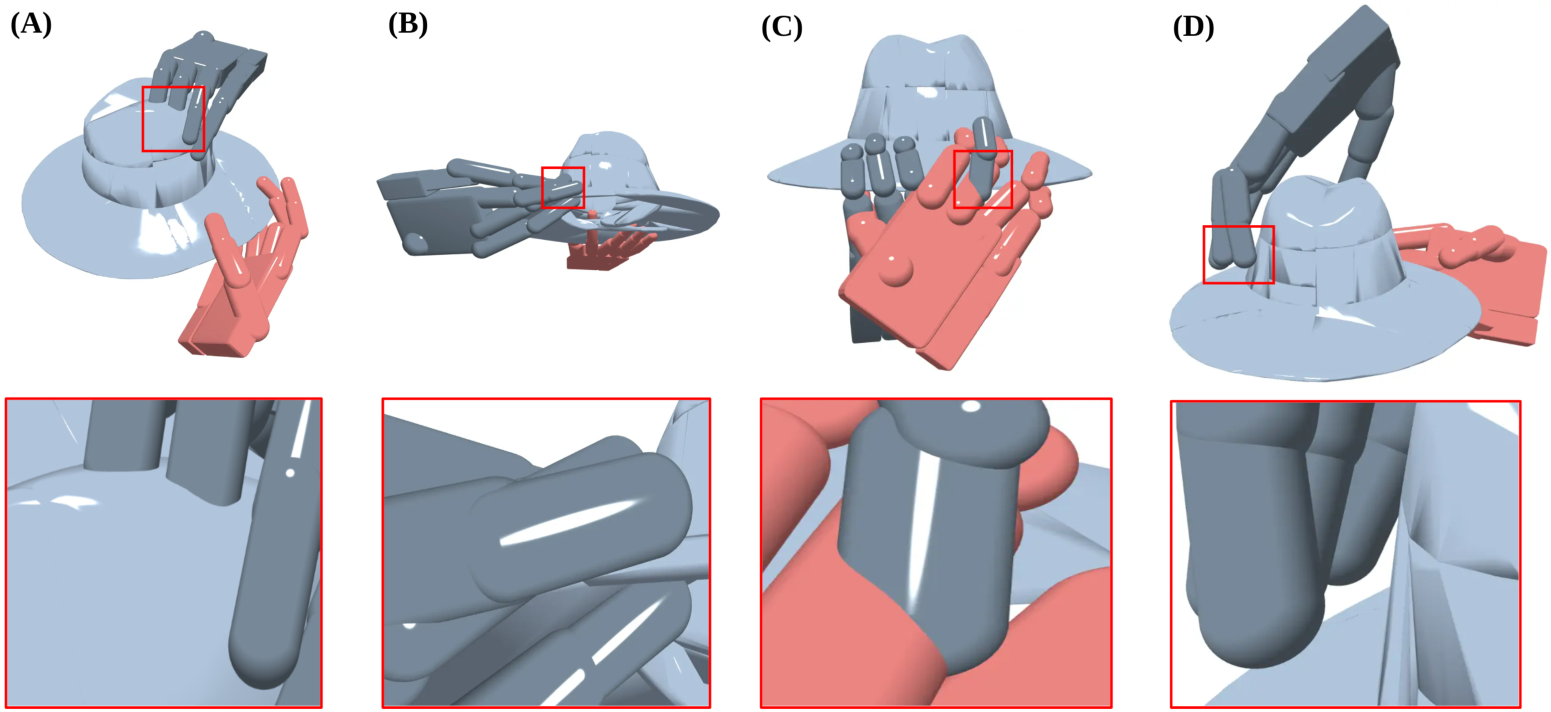
\includegraphics[width=0.86\columnwidth]{figs/selected/bimanual_grasp_penetration.png}
    \caption{Two failures of synthesised two-hand grasps, each enlarged at the
      contact: (A) a finger inside the object, (C) a finger inside the other hand.
      Both look plausible whole~\cite{bimangrasp_2024}.}
    \label{fig:bimanual-penetration}
    \licensed[panels (A) and (C) of Fig.~9]{Fig.~9 of Shao and Xiao, arXiv:2411.15903}{CC BY 4.0}{https://creativecommons.org/licenses/by/4.0/}
  \end{figure}}
}{}}{}
\makeatother

% A hand photograph at the head of the hardware section.
\providecommand{\plateLeapOverview}{}\plateLeapOverview


No degree-of-freedom, force, weight or price figure in Table~\ref{tab:hands-available} or
Table~\ref{tab:hands-announced}, both set in Appendix~\ref{app:tables}, was measured by anyone
outside the maker. Six rows are the exception, from peer-reviewed papers with stated protocols:
ILDA, Pisa/IIT, ORCA, RUKA, LEAP and BiDexHand. Every other claim is dated at its source.
Table~\ref{tab:hands-announced} prints the date beside each announced hand, and the dates for the
hands that can be bought are in the repository tabulation
(\texttt{paper/tables/table2\_hands\_available.md}, the \emph{claim date} column), which runs from
Shadow's specification of 4 December 2024 to vendor pages fetched on 17 September 2026.

The degree-of-freedom count is the first number a vendor states and the least comparable one.
Shadow's specification of 4 December 2024 reads ``20 actuated DOF and a further 4 under-actuated
movements for a total of 24 joints'' \cite{shadow_dexterous_hand_2005}. Table~\ref{tab:hands-available} prints joints first and
actuated DoF second, and the gap is the informative number. Where a vendor's own DoF figure
differs from the joint count, the joint count is what the table prints, as with Inspire's ``Degrees
of freedom 6, Numbers of joints 12'' \cite{inspire_rh56dfx_2023}. An actuator count is neither of those
two, and the repository tabulation keeps it in a column of its own. DexHand states no joint count at all, only 16 finger micro-servos and
two wrist servos, so 18 servos is the only count quotable for it \cite{dexhand_open_source_2023}. Daxo
states 120 actuators, no DoF figure, and a tendon structure with no rigid joints, which has far
fewer kinematic degrees of freedom than actuators \cite{daxo_muscle_v0_2025}.

% A transmission left exposed, beside the actuation-ratio argument.
\providecommand{\plateIldaLinkage}{}\plateIldaLinkage

The actuation ratio is the real decision. The Pisa/IIT SoftHand drives 19 joints from one motor and
its authors state the cost plainly: ``No in-hand dexterous manipulation is required for this
prototype'' \cite{pisa_iit_softhand_2014}. Tendon drive moves the motors off the fingers and the mass
follows them. Shadow's hand plus forearm weighs 4.3 kg, against 1.1 kg for the ILDA hand alone with
every motor in its palm \cite{shadow_dexterous_hand_2005,ilda_hand_2021}. ILDA states an 18 kg payload
against Shadow's 4 kg in a power grasp, and Shadow states no fingertip force at all. What tendons
cost is state estimation. The Faive Hand estimated joint angles from tendon length through a Kalman
filter and its cube reorientation failed on hardware, which its authors blamed on ``poor joint angle
measurement from the EKFs, especially when there is contact'' \cite{faive_hand_2023}. Ruka-v2 adds
detachable AS5600 encoders to measure that problem rather than close the loop on it, and those
encoders put its open-loop linear joint-to-motor map at 8.26 degrees of error over seven joints
\cite{ruka_v2_2026}.

% The linkage that cuts the actuator count, beside the coupling argument.
\providecommand{\plateCoupledLinkage}{}\plateCoupledLinkage

Direct drive trades torque density for transparency. LEAP's Dynamixel joints resist 19.5 N in a
pull-out test against the Allegro Hand's 8.5 N, at 595 g for the LEAP hand \cite{leap_hand_2023}, and
the Allegro's own weight has no reachable source. Linkage drive is the argument against the
forearm. ILDA puts 15 motors, drivers and ball screws inside the palm and reports 34 N at the
fingertip in the bent pose and 28 N stretched \cite{ilda_hand_2021}. Linkages buy coupling for free, as
in BiDexHand's four-bar that drives each DIP off its PIP, whose paper claims 16 actuated DoF and 21
joints while its README describes 15 servos driving 15 joints \cite{bidexhand_2025}.

Fingertip force is the number a hand buyer reads first, and across these rows it is six different
measurements. Table~\ref{tab:hands-available} puts the quantity beside the figure: pull-out resistance for
LEAP's 19.5 N, pinch for RUKA's 2.74 N and BrainCo's 15 N, fingertip normal force under a 1 cm
indenter for Unitree's 10 N, a calibrated five-trial fingertip force for BiDexHand's 2.14 N, a
peak vendor claim for 1X's 45 N, and two unlabelled spec columns for Sharpa's ``20 N \textbar{} 12 N''.
BrainCo's whole-fist grip of 50 N is a separate figure and is no longer in the same column as a
pinch. ORCA's 19.6 N was none of these. It is the newton equivalent of a 2 kg index-finger payload
at a fixed 600 mA motor current, so its force cell is empty and the figure is recorded as a payload
instead \cite{orca_hand_2025}. Payload is no more comparable than force, which is why
Table~\ref{tab:hands-available} does not print it. Nine of its twenty hands state one, in the
repository tabulation (\texttt{paper/tables/table2\_hands\_available.md}, the \emph{payload}
column), and no two state it under the same test: Shadow 4 kg in a power grasp with no protocol
given, Tesollo 2.5 kg pinching and 10 kg enveloping as rated figures, Unitree 3.5 kg palm-down and
4.5 kg palm-left on a 5 cm round object, ORCA 10.5 kg on four fingers and 2 kg on the index alone at
a fixed motor current, BiDexHand 4.54 kg lifted, and RUKA 6.0 kg as the weight at which its
joint-angle error passes 15 degrees.

Compliance is repairability seen twice over, and both are mechanical fuses: the Pisa/IIT
SoftHand's rolling-contact joints return to assembly after over-extension and ORCA's ``poppable''
pin joints dislocate rather than break \cite{pisa_iit_softhand_2014,orca_hand_2025}. ORCA also reports
tendon drive as maintenance: ``Prolonged use requires manual re-tensioning to maintain performance''.
What fails is rarely the motors. Its durability run found silicone skin degrading on two fingertips
after about 2,000 to 4,000 grasp cycles and sensor wires snapping on three after about 4,500 to
7,000. The sensing wore out an order of magnitude sooner than the hand.

Two properties matter before any of the above, and neither is a column of
Table~\ref{tab:hands-available}: both are in the repository tabulation, which prints a
\emph{control rate} and a \emph{URDF or MJCF} column for every row
(\texttt{paper/tables/table2\_hands\_available.md}). The first is the rate a loop can be
closed at, which spans 250 Hz on a Tesollo to 1 kHz on a Shadow, a Unitree or a Wuji, with the
Allegro at 333 Hz on its own CAN clock and Inspire stating no rate at all. LEAP's 500 Hz is a
serial query ceiling and its own sim-to-real policy runs at 20 Hz, which answer different questions
\cite{leap_hand_2023}. A reader deploying torque control is bitten by that first. The second is
whether a URDF or MJCF exists and who ships it, which is the bridge to Section~\ref{sec:simulators} and to this
survey's recommendation to pick a hand a simulator already carries. Shadow, Sharpa, Wuji, the
Ability Hand, RUKA, Faive and the Allegro driver ship one. LEAP is the warning: its paper says the
URDF is released and the released API repository contains none \cite{leap_hand_2023}.

% ---------------------------------------------------------------------------
% Table 2, the hands that can be bought or built, is set in Appendix B rather than here. It is
% consulted rather than read, so it is reference material; see the head of Appendix B.
% ---------------------------------------------------------------------------

\subsection{The hands the research literature actually runs on}
\label{sec:hands:used}

% ---------------------------------------------------------------------------
% Figure 2. The bar chart is wider than a column at its natural size, so it is
% scaled to the column rather than left to overflow.
% ---------------------------------------------------------------------------
\begin{figure}[!t]
  \centering
  \resizebox{\columnwidth}{!}{% generated by tools/make_tikz_figures.py; do not edit
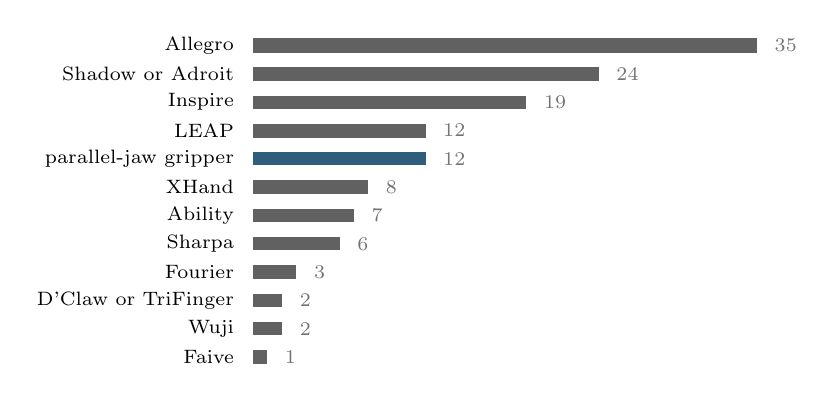
\begin{tikzpicture}[
  font=\footnotesize,
  bar/.style={draw=none,fill=black!62},
  barlight/.style={draw=none,fill=black!22},
  baracc/.style={draw=none,fill=accent},
  box/.style={draw=black!45,line width=0.3pt,inner sep=3pt,align=left},
  ghost/.style={draw=black!35,line width=0.3pt,dash pattern=on 1.4pt off 1.4pt,inner sep=3pt,align=left},
  lnk/.style={draw=black!38,line width=0.28pt},
  lbl/.style={font=\scriptsize},
  num/.style={font=\scriptsize\color{black!55}},
]

\node[lbl,anchor=east] at (0,-0.00) {Allegro};
\fill[bar] (0.12,-0.09) rectangle (6.52,0.09);
\node[num,anchor=west] at (6.62,-0.00) {35};
\node[lbl,anchor=east] at (0,-0.36) {Shadow or Adroit};
\fill[bar] (0.12,-0.45) rectangle (4.51,-0.27);
\node[num,anchor=west] at (4.61,-0.36) {24};
\node[lbl,anchor=east] at (0,-0.72) {Inspire};
\fill[bar] (0.12,-0.80) rectangle (3.59,-0.64);
\node[num,anchor=west] at (3.69,-0.72) {19};
\node[lbl,anchor=east] at (0,-1.08) {LEAP};
\fill[bar] (0.12,-1.17) rectangle (2.31,-1.00);
\node[num,anchor=west] at (2.41,-1.08) {12};
\node[lbl,anchor=east] at (0,-1.44) {parallel-jaw gripper};
\fill[baracc] (0.12,-1.52) rectangle (2.31,-1.35);
\node[num,anchor=west] at (2.41,-1.44) {12};
\node[lbl,anchor=east] at (0,-1.80) {XHand};
\fill[bar] (0.12,-1.88) rectangle (1.58,-1.71);
\node[num,anchor=west] at (1.68,-1.80) {8};
\node[lbl,anchor=east] at (0,-2.16) {Ability};
\fill[bar] (0.12,-2.24) rectangle (1.40,-2.07);
\node[num,anchor=west] at (1.50,-2.16) {7};
\node[lbl,anchor=east] at (0,-2.52) {Sharpa};
\fill[bar] (0.12,-2.60) rectangle (1.22,-2.43);
\node[num,anchor=west] at (1.32,-2.52) {6};
\node[lbl,anchor=east] at (0,-2.88) {Fourier};
\fill[bar] (0.12,-2.96) rectangle (0.67,-2.79);
\node[num,anchor=west] at (0.77,-2.88) {3};
\node[lbl,anchor=east] at (0,-3.24) {D'Claw or TriFinger};
\fill[bar] (0.12,-3.32) rectangle (0.49,-3.15);
\node[num,anchor=west] at (0.59,-3.24) {2};
\node[lbl,anchor=east] at (0,-3.60) {Wuji};
\fill[bar] (0.12,-3.68) rectangle (0.49,-3.51);
\node[num,anchor=west] at (0.59,-3.60) {2};
\node[lbl,anchor=east] at (0,-3.96) {Faive};
\fill[bar] (0.12,-4.04) rectangle (0.30,-3.87);
\node[num,anchor=west] at (0.40,-3.96) {1};
\end{tikzpicture}}
  \caption{Which hands the literature actually runs on. Per hand, the number of method papers
  whose own experiments use it. Of 112 method rows, 103 name a hand, and a paper
  using two hands is counted under both. The accented bar is the parallel-jaw gripper, which is
  not a dexterous hand, and only three dexterous hands carry more method rows than it. The Adroit
  is the MuJoCo model of a Shadow hand and takes a line of its own, three of whose four rows name
  no Shadow, so the Shadow bar is the rows that name a Shadow itself. Only
  hands with at least one method row appear, so the nine company-announced hands of
  Table~\ref{tab:hands-announced} and the hands of Table~\ref{tab:hands-available}
  that no paper runs on are absent from the chart.}
  \label{fig:hands}
\end{figure}

% Research hands photographed to scale, beside the count of who runs on what.
\providecommand{\plateHandScale}{}\plateHandScale

The two oldest designs in Table~\ref{tab:hands-available} carry 49 of the 103 method rows that name a hand at all, and
seven rows use both. Neither design's date is confirmed by its own sources, so 2005 and 2016 are
the bibliography's. \figurename~\ref{fig:hands} counts, per hand, the method papers whose own experiments use it. Of
112 method rows, 103 name a hand. The Allegro accounts for 35, Shadow for 21, the Inspire RH56
family for 19, a parallel-jaw gripper for 12 and LEAP for 12. Seventy-five of the 103 name an
Allegro, a Shadow or Adroit model, LEAP or an Inspire.

The Allegro's position is the uncomfortable part. Its product page at allegrohand.com/v4 returned
HTTP 404 while the Wonik wiki timed out \cite{allegro_hand_v4_2016}. Everything Table~\ref{tab:hands-available} confirms about
the most-used hand in the corpus comes from its ROS driver: 16 joints, four fingers, a torque
interface, a 333 Hz CAN clock, 12 V, no tactile sensing. Its weight, joint torque, payload and
price have no reachable source. The field's most common platform cannot be specified from a page a
reader can open.

Concentration would matter less if the hand did not move the result, and it does. On the same
simulated cube rotation, LEAP reaches 0.2288 rad/s against the Allegro's 0.0828 rad/s
\cite{leap_hand_2023}, and RUKA reports a 2.74 N pinch against the Allegro's 1.60 N under the same
three-trial pinch test \cite{ruka_2025}. A method compared only on Allegro hardware is compared at one
point in a space where a single axis moves the headline number two or three times over. Two further
patterns follow. Inspire, XHand and Sharpa take 29 of the 103 rows between them, four rows use two
of the three, and none is earlier than 2024. Eight take none at all: ORCA, RUKA, Ruka-v2,
BiDexHand, DexHand, the Proception ProHand, the Tesollo DG-5F and the Unitree Dex5.

\subsection{Open hardware and the collapse in cost}
\label{sec:hands:open}

Six rows in Table~\ref{tab:hands-available} are open hardware, and LEAP Hand V2 in
Table~\ref{tab:hands-announced} is a seventh. Five of the seven state a dollar cost: \$2,000 for
LEAP, \$3,000 for LEAP Hand V2, \$1,500 for Ruka-v2, \$1,300 for RUKA and \$300 for DexHand. ORCA
states a material cost below 2,000 CHF that the price column leaves unconverted, and BiDexHand
states none \cite{orca_hand_2025,bidexhand_2025}. The Faive Hand states neither a cost nor a licence that could be
read, so it is not counted as open hardware here \cite{faive_hand_2023}. Two of the stated bases need
saying. DexHand's \$300 is ``additional total cost of components'', excluding the printing and the
wrist servos \cite{dexhand_open_source_2023}, and ORCA's own figure sits against Ruka-v2's table listing
ORCA at about \$3.5K \cite{ruka_v2_2026}.

The expensive end of the collapse is secondhand throughout. The only six-figure numbers on disk are
RUKA's comparison table at \$100,000 for a Shadow Hand and Faive's ``steep price tag of 110k GBP''
\cite{ruka_2025,faive_hand_2023}. Shadow's own page says to discuss pricing and Table~\ref{tab:hands-available}'s price cell
for it is empty. The collapse is real at the cheap end and secondhand at the expensive one, and it
has barely moved the literature. Twelve of the 103 hand-naming method rows use an open-hardware
hand, and all twelve are LEAP.

What the cheap hands give up is sensing. LEAP has none and names touch sensors as future work
\cite{leap_hand_2023}, RUKA states its design ``lacks tactile sensing'' \cite{ruka_2025}, and BiDexHand's
sources never mention touch \cite{bidexhand_2025}. ORCA is the exception, with binary FSR fingertips
whose threshold was measured as low as 0.05 N on a fresh fingertip, against the sensor's rated
0.29 N, and 6.38 N on a degraded one \cite{orca_hand_2025}.

\subsection{Announced and unreleased hands}
\label{sec:hands:announced}

Behind Table~\ref{tab:hands-announced}'s rows sit three kinds of evidence, and conflating them is how a DoF figure with no
source ends up in a survey. Vendor prose carrying numbers is the strongest, as on 1X's page of
9 July 2026 \cite{onex_neo_hand_2026}. Video is second and carries none. Press or bibliography assertion
is third, as with Tesla's V3 hand, known here only through a paraphrase of patents because the
USPTO PDF parsed empty \cite{tesla_optimus_hand_2025}. Table~\ref{tab:hands-announced} blanks the cells resting on the third
class and footnotes who did the arithmetic.

A survey can go one step past recording that a claim is unverified, which is to say which claims
are implausible on their face. Daxo's 120 actuators in 750 g is about 6 g per actuator including
structure, tendons, routing and skin \cite{daxo_muscle_v0_2025}. Clone's 27 degrees of freedom under
2 pounds excludes a 500 W pump the source does not confirm is excluded \cite{clone_robotics_hand_2024}.
Figure 03's ``Degrees of freedom, hands \textbar{} 20'' sits on the same tracker page as ``Number of fingers \textbar{}
10'', so it is almost certainly the pair \cite{figure_03_hand_2025}. Tesla's repeated 22 is one article's
arithmetic of four DoF on each of five fingers plus two at the wrist, and Gen 2's own figure was 11
\cite{tesla_optimus_hand_2025}.

Scepticism belongs to the evidence class, not to which table a row lands in. Sharpa's 22 of 22,
Wuji's 20 of 20 and Tesollo's 20 of 20 are vendor claims about unmeasured hardware and they sit in
Table~\ref{tab:hands-available}, where Sharpa's page footnotes ``Specifications may vary between products'' and Wuji's says
the spec ``will continue to iterate'' on a Beta1 product \cite{sharpa_wave_2026,wuji_hand_2025}. Even
the best-specified vendor page in the corpus leaves its fingertip-force columns unlabelled.

% ---------------------------------------------------------------------------
% Table 3, the announced and unreleased hands, is set in Appendix B rather than here.
% ---------------------------------------------------------------------------

\subsection{Tactile sensing as part of the hand}
\label{sec:hands:tactile}

% Vision-based tactile sensors used as the fingertips themselves.
\providecommand{\plateDigitFingertips}{}\plateDigitFingertips

DIGIT set the cost floor. It is 20 by 27 by 18 mm, weighs about 20 g, streams 640x480 at 60 fps,
and its paper states a ``total estimated manufacturing cost is approximately 15 USD per sensor ...
when manufactured in a batch of 1000'' \cite{digit_2020}. Durability was as much the contribution as
price: its gel degraded 0.3 percent over 15 abrasion passes, against 805 and 918 percent for the
two gels compared with it.

Digit 360 is the same lineage at a different operating point, claiming about 8.3 million taxels,
spatial features to 7 um, normal and shear force resolution of 1.01 mN and 1.27 mN, and on-device
processing that cuts event-to-action latency from 6 ms to 1.2 ms \cite{digit360_2024}. It is also not
for sale, and no corpus paper's parsed text names it.

% A pad fitted to a commercial hand: the other way to change what a fingertip does.
\providecommand{\plateInspireTactilePad}{}\plateInspireTactilePad

XELA's uSkin is the non-camera alternative and the one that bolts onto hands the field already
uses. Its curved fingertip kit for the Allegro V4 and LEAP carries 30 three-axis sensing points, a
full Allegro integration reaches 368, resolution is 0.1 gram-force, and the kit runs at 275 Hz
\cite{xela_uskin_2020}. The 500 Hz figure often quoted belongs to the product family, not the curved
fingertip. One corpus paper names it, \cite{sparsh_2024}, whose self-supervised encoders are pre-trained
on 462.7k tactile images and beat matched end-to-end models by 95.1 percent when both see 33 to 50
percent of the labels. Its own bead-maze policies never complete the maze on the real robot.

The usage number is the one to keep, and it needs its inclusion rule stated: a sensor physically on
the hand, read by the deployed policy. Eight of 112 method rows meet it: \cite{anyrotate_2024,articulated_tools_inhand_2025,dexteleop0_2026,dexumi_2025,hato_visuotactile_2024,robot_synesthesia_2023,rotateit_2023} and \cite{rotating_without_seeing_2023}. The rule excludes
\cite{penspin_2024}, whose 20 binary contacts are simulated on an Allegro that has no tactile hardware
and whose released config sets \texttt{enable\_tactile: False}, and it excludes \cite{dexndm_2025} and
\cite{dexplore_2025} for the same reason. Sixty-five of the 112 method papers mention tactile sensing
somewhere, which is the gap worth quoting. Thirty-five is the count over this survey's notes.

Almost none of the eight uses a high-resolution sensor. Yin et al.
\cite{rotating_without_seeing_2023} remove vision entirely and rotate objects from 16 binary touch
sensors over the palm, links and fingertips, deployed zero-shot to a real Allegro, and Robot
Synesthesia uses 16 force-sensing resistors read as binary \cite{robot_synesthesia_2023}. Two papers
exclude touch deliberately, HORA reporting rotation ``even without the usage of vision and tactile
sensing'' \cite{hora_2022}, and ORCA's authors dropping it from their reinforcement learning ``due
to the additional complexity involved in accurately modeling them'' \cite{orca_hand_2025}. Taxel
counts have risen by three orders of magnitude while the policies consuming them have stayed at
binary contact.

\subsection{What is sold against what is published on}
\label{sec:hands:gap}

The hands missing from \figurename~\ref{fig:hands} carry the finding. None of the nine company-announced hands in Table~\ref{tab:hands-announced}
appears in a single method row whose own experiments use it. Tesla, Figure, 1X, Sanctuary, Boston
Dynamics, Xiaomi, Clone, Daxo and PaXini account for zero of the 112 method papers' experiments.
The nearest thing to a counterexample is \cite{helix_2025}, a Figure blog post claiming a 35-DoF
whole-upper-body action space at 200 Hz that includes individual finger control. It never names the
hand, gives no per-hand DoF count, and reports no success rate or trial count for any task. It is
the maker describing its own unreleased hand, which is the evidence class the finding is about. The
four research prototypes in Table~\ref{tab:hands-announced} are in a different position, since the Faive Hand and LEAP Hand
v2 Advanced account for three method rows between them \cite{graspxl_2024,bidex_teleop_2024}.

Table~\ref{tab:hands-announced}'s emptiness is measurable and part of the same finding. Over the
eight specification columns it prints, from DoF to price, 58 percent of its cells are values no
source stated, against 42 percent for the hands that can be bought; both captions state their own
count. Over the twelve specification columns the repository tabulation carries, the same split is 61
to 39. The hands with the highest advertised DoF counts have the least specification behind
them.

The one hand that crosses the gap crosses it because its maker published rather than announced.
ByteDexter reaches a method row through a ByteDance technical report stating 21 DoF per hand, 16
piezoresistive fingertip channels in the action vector and real-robot success rates
\cite{gr_dexter_2025}, not through a product page. That mechanism is available to every vendor in
Table~\ref{tab:hands-announced} and none has used it.

The gap runs the other way too, and the last column of Table~\ref{tab:hands-available} shows it. Eight hands that can be bought
or built from published designs take zero method rows each: the Unitree Dex5 with 94 pressure
sensors on its P variant \cite{unitree_dex5_2025}, the fully actuated Tesollo DG-5F
\cite{tesollo_dg5f_2024}, the 22-DoF Proception ProHand \cite{proception_prohand_2026}, ORCA, RUKA,
Ruka-v2, BiDexHand and DexHand. Cheapness is established only for RUKA, Ruka-v2 and DexHand,
because Table~\ref{tab:hands-available}'s price cell is empty for Unitree, Tesollo, the ProHand,
ORCA and BiDexHand, and the only Dex5
price on disk is Ruka-v2's secondhand ``\textasciitilde{}\$25K'' \cite{ruka_v2_2026}. A reader choosing a hand on this
corpus's evidence has two well-precedented options, an Allegro or an Inspire, and a third in LEAP
if twelve papers is enough. Everything else is a press release or a hand nobody has published on.

\input{sections/04_simulators}
%% Section 5, How policies are trained. Converted from paper/sections/05_training.md.
\section{Training a dexterous policy}
\label{sec:training}

\subsection{Sources of supervision}
\label{sec:train:space}

% --- the one reproduced plate in this section -------------------------------
% Three reproduced plates survive in the whole paper; one of them is here. Load
% tex/figs/plates.tex if nothing has loaded it already. The \providecommand
% before the call makes a missing plate an empty command rather than an error.
% Read tex/PERMISSIONS.md before posting.
% ---------------------------------------------------------------------------
\makeatletter
\@ifundefined{plateRetargetArtifacts}{\IfFileExists{figs/plates.tex}{% The one reproduced plate.
% Rebuilt from its source PDF by tools/relayout_plates.py; see tex/figs/SELECTED.md for the crop
% box and tex/PERMISSIONS.md for the licence it is used under.
%
% A plate is kept only where a photograph or a render carries something a drawing cannot, and
% only where the paper has the right to print it without asking anyone. Everything else that was
% reproduced has been redrawn in the paper's own style (figs/fig_transmission, fig_collision,
% fig_tactiledepth, fig_contactlabel, fig_retarget) or dropped, because the prose already made the
% point or because no honest drawing could be made from what the corpus records. That took
% eighteen plates to one, eleven visual styles to four, and eleven open permissions to none.
%
% The survivor is single column and single panel. It is not a `figure*`: a borrowed plate has not
% earned the page width.
%
% One command for it. A section author places it by writing
%   \plateGraspPenetration
% at the point in the section where the float should be anchored, once: a plate called twice
% prints twice, on two pages, under two numbers.
%
% The plate credits its source inside its own caption with \src or \cite, and carries \licensed as
% well, because its source is CC BY 4.0 and the licence asks for an attribution line.

% ========================================================== Sec. VI, two hands

\newcommand{\plateGraspPenetration}{%
  \begin{figure}[t]
    \centering
    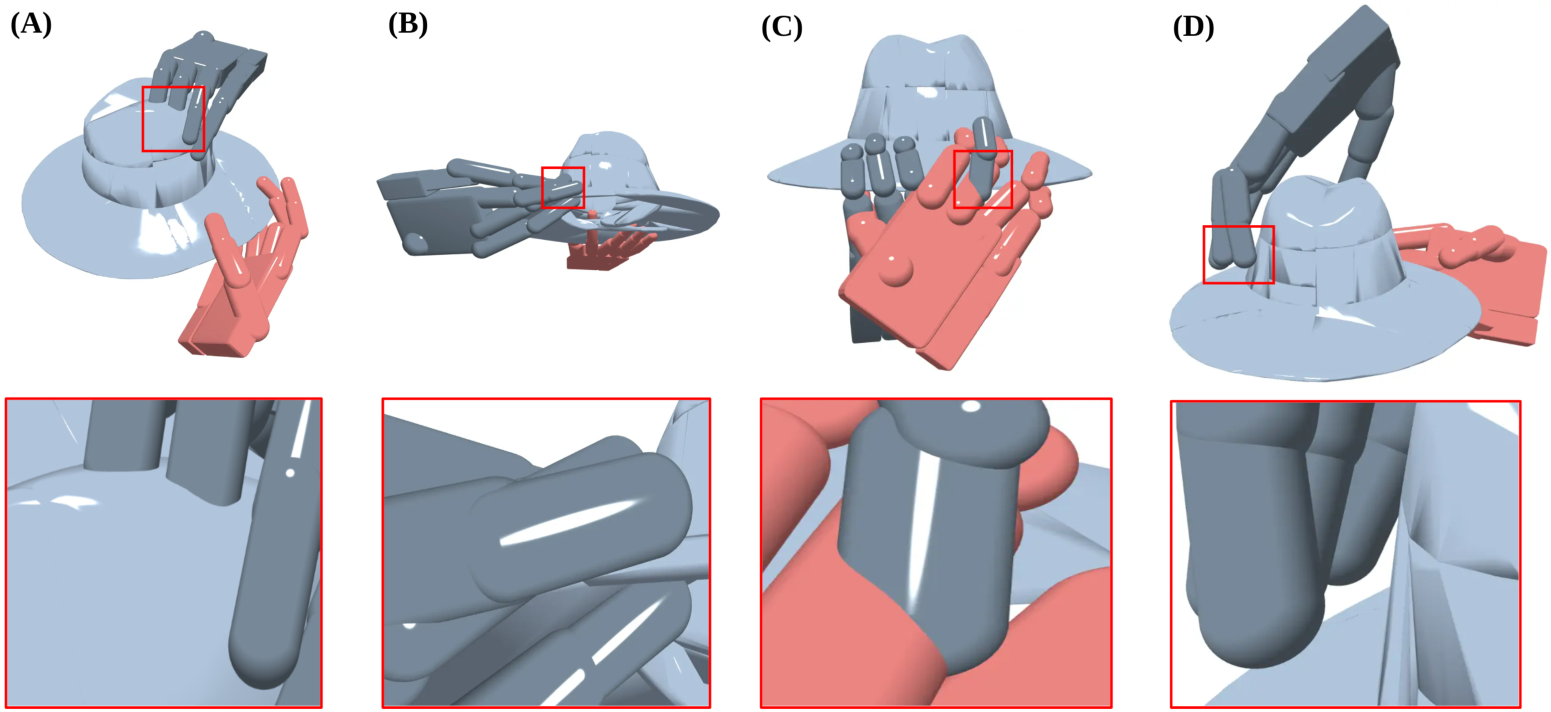
\includegraphics[width=0.86\columnwidth]{figs/selected/bimanual_grasp_penetration.png}
    \caption{Two failures of synthesised two-hand grasps, each enlarged at the
      contact: (A) a finger inside the object, (C) a finger inside the other hand.
      Both look plausible whole~\cite{bimangrasp_2024}.}
    \label{fig:bimanual-penetration}
    \licensed[panels (A) and (C) of Fig.~9]{Fig.~9 of Shao and Xiao, arXiv:2411.15903}{CC BY 4.0}{https://creativecommons.org/licenses/by/4.0/}
  \end{figure}}
}{}}{}
\makeatother

A dexterous policy is defined by what supervises it, and four sources are in use across the
corpus's 112 method rows: a reward function supervises reinforcement learning, a human
demonstration supervises imitation, a human reference trajectory supervises a physics-based
tracker, which is imitation with a simulator in the loop, and nothing supervises a model-based
planner, which is handed a cost and a model instead.

The labels do not partition the corpus. Of the 112 method rows, 53 are tagged reinforcement
learning, 27 behaviour cloning, 23 distillation, 18 generalist or vision-language-action, 14
teleoperation systems, 14 diffusion, 10 data collection, 8 flow matching, 6 reinforcement learning
from demonstrations, 6 trajectory optimisation, 5 model-predictive control, 4 grasp synthesis and
2 world models. The tags sum to far more than 112 because most methods published since 2024 sit on
two branches at once. \figurename~\ref{fig:taxonomy} draws the tree and the cross-links. The
repository carries the row-by-row version of the same thing, one row per method, and that is what
to scan when looking for work comparable to your own.

What the deployed policy looks like once training is done matters more than the name a paper gives
itself, and on that axis the field has converged hard. Section~\ref{sec:train:hybrids} shows why.

\textbf{What the tabulation does not record.}\label{sec:train:master}
The emptiest columns of the method tabulation are the ones a reader most needs: only 31 rows state
an environment count, only 70 state how many real trials are behind the headline number, and only
39 state how many unseen objects were tested. The trial and unseen-object figures are the audited
ones, after Section~\ref{subsec:reporting} recovered 15 trial counts and 7 unseen-object counts that
the notes carried and the extraction had dropped. A mostly empty row is not a weak method, but it is
one that cannot be compared with any other row here. All 112 rows carry the columns this survey
reads, and Appendix~\ref{app:method} says where they are and how to read them.

\begin{figure*}[!t]
  \centering
  \IfFileExists{figs/fig_taxonomy.tex}{% Figure: what supervises a dexterous policy. Drawn for the LaTeX edition in the restrained
% palette: greyscale plus the one accent, thin rules, square corners, document font. It redraws
% paper/figures/fig4_taxonomy.svg to the specification carried in paper/sections/05_training.md.
% Every count is the number of corpus method rows the leaf's stated predicate selects, recomputed
% from corpus/rows/*.json with the predicates of tools/make_flow_tree.py, so no leaf claims more
% than it tests: the PPO leaves read `algorithm` and `sim` rather than the RL tag, the reward
% branch counts RL and RL+demo together, the demonstration branch counts the union of BC,
% diffusion and flow, and the no-learning branch counts the three papers that learn no policy
% rather than the eleven rows carrying a trajopt or MPC tag. A paper may appear at more than one
% leaf. Bars are linear in the count. Designed for a two-column figure* at 18.1 cm.
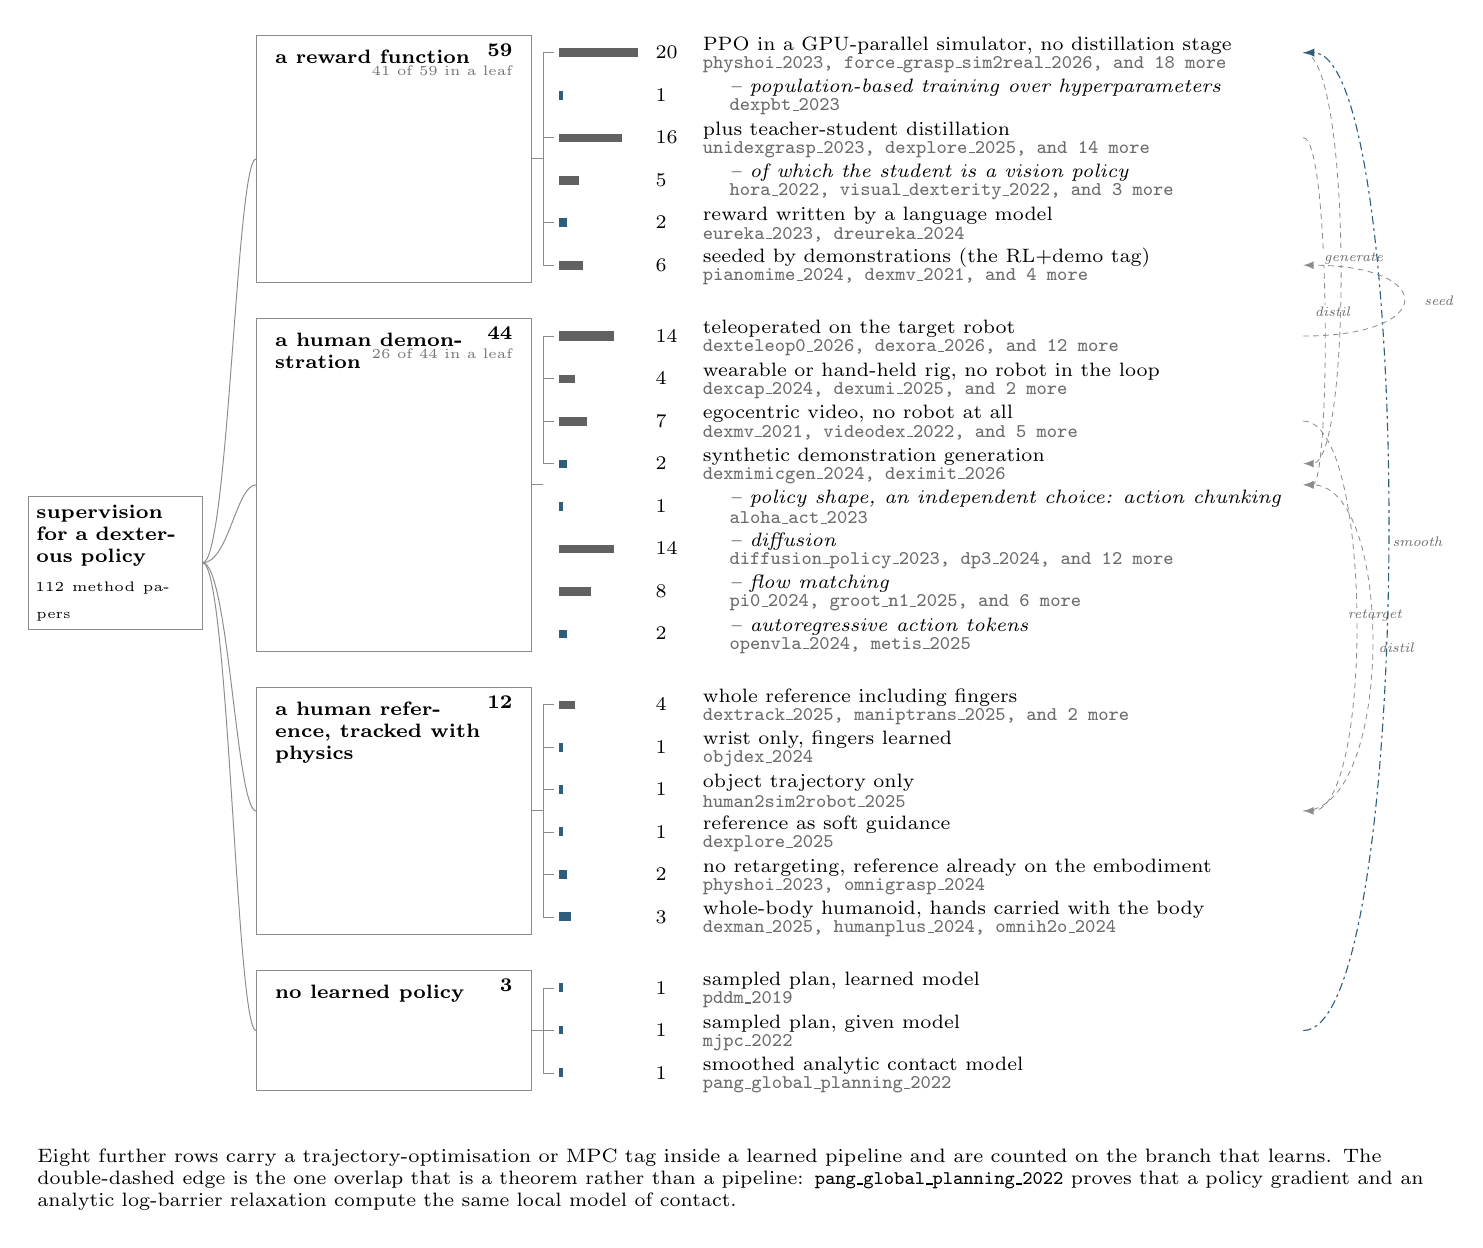
\begin{tikzpicture}[
  font=\footnotesize,
  bar/.style={draw=none,fill=black!62},
  baracc/.style={draw=none,fill=accent},
  box/.style={draw=black!45,line width=0.3pt,inner sep=3pt,align=left},
  tree/.style={draw=black!45,line width=0.35pt},
  lnk/.style={draw=black!38,line width=0.28pt},
  lbl/.style={font=\scriptsize,anchor=west},
  ann/.style={font=\scriptsize\itshape,anchor=west},
  key/.style={font=\scriptsize\ttfamily\color{black!58},anchor=west},
  num/.style={font=\scriptsize,anchor=west},
  bname/.style={font=\scriptsize\bfseries,anchor=north west,align=left,text width=2.7cm},
  xl/.style={draw=black!45,line width=0.3pt,dash pattern=on 2pt off 1.6pt,-latex},
  xt/.style={draw=accent,line width=0.4pt,dash pattern=on 3pt off 1.4pt on 1pt off 1.4pt,-latex},
  xw/.style={font=\tiny\itshape\color{black!58},fill=white,inner sep=0.6pt},
  ftr/.style={font=\scriptsize,anchor=north west,align=left,text width=17.6cm},
]
\node[box,anchor=west,text width=2.0cm] (root) at (0,-6.48) {\scriptsize\textbf{supervision for a dexterous policy}\\[1pt]{\tiny 112 method papers}};
\draw[box] (2.90,0.22) rectangle (6.40,-2.92);
\node[bname] at (3.02,0.16) {a reward function};
\node[num,anchor=east,font=\scriptsize\bfseries] at (6.28,0.03) {59};
\node[anchor=east,font=\tiny\color{black!55}] at (6.28,-0.23) {41 of 59 in a leaf};
\draw[tree] (root.east) .. controls (2.55,-6.48) and (2.65,-1.35) .. (2.90,-1.35);
\draw[tree] (6.55,0.00) -- (6.55,-2.70);
\draw[tree] (6.40,-1.35) -- (6.55,-1.35);
\draw[tree] (6.55,0.00) -- (6.69,0.00);
\draw[tree] (6.55,-1.08) -- (6.69,-1.08);
\draw[tree] (6.55,-2.16) -- (6.69,-2.16);
\draw[tree] (6.55,-2.70) -- (6.69,-2.70);
\draw[box] (2.90,-3.38) rectangle (6.40,-7.60);
\node[bname] at (3.02,-3.44) {a human demonstration};
\node[num,anchor=east,font=\scriptsize\bfseries] at (6.28,-3.57) {44};
\node[anchor=east,font=\tiny\color{black!55}] at (6.28,-3.83) {26 of 44 in a leaf};
\draw[tree] (root.east) .. controls (2.55,-6.48) and (2.65,-5.49) .. (2.90,-5.49);
\draw[tree] (6.55,-3.60) -- (6.55,-5.22);
\draw[tree] (6.40,-5.49) -- (6.55,-5.49);
\draw[tree] (6.55,-3.60) -- (6.69,-3.60);
\draw[tree] (6.55,-4.14) -- (6.69,-4.14);
\draw[tree] (6.55,-4.68) -- (6.69,-4.68);
\draw[tree] (6.55,-5.22) -- (6.69,-5.22);
\draw[box] (2.90,-8.06) rectangle (6.40,-11.20);
\node[bname] at (3.02,-8.12) {a human reference, tracked with physics};
\node[num,anchor=east,font=\scriptsize\bfseries] at (6.28,-8.25) {12};
\draw[tree] (root.east) .. controls (2.55,-6.48) and (2.65,-9.63) .. (2.90,-9.63);
\draw[tree] (6.55,-8.28) -- (6.55,-10.98);
\draw[tree] (6.40,-9.63) -- (6.55,-9.63);
\draw[tree] (6.55,-8.28) -- (6.69,-8.28);
\draw[tree] (6.55,-8.82) -- (6.69,-8.82);
\draw[tree] (6.55,-9.36) -- (6.69,-9.36);
\draw[tree] (6.55,-9.90) -- (6.69,-9.90);
\draw[tree] (6.55,-10.44) -- (6.69,-10.44);
\draw[tree] (6.55,-10.98) -- (6.69,-10.98);
\draw[box] (2.90,-11.66) rectangle (6.40,-13.18);
\node[bname] at (3.02,-11.72) {no learned policy};
\node[num,anchor=east,font=\scriptsize\bfseries] at (6.28,-11.85) {3};
\draw[tree] (root.east) .. controls (2.55,-6.48) and (2.65,-12.42) .. (2.90,-12.42);
\draw[tree] (6.55,-11.88) -- (6.55,-12.96);
\draw[tree] (6.40,-12.42) -- (6.55,-12.42);
\draw[tree] (6.55,-11.88) -- (6.69,-11.88);
\draw[tree] (6.55,-12.42) -- (6.69,-12.42);
\draw[tree] (6.55,-12.96) -- (6.69,-12.96);
\fill[bar] (6.75,-0.06) rectangle (7.75,0.06);
\node[num] at (7.85,0.00) {20};
\node[lbl] at (8.45,0.09) {PPO in a GPU-parallel simulator, no distillation stage};
\node[key] at (8.45,-0.15) {physhoi\_2023, force\_grasp\_sim2real\_2026, and 18 more};
\fill[baracc] (6.75,-0.60) rectangle (6.80,-0.49);
\node[num] at (7.85,-0.54) {1};
\node[ann] at (8.79,-0.45) {-- population-based training over hyperparameters};
\node[key] at (8.79,-0.69) {dexpbt\_2023};
\fill[bar] (6.75,-1.14) rectangle (7.55,-1.03);
\node[num] at (7.85,-1.08) {16};
\node[lbl] at (8.45,-0.99) {plus teacher-student distillation};
\node[key] at (8.45,-1.23) {unidexgrasp\_2023, dexplore\_2025, and 14 more};
\fill[bar] (6.75,-1.68) rectangle (7.00,-1.57);
\node[num] at (7.85,-1.62) {5};
\node[ann] at (8.79,-1.53) {-- of which the student is a vision policy};
\node[key] at (8.79,-1.77) {hora\_2022, visual\_dexterity\_2022, and 3 more};
\fill[baracc] (6.75,-2.22) rectangle (6.85,-2.10);
\node[num] at (7.85,-2.16) {2};
\node[lbl] at (8.45,-2.07) {reward written by a language model};
\node[key] at (8.45,-2.31) {eureka\_2023, dreureka\_2024};
\fill[bar] (6.75,-2.76) rectangle (7.05,-2.65);
\node[num] at (7.85,-2.70) {6};
\node[lbl] at (8.45,-2.61) {seeded by demonstrations (the RL+demo tag)};
\node[key] at (8.45,-2.85) {pianomime\_2024, dexmv\_2021, and 4 more};
\fill[bar] (6.75,-3.66) rectangle (7.45,-3.54);
\node[num] at (7.85,-3.60) {14};
\node[lbl] at (8.45,-3.51) {teleoperated on the target robot};
\node[key] at (8.45,-3.75) {dexteleop0\_2026, dexora\_2026, and 12 more};
\fill[bar] (6.75,-4.20) rectangle (6.95,-4.09);
\node[num] at (7.85,-4.14) {4};
\node[lbl] at (8.45,-4.05) {wearable or hand-held rig, no robot in the loop};
\node[key] at (8.45,-4.29) {dexcap\_2024, dexumi\_2025, and 2 more};
\fill[bar] (6.75,-4.74) rectangle (7.10,-4.63);
\node[num] at (7.85,-4.68) {7};
\node[lbl] at (8.45,-4.59) {egocentric video, no robot at all};
\node[key] at (8.45,-4.83) {dexmv\_2021, videodex\_2022, and 5 more};
\fill[baracc] (6.75,-5.28) rectangle (6.85,-5.17);
\node[num] at (7.85,-5.22) {2};
\node[lbl] at (8.45,-5.13) {synthetic demonstration generation};
\node[key] at (8.45,-5.37) {dexmimicgen\_2024, deximit\_2026};
\fill[baracc] (6.75,-5.82) rectangle (6.80,-5.71);
\node[num] at (7.85,-5.76) {1};
\node[ann] at (8.79,-5.67) {-- policy shape, an independent choice: action chunking};
\node[key] at (8.79,-5.91) {aloha\_act\_2023};
\fill[bar] (6.75,-6.36) rectangle (7.45,-6.25);
\node[num] at (7.85,-6.30) {14};
\node[ann] at (8.79,-6.21) {-- diffusion};
\node[key] at (8.79,-6.45) {diffusion\_policy\_2023, dp3\_2024, and 12 more};
\fill[bar] (6.75,-6.90) rectangle (7.15,-6.79);
\node[num] at (7.85,-6.84) {8};
\node[ann] at (8.79,-6.75) {-- flow matching};
\node[key] at (8.79,-6.99) {pi0\_2024, groot\_n1\_2025, and 6 more};
\fill[baracc] (6.75,-7.44) rectangle (6.85,-7.33);
\node[num] at (7.85,-7.38) {2};
\node[ann] at (8.79,-7.29) {-- autoregressive action tokens};
\node[key] at (8.79,-7.53) {openvla\_2024, metis\_2025};
\fill[bar] (6.75,-8.34) rectangle (6.95,-8.23);
\node[num] at (7.85,-8.28) {4};
\node[lbl] at (8.45,-8.19) {whole reference including fingers};
\node[key] at (8.45,-8.43) {dextrack\_2025, maniptrans\_2025, and 2 more};
\fill[baracc] (6.75,-8.88) rectangle (6.80,-8.77);
\node[num] at (7.85,-8.82) {1};
\node[lbl] at (8.45,-8.73) {wrist only, fingers learned};
\node[key] at (8.45,-8.97) {objdex\_2024};
\fill[baracc] (6.75,-9.41) rectangle (6.80,-9.30);
\node[num] at (7.85,-9.36) {1};
\node[lbl] at (8.45,-9.27) {object trajectory only};
\node[key] at (8.45,-9.51) {human2sim2robot\_2025};
\fill[baracc] (6.75,-9.95) rectangle (6.80,-9.84);
\node[num] at (7.85,-9.90) {1};
\node[lbl] at (8.45,-9.81) {reference as soft guidance};
\node[key] at (8.45,-10.05) {dexplore\_2025};
\fill[baracc] (6.75,-10.49) rectangle (6.85,-10.38);
\node[num] at (7.85,-10.44) {2};
\node[lbl] at (8.45,-10.35) {no retargeting, reference already on the embodiment};
\node[key] at (8.45,-10.59) {physhoi\_2023, omnigrasp\_2024};
\fill[baracc] (6.75,-11.03) rectangle (6.90,-10.92);
\node[num] at (7.85,-10.98) {3};
\node[lbl] at (8.45,-10.89) {whole-body humanoid, hands carried with the body};
\node[key] at (8.45,-11.13) {dexman\_2025, humanplus\_2024, omnih2o\_2024};
\fill[baracc] (6.75,-11.93) rectangle (6.80,-11.82);
\node[num] at (7.85,-11.88) {1};
\node[lbl] at (8.45,-11.79) {sampled plan, learned model};
\node[key] at (8.45,-12.03) {pddm\_2019};
\fill[baracc] (6.75,-12.47) rectangle (6.80,-12.36);
\node[num] at (7.85,-12.42) {1};
\node[lbl] at (8.45,-12.33) {sampled plan, given model};
\node[key] at (8.45,-12.57) {mjpc\_2022};
\fill[baracc] (6.75,-13.01) rectangle (6.80,-12.90);
\node[num] at (7.85,-12.96) {1};
\node[lbl] at (8.45,-12.87) {smoothed analytic contact model};
\node[key] at (8.45,-13.11) {pang\_global\_planning\_2022};
\draw[xl] (16.20,-1.08) .. controls (16.55,-1.08) and (16.55,-5.49) .. (16.20,-5.49);
\node[xw] at (16.57,-3.29) {distil};
\draw[xl] (16.20,0.00) .. controls (16.82,0.00) and (16.82,-5.22) .. (16.20,-5.22);
\node[xw] at (16.84,-2.61) {generate};
\draw[xl] (16.20,-4.68) .. controls (17.09,-4.68) and (17.09,-9.63) .. (16.20,-9.63);
\node[xw] at (17.11,-7.15) {retarget};
\draw[xl] (16.20,-9.63) .. controls (17.36,-9.63) and (17.36,-5.49) .. (16.20,-5.49);
\node[xw] at (17.38,-7.56) {distil};
\draw[xt] (16.20,-12.42) .. controls (17.63,-12.42) and (17.63,0.00) .. (16.20,0.00);
\node[xw] at (17.65,-6.21) {smooth};
\draw[xl] (16.20,-3.60) .. controls (17.90,-3.60) and (17.90,-2.70) .. (16.20,-2.70);
\node[xw] at (17.92,-3.15) {seed};
\node[ftr] at (0,-13.80) {Eight further rows carry a trajectory-optimisation or MPC tag inside a learned pipeline and are counted on the branch that learns. The double-dashed edge is the one overlap that is a theorem rather than a pipeline: \texttt{pang\_global\_planning\_2022} proves that a policy gradient and an analytic log-barrier relaxation compute the same local model of contact.};
\end{tikzpicture}
}{%
    \framebox[0.7\textwidth]{\rule{0pt}{2.2cm}\textit{figs/fig\_taxonomy.tex pending}}}
  \caption{What supervises a dexterous policy, subdivided to where the 112 method papers actually
  differ; each leaf is keyed to the corpus, bars scaled by row count, dashed curves marking
  overlap.}
  \label{fig:taxonomy}
\end{figure*}

\subsection{Reinforcement learning}
\label{sec:train:rl}

\textbf{The standard recipe.}\label{sec:train:rl:recipe}
Fifty-nine of the 112 method rows learn from a reward. Forty-eight name PPO as the algorithm, and
the next most frequent, DAPG, appears four times. Forty-three run their own experiments in a
GPU-parallel simulator from the Isaac family or Genesis, and 36 do both. Only 31 rows state an
environment count, with a median of 8192 and a maximum of 64000. Twenty-three rows distil a
privileged teacher into a deployable student, and 16 combine all three of PPO, a GPU simulator and
distillation. That 16-row intersection is the recipe as it is actually practised.

The hand is almost always an Allegro. It appears in 35 of the 112 method rows and in 17 of the 31
reorientation rows, ahead of Shadow at 21 and 6 and LEAP at 12 and 4.

Privilege is handled two ways. OpenAI \cite{openai_dexterity_2018} gives the value network object
and target orientation, joint angles, joint velocities and object velocities the policy never
sees, with a footnote recording that current object orientation was left out of the policy inputs
by accident, and DeXtreme \cite{dextreme_2022} uses the same asymmetric critic with a 2048-unit
LSTM against the actor's 1024. Hora \cite{hora_2022} instead compresses nine privileged object
properties into an eight-dimensional vector regressed from 30 steps of proprioception, and Visual
Dexterity \cite{visual_dexterity_2022} distils twice, from a state teacher to a synthetic point
cloud and then to a rendered one, for a fivefold speedup.

Domain randomisation is the part of the recipe with the least discipline. OpenAI
\cite{openai_rubiks_cube_2019} made it adaptive, pushing each range boundary out when performance
at that boundary exceeds 20 successes and pulling it in below 10, and DeXtreme
\cite{dextreme_2022} reproduced the mechanism with a 256-sample queue and 40 percent of
environments dedicated to boundary evaluation. Both publish the discovered ranges. Below that
standard, two shipped configurations disagree with their own papers about what was randomised:
Hora \cite{hora_2022} states a joint-noise range of U(0, 0.005) against a shipped
\texttt{jointNoiseScale} of 0.02, in a commit its own README says is not the one that reproduces
the paper, and PenSpin \cite{penspin_2024} zeroes the disturbance force its appendix describes.
DexPBT \cite{dexpbt_2023}'s \texttt{randomize: False} is not a third case: it is the IsaacGymEnvs
default and agrees with the paper's statement that randomisation was not used here.

\textbf{Reward engineering.}\label{sec:train:rl:reward}
The repository puts the 21 in-hand reorientation methods against nine recurring term families and
marks each cell by where the term was found: in the paper, in the code, in both, or in the code
with every shipped configuration setting its weight to zero.

% The matrix itself is not set here. It is a lookup table over 21 methods and nine term
% families, and it is in the repository: \texttt{corpus/reward\_matrix.json} and
% \texttt{paper/tables/table5\_rewards.md}. Every mark this subsection reads out is named in
% the prose below rather than pointed at.

The families are not equally popular. Nineteen of 21 methods have a goal or rotation tracking
term, which is the task. Thirteen penalise effort as torque, work or joint velocity, 13 pay a
sparse success bonus, 11 penalise object velocity and 10 penalise a drop. Eight penalise deviation
of the hand from a canonical grasp pose, a family the plan for that matrix did not anticipate and
which had to be added. Six penalise action rate or magnitude, five reward closing the distance
from fingertips to the object, and four carry a contact or force mark at all.

Three marks an earlier draft recorded as \emph{code} now read \emph{code (0)}, because in each the
term is in the released code with every shipped configuration setting its weight to zero: DeXtreme
\cite{dextreme_2022}'s timeout reward, DexPBT \cite{dexpbt_2023}'s fall penalty, and PenSpin
\cite{penspin_2024}'s action penalty. Marking them \emph{code} would tell a reader the code
optimises something the paper does not state, and leaving them unmarked would hide a term that is
in the file. The repository carries the config key and the zero beside each of the three marks.

Only three of the four contact marks are the finding. AnyRotate \cite{anyrotate_2024} scores good
and bad fingertip contacts, Lin et al. \cite{poise_2026} reward a friction-cone wrench margin, and
Zhao et al. \cite{force_grasp_sim2real_2026} track a commanded grasp force. The fourth,
\cite{visual_dexterity_2022}, penalises the \emph{object} touching the table, a task-shaping term
against using the table as a third finger rather than a hand-object term, and its table-contact
flag defaults to off, with no shipped config setting it true. Three of 21 in-hand reorientation
methods, then, put a hand-object contact or force quantity in the reward, and none puts
interpenetration in it. Li et al. \cite{teledexter_2026} penalise interpenetration with a
differentiable signed-distance term, but during offline reference construction, not in the
policy's reward. Across all 112 method rows, 85 do not address penetration at all, 5 constrain it,
3 measure it, 3 penalise it and 16 say nothing either way. The physical quality of the contact is
not something this literature optimises.

Term counts range from one to ten. DemoStart \cite{demostart_2024} gives a single binary terminal
reward of 1 and lets a curriculum over demonstration states do the shaping. AnyRotate
\cite{anyrotate_2024} and ViserDex \cite{viserdex_2026} each publish ten weighted terms. ViserDex
is the cleanest specification of the 21, with every term, weight and equation in one appendix
table, and a statement that the same weights are used for every object.

Weights are frequently unrecoverable. Three of the 21 rows give no numeric weight that survives
PDF conversion, because the equation blocks are images, which is a limit of this survey and is
recorded as such. Robot Synesthesia \cite{robot_synesthesia_2023} is a worse case. Its six
coefficients are described only as ``tuned hyper-parameters'' and no number is printed anywhere in
the paper, so the reward it reports cannot be reconstructed by anyone. DexReMoE
\cite{dexremoe_2025} names an angular-velocity penalty weight in prose with no entry in its
hyperparameter table, and DexTrack \cite{dextrack_2025} names an affinity reward that is missing
from its weight table.

\textbf{Curricula, populations and machine-written rewards.}\label{sec:train:rl:curricula}
Curricula in this literature relax physics or tighten tolerances. DexPBT \cite{dexpbt_2023}
tightens a success tolerance from 0.075 to 0.01 by a factor of 0.9 every 3000 environment steps
once three successes are logged, and ManipTrans \cite{maniptrans_2025} starts at zero gravity and
high friction and restores both while narrowing a fingertip threshold from 6 cm to 4 cm.
DexMachina \cite{dexmachina_2025} attaches virtual spring-damper controllers to the object, lets
them do the task at first, then decays their gains to zero. The two that ablate the curriculum
report it is load-bearing: RotateIt \cite{rotateit_2023} sets its rotation-penalty weight to zero
and ramps it to $-0.1$, because applying it from the start makes the policy learn only to hold the
object still, and ViserDex \cite{viserdex_2026}, whose performance-based curriculum runs over
regularisation weight, action latency and time between successes, fails completely without the
regularisation component.

Population-based training appears once. DexPBT \cite{dexpbt_2023} runs populations of 8, 16 and 32
agents, splits them 30/40/30, mutates the middle and replaces the bottom with mutated copies of
the top, each float hyperparameter multiplied or divided by a factor drawn from U(1.1, 1.5) with
probability 0.2. It reports 30 hours on a single V100 for a five-billion-transition single-arm
run, and 0.32 trillion environment steps for its largest population.

Eureka \cite{eureka_2023} has GPT-4 write the reward function directly, constrained to return a
total and a dictionary of named components, and feeds per-component statistics back between
iterations. Its appendix gives an example whose reward correlates at $-0.26$ with the
human-written one and still scores 1.45 on the human-normalised metric, the strongest argument in
the corpus that hand-tuned weights are not a ceiling. DrEureka \cite{dreureka_2024} moves the
safety requirement into the prompt instead of a penalty term, asking in words for a cube rotating
at about 0.25 radians per second with fingers penalised for leaving their initial pose. Neither
can be checked against a file. Eureka's generated rewards are written at run time to a gitignored
directory and never committed, so the reward behind any reported number cannot be recovered from
the repository, though its README documents the paper's budget of five iterations and sixteen
samples as the default and marks the shipped one-iteration block a fast-test preset. DrEureka's
repository contains only the locomotion and globe-walking trees, so its LEAP-hand reward has no
code at all.

\textbf{Where reinforcement learning stalls.}\label{sec:train:rl:stalls}
Reinforcement learning stalls on objectives that are not learnable as stated. AnyRotate
\cite{anyrotate_2024} found the angular-velocity objective unlearnable in the multi-axis setting
and replaced it with a moving keypoint target. RotateIt \cite{rotateit_2023} reports that its
multi-axis policy ``does not converge when training with only reinforcement learning'' and adds an
imitation loss against single-axis oracles. Eureka \cite{eureka_2023} cannot spin a pen from
scratch and needs a pretrain-then-finetune split, with the from-scratch ablation failing to
complete one cycle. Section~\ref{sec:train:track}'s contact-graph term exists because of the general shape of the
problem: contact moves the object off the reference, so return goes down, so the policy learns not
to touch the object.

It stalls on geometry too. Hora \cite{hora_2022} fails on objects under 4 cm across because the
fingers collide with each other. What it does not stall on is publication: the real-trial counts
behind these headlines are small enough that Section~\ref{subsec:reporting} treats them as the reporting problem
they are.

\subsection{Learning from human data}
\label{sec:train:human}

\textbf{Teleoperation and retargeting.}\label{sec:train:human:teleop}
Thirty corpus rows describe a system for getting human motion onto a robot hand; the repository
lists them with the retargeting objective compressed to one clause each.

% The 30 systems are a lookup table from beginning to end, so they are tabulated in the
% repository rather than set here: \texttt{paper/tables/table6\_teleop.md}.

Retargeting splits four ways. The dominant family matches task-space vectors between the human and
robot hands. DexPilot \cite{dexpilot_2020} set the pattern with a weighted squared distance
between fingertip vectors, switching weights of 1, 200 and 400 by whether a pair is within
threshold, a minimum-separation constant of 3 cm between primary fingers, and a regulariser toward
the open hand, solved online with SLSQP; AnyTeleop \cite{anyteleop_2023}, Open-TeleVision
\cite{open_television_2024}, Bunny-VisionPro \cite{bunny_visionpro_2024} and ACE
\cite{ace_teleop_2024} all use the same formulation. The second copies joint angles where the
kinematics allow it, as Holo-Dex \cite{holo_dex_2022} does for index, middle and ring while
solving the thumb by inverse kinematics and discarding the pinky the Allegro does not have. The
third learns the map offline: Geometric Retargeting \cite{geometric_retargeting_2025} trains a
per-finger network in three to five minutes against motion-direction, coverage, flatness, pinch
and collision criteria, then runs at 1 kHz against the 60 to 100 Hz of online optimisation,
raising configuration-space coverage from 38 to 90 percent and one-time grasp success from 55 to
87.5 percent. The fourth removes retargeting from the loop: DexUMI \cite{dexumi_2025} builds an
exoskeleton whose fingertip workspace is optimised to match the target hand, then regresses
encoder values straight to motor values.

What that tabulation does not carry is the point. Only 12 of the 30 rows record a latency at all,
three of those give no number, and only 7 state a rig cost. Where costs are stated they are low
and falling, from \cite{holo_dex_2022}'s \$399 headset through the \$600 exoskeleton of
\cite{ace_teleop_2024} and the \$600 haptic glove of \cite{doglove_2025} to the \$4,000 backpack
of \cite{dexcap_2024} and the \$6,000 rig of \cite{bidex_teleop_2024}. Latency is not one
quantity: DexPilot \cite{dexpilot_2020}'s ``about one second'' and Holo-Dex \cite{holo_dex_2022}'s
``under 100 milliseconds'' are end to end, while Geometric Retargeting
\cite{geometric_retargeting_2025}'s 1 kHz and AnyTeleop \cite{anyteleop_2023}'s 9 to 10 ms
retargeting are single stages and several cells give a control rate. That tabulation's latency
column mixes the two, so its spread is not a range. Only 13 rows report how many trajectories were
collected, and only 7 report hours.

Where throughput is measured, human collection beats teleoperation by a wide margin. Qiu et al.
\cite{humanoid_policy_human_policy_2025} time a grasp demonstration at 3.79 seconds for a bare
human and 19.72 seconds through a teleoperated humanoid, and a pour at 4.81 against 37.31 seconds.
It attributes the gap to retargeting latency and to the workspace of a 7-DoF arm rather than to
anything about the hand.

\textbf{Imitation architectures.}\label{sec:train:human:arch}
Four architectures cover the corpus. Action chunking came from \cite{aloha_act_2023}, which
predicts a chunk of joint targets with a CVAE and combines overlapping chunks by exponentially
weighted ensembling, reaching 80 to 90 percent on fine bimanual tasks from about 50 demonstrations
each. Diffusion came from Diffusion Policy \cite{diffusion_policy_2023}, which denoises an action
sequence and reports a 46.9 percent average success improvement over LSTM-GMM, IBC and BET across
15 tasks. 3D Diffusion Policy \cite{dp3_2024} swaps the image encoder for a small point-cloud
encoder and reports 74.4 percent against 59.8 percent across 72 simulated tasks, and 85.0 against
35.0 percent on four real tasks from 40 demonstrations each. Flow matching is the 2024-onward
default for large models and carries 8 of the 112 rows. Discrete action tokens are the fourth,
used by \cite{openvla_2024} and \cite{metis_2025}, and are the only one of the four that needs no
continuous head at all.

Data generation is a separate lever and is underrated. DexMimicGen \cite{dexmimicgen_2024} turns
60 human source demonstrations into 21,000 simulated ones across 9 tasks and 3 embodiments, and a
real Fourier GR1 with two Inspire hands reaches 90 percent from 40 generated demonstrations
against 0 percent from the 4 source ones. Dex1B \cite{dex1b_2025} iterates optimisation, a CVAE
proposal model and a simulator filter into roughly a billion synthetic grasps, and its CVAE
baseline beats the prior best by 22 points.

\textbf{Human video without a robot.}\label{sec:train:human:video}
Seven rows train a dexterous-hand policy from video with no teleoperation at any stage. DexMV
\cite{dexmv_2021} retargets 700 self-recorded demonstrations by matching palm-to-fingertip
task-space vectors and estimating actions by inverse dynamics, VideoDex \cite{videodex_2022} mines
965 trajectories from EpicKitchens to pretrain a neural dynamic policy, and DexVIP
\cite{dexvip_2022} goes further into the reward, clustering 715 curated HowTo100M frames into one
consensus grasp pose per object category and adding it as a reward term. OKAMI \cite{okami_2024},
Lum et al. \cite{human2sim2robot_2025} and Guzey et al. \cite{hudor_2024} work from a single video
each, and Goswami et al. \cite{wm_dex_human_videos_2025} pretrain a world model on 829 hours of
EgoDex.

\textbf{The embodiment gap.}\label{sec:train:human:gap}
Three papers measure the gap directly rather than asserting it. OKAMI \cite{okami_2024} runs the
same reference-plan and warping pipeline with and without human body and hand retargeting, and the
version without it loses 75.0, 42.1, 82.0 and 74.0 points across four task and setting pairs. That
is the largest clean embodiment-gap number in the corpus.

Qiu et al. \cite{humanoid_policy_human_policy_2025} ablate two mitigations separately on the same
vertical-grasp task over 10 trials. The full method scores 4 out of 10. Removing the interpolation
that slows human trajectories by a factor of four drops it to 1 out of 10. Removing the unified
54-dimensional state space while keeping the slowdown drops it to 0 out of 10, because the policy
is handed a shortcut for telling the two embodiments apart. EgoZero \cite{egozero_2025} reports
the sharpest version of the same effect. Removing 3D augmentation drops every one of its seven
tasks to 0 out of 15, and substituting monocular depth for triangulated depth does the same,
because the best metric depth models it tested carry more than 5 cm of error. It also quantifies
what its hand-pose pipeline costs, at 1 to 2 cm of action-label error.

Chen et al. \cite{objdex_2024} supply the counterexample. Their method retargets only the wrist
and lets reinforcement learning discover finger motion, and their ablation that adds a
fingertip-matching reward ``does not yield benefits and even leads to lower performance''. Richer
human correspondence is not uniformly better, and this is the one result in the corpus that says
so with an ablation.

\textbf{Tracking a human reference with physics.}\label{sec:train:track}
Twelve method rows sit in the human-reference tracking family. Eight track a human hand on an
object and are covered here; the other four sit at the edges, Lum et al.
\cite{human2sim2robot_2025} tracking only the object's trajectory, DexMan \cite{dexman_2025}
retargeting bimanual video onto a full humanoid, and HumanPlus \cite{humanplus_2024} and OmniH2O
\cite{omnih2o_2024} tracking whole-body motion. A reference is retargeted onto the robot and a
policy trained to make the simulated body follow it: the reference supplies the shaping reward
engineering would otherwise have to invent, and the simulator the physical consistency pure
imitation lacks.

PhysHOI \cite{physhoi_2023} is the origin of the reward form. It multiplies a body term, an object
term, an interaction-graph term and a contact-graph term, and reaches 95.4 percent success on GRAB
against 27.0 percent for a DeepMimic baseline. The contact-graph term exists to stop the policy
learning not to touch the object. Omnigrasp \cite{omnigrasp_2024} replaces the action space with a
pretrained latent motion prior and reports 94.6 percent grasp success and 84.8 percent trajectory
success on GRAB, while stating outright that it omits penetration metrics.

DexTrack \cite{dextrack_2025} adds an imitation loss to PPO and mines its own demonstrations
through a homotopy search over easier neighbouring trajectories, reaching 46.70 and 65.48 percent
on GRAB at loose and strict thresholds against 38.58 and 54.82 for the best baseline. It has a
penetration-depth formula and applies it only to input references, never to its own rollouts, and
presents tolerance of ``severe hand-object penetrations'' as robustness. ManipTrans
\cite{maniptrans_2025} freezes a generalist hand imitator and trains a per-task residual on top,
reaching 58.1 percent single-hand and 39.5 percent bimanual success on OakInk-V2. Its stance on
contact is to raise the friction coefficient above the real value rather than model skin
deformation, and its real deployment is open-loop replay.

DexMachina \cite{dexmachina_2025} moves to Genesis with 12,000 environments and six hand URDFs,
and drives the object with virtual controllers that decay to zero. Its re-implementation of
\cite{maniptrans_2025}'s curriculum does not beat no curriculum on its own setup, which is a
direct disagreement between two papers worth quoting in both directions. Dexplore
\cite{dexplore_2025} drops the explicit retargeting stage and treats the reference as soft
guidance, with termination thresholds derived from the failure rate, reaching 87.7 percent on GRAB
with an Inspire hand.

% What retargeting gets wrong, at the contact set.
\providecommand{\plateRetargetArtifacts}{}\plateRetargetArtifacts

TopoRetarget \cite{toporetarget_2026} is the only corpus method that quantifies penetration as an
evaluation quantity, reporting maximum depth and the fraction of frames past 2 mm, and
constraining it during retargeting with a 1 mm soft tolerance and a 30 mm hard bound. It reaches
87.5 percent on its own pen-spinning set against 46.9 for the best baseline. It does not
re-measure penetration after the tracking policy runs, so the property it constrains is a property
of the reference and not of the behaviour. \figurename~\ref{fig:teleop-retarget-artifacts} is what
that property looks like when it is not held: the pose is plausible and the contact is not.

That is the pattern across all eight, and it is the reference-versus-rollout split in its sharpest
form. Penetration is handled at the reference, if at all, and never at the rollout. Chen et al.
\cite{objdex_2024} complete the set with the only real-robot numbers among them, from 100 percent
on a microwave and a laptop down to 41.2 percent on a ketchup bottle over 20 trials each.

\textbf{The retargeting map, and what would close it.} Human data does not port across hands, and
the map is usually left unstated. Fifty-three method rows use human data and name 45 distinct hand
strings between them, and twenty of those appear among the 30 teleoperation systems with a stated
retargeting objective. The other 33 never say how the human motion reached the hand, and the stated
objectives do not converge, from a fingertip keypoint-vector energy in \cite{anyteleop_2023} to a
per-joint regression from exoskeleton encoders in \cite{dexumi_2025} to no retargeting at all in
\cite{egozero_2025}. What would close it is a retargeting benchmark in TopoRetarget's form
\cite{toporetarget_2026}, reporting contact precision, contact alignment, maximum penetration and
the share of frames past 2 mm, per hand and per dataset.

\subsection{Generalist and vision-language-action policies}
\label{sec:train:vla}

The finding is the size of the hand. Eighteen rows carry the generalist tag. Fourteen of them
settle whether the reported evaluation ran on a multi-fingered hand. Eight of those fourteen did,
six report no hand result at all, and the remaining four never say, GR00T N1.6
\cite{groot_n16_2025} naming no end effector anywhere on its page.

Five of the eight state a hand size, and that comparison has to be made in actuated degrees of
freedom rather than joints, for the reason Section~III opens with. Four are six, the Inspire
RH56DFX among them actuating six of its twelve joints, and one is twelve, \cite{dexora_2026}'s
XHAND. Their median is 6. Two of the four rows that never settle the hand question do state a
size, and both are large: 21 for \cite{gr_dexter_2025}'s ByteDexter V2 and 22 for
\cite{egoscale_2026}'s Sharpa Wave. Of the 59 reward-learning rows, 48 state a count, 38 of those
are 16 or above, and their median is 16: an Allegro and a LEAP actuate 16, and a Shadow actuates
20 of its 24 joints. So no row that settles the question reaches the band the
reinforcement-learning literature of Section~\ref{sec:train:rl} works in, and the two rows that reach it on paper
are the two that never say whether the hand was in the evaluation. An earlier version of this
claim counted eleven rows as evaluating on a hand, which mixed the settled eight with rows the
notes leave open.

The six with no hand result are parallel-jaw throughout ($\pi_0$ \cite{pi0_2024}, whose released
code encodes each ALOHA gripper as one scalar, $\pi_{0.5}$ \cite{pi05_2025}, $\pi^{*}_{0.6}$
\cite{pistar06_2025}, OpenVLA \cite{openvla_2024}, Helix \cite{helix_2025}, which claims
individual-finger control of a 35-DoF upper body with no success rate or trial count for any task,
and Gemini Robotics \cite{gemini_robotics_2025}, whose Apollo hand appears in a figure caption
with no number attached). Its successor \cite{gemini_robotics_15_2025} closed that gap with Apollo
progress scores, not success rates, of 0.74 down to 0.62 across five generalisation axes. DexVLA
\cite{dexvla_2025} is the borderline case the other way: a hand in one real-robot task family,
grippers in the other five and in all 91 pretraining tasks.

The released code also drifts. GR00T N1 \cite{groot_n1_2025}'s repository is a later N1.7
generation with a different backbone, a different action horizon and embodiments the paper does
not describe, and the $\pi_{0.5}$ repository \cite{pi05_2025} supports only the flow-matching
head, not the hybrid recipe the paper describes.

\textbf{The size of the gap, and what would close it.} The gap is size rather than absence. The
generalist policies that do touch a hand run it at roughly a third of the actuation the
reinforcement-learning literature assumes, and the rows that never settle the question are the
smaller half of the same gap. What would close it is one dexterous-hand task in the standard
generalist suite, with the hand's actuated degrees of freedom and its vendor printed beside the
number.

\subsection{Model-based baselines and hybrids}
\label{sec:train:mbc}

Three corpus methods solve dexterous tasks without learning a policy, and they are the control
group the rest of this section lacks.

PDDM \cite{pddm_2019} learns an ensemble of dynamics models and plans through it with an
MPPI-style optimiser, replanning every step. It needs 1 to 2 hours of data in simulation and 2 to
4 hours on a real 24-DoF Shadow Hand. Predictive Sampling \cite{mjpc_2022} removes the learned
model too and samples ten rollouts per step through MuJoCo itself, planning in 1 to 20
milliseconds. It reorients a cube with a Shadow Hand in real time from scratch, and reports no
success criterion, no trial count and no real-robot result.

The work of Pang et al. \cite{pang_global_planning_2022} is the most substantial of the three. It
proves that the randomised smoothing implicit in reinforcement learning and an analytic
log-barrier relaxation compute the same local linear model of contact, then uses the analytic
version inside a trajectory optimiser and an RRT. Allegro in-hand rotation takes 19.59 seconds to
optimise and its plate-pickup task 117.16 seconds of planning on a 16-core CPU, against the
GPU-days of Section~\ref{sec:train:rl}, and it is the only method here that imposes non-penetration as a hard
constraint. Its own limitation is the honest part: its 3D systems transfer to hardware far worse
than its 2D ones, because the quasi-dynamic assumption breaks and planned grasps miss contacts
under a second-order solver.

\textbf{Hybrids, and where the field has converged.}\label{sec:train:hybrids}
The recurring shape is reinforcement learning in simulation distilled into a policy that looks
like an imitation policy, and it appears in four variants. The first distils a privileged teacher
into a vision student inside one paper, which is \cite{hora_2022}, \cite{visual_dexterity_2022},
\cite{rotateit_2023}, \cite{robot_synesthesia_2023} and \cite{viserdex_2026}. The second uses
reinforcement learning as a demonstration factory: DexTrack \cite{dextrack_2025} mines
demonstrations with per-trajectory RL and trains a generalist on them, ManipTrans
\cite{maniptrans_2025} does the same to build a 3.3K-episode dataset, and DexterityGen
\cite{dexteritygen_2025} trains a diffusion controller on ten billion simulated grasp-to-grasp
transitions and projects a human teleoperator's coarse command onto it, taking four reorientation
tasks from 0 out of 20 under raw teleoperation to 12, 13, 10 and 9 out of 20. The third generates
data without reinforcement learning at all, which is \cite{dexmimicgen_2024}, \cite{dex1b_2025}
and \cite{deximit_2026}; Dex1B's row is classed as a dataset, so \figurename~\ref{fig:taxonomy}'s
leaf, which counts method rows, holds the other two. The fourth wraps an RL policy in a residual,
which is \cite{resdex_2024} at 88.8 percent over 3,200 objects in 12 GPU-hours.

In the variants that dominate 2025 and 2026 work, the reward is no longer the objective of the
deployed policy. It is the objective of the process that produced the deployed policy's training
data. Reward engineering has moved upstream into data curation, and every reward-shaping pathology
in Section~\ref{sec:train:rl} now reaches the shipped policy through a dataset rather than a gradient.

\subsection{Paper against released code}
\label{sec:train:code}

% ---------------------------------------------------------------------------
% The first finding as a picture: the funnel from 112 method rows to the nine
% whose code contradicts the paper, with the 29 disagreements in the other four
% classes drawn at the same weight as the nine. Those 29 are classified, not
% retracted; the eight accusations the survey withdrew are counted in section
% 8.1 and in each accused row's mismatch_review field. Written by
% tools/make_finding_figures.py from corpus/rows; the guard keeps the document
% compiling until it is there. It sits in the subsection that argues the finding
% and classifies the 38, which is where a reader needs it.
% ---------------------------------------------------------------------------
\begin{figure}[!t]
  \centering
  \IfFileExists{figs/fig_codegap.tex}{\resizebox{\columnwidth}{!}{% generated by tools/make_finding_figures.py; do not edit
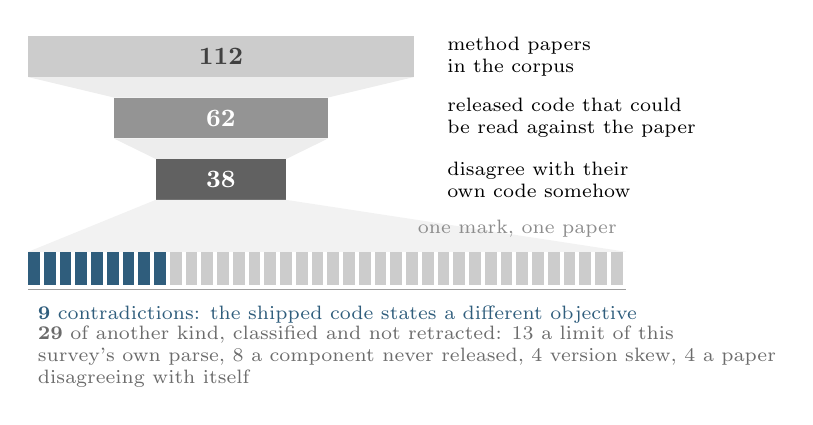
\begin{tikzpicture}[
  font=\footnotesize,
  bar/.style={draw=none,fill=black!62},
  barmid/.style={draw=none,fill=black!42},
  barlight/.style={draw=none,fill=black!20},
  baracc/.style={draw=none,fill=accent},
  seg/.style={draw=white,line width=0.5pt},
  lnk/.style={draw=black!38,line width=0.28pt},
  ghost/.style={draw=black!45,line width=0.3pt,dash pattern=on 1.2pt off 1.2pt},
  lbl/.style={font=\scriptsize},
  small/.style={font=\scriptsize\color{black!55}},
  num/.style={font=\scriptsize\color{black!55}},
]

\fill[barlight] (0.00,0.00) rectangle (4.90,-0.52);
\node[font=\small\bfseries\color{black!75}] at (2.45,-0.26) {112};
\node[lbl,anchor=west,align=left] at (5.20,-0.26) {method papers\\in the corpus};
\fill[black!7] (0.00,-0.52) -- (4.90,-0.52) -- (3.81,-0.78) -- (1.09,-0.78) -- cycle;
\fill[barmid] (1.09,-0.78) rectangle (3.81,-1.30);
\node[font=\small\bfseries\color{white}] at (2.45,-1.04) {62};
\node[lbl,anchor=west,align=left] at (5.20,-1.04) {released code that could\\be read against the paper};
\fill[black!7] (1.09,-1.30) -- (3.81,-1.30) -- (3.28,-1.56) -- (1.62,-1.56) -- cycle;
\fill[bar] (1.62,-1.56) rectangle (3.28,-2.08);
\node[font=\small\bfseries\color{white}] at (2.45,-1.82) {38};
\node[lbl,anchor=west,align=left] at (5.20,-1.82) {disagree with their\\own code somehow};
\fill[black!5] (1.62,-2.08) -- (3.28,-2.08) -- (7.60,-2.74) -- (0,-2.74) -- cycle;
\node[anchor=south east,font=\scriptsize\color{black!45}] at (7.60,-2.68) {one mark, one paper};
\fill[baracc] (0.00,-2.74) rectangle (0.15,-3.16);
\fill[baracc] (0.20,-2.74) rectangle (0.35,-3.16);
\fill[baracc] (0.40,-2.74) rectangle (0.55,-3.16);
\fill[baracc] (0.60,-2.74) rectangle (0.75,-3.16);
\fill[baracc] (0.80,-2.74) rectangle (0.95,-3.16);
\fill[baracc] (1.00,-2.74) rectangle (1.15,-3.16);
\fill[baracc] (1.20,-2.74) rectangle (1.35,-3.16);
\fill[baracc] (1.40,-2.74) rectangle (1.55,-3.16);
\fill[baracc] (1.60,-2.74) rectangle (1.75,-3.16);
\fill[barlight] (1.80,-2.74) rectangle (1.95,-3.16);
\fill[barlight] (2.00,-2.74) rectangle (2.15,-3.16);
\fill[barlight] (2.20,-2.74) rectangle (2.35,-3.16);
\fill[barlight] (2.40,-2.74) rectangle (2.55,-3.16);
\fill[barlight] (2.60,-2.74) rectangle (2.75,-3.16);
\fill[barlight] (2.80,-2.74) rectangle (2.95,-3.16);
\fill[barlight] (3.00,-2.74) rectangle (3.15,-3.16);
\fill[barlight] (3.20,-2.74) rectangle (3.35,-3.16);
\fill[barlight] (3.40,-2.74) rectangle (3.55,-3.16);
\fill[barlight] (3.60,-2.74) rectangle (3.75,-3.16);
\fill[barlight] (3.80,-2.74) rectangle (3.95,-3.16);
\fill[barlight] (4.00,-2.74) rectangle (4.15,-3.16);
\fill[barlight] (4.20,-2.74) rectangle (4.35,-3.16);
\fill[barlight] (4.40,-2.74) rectangle (4.55,-3.16);
\fill[barlight] (4.60,-2.74) rectangle (4.75,-3.16);
\fill[barlight] (4.80,-2.74) rectangle (4.95,-3.16);
\fill[barlight] (5.00,-2.74) rectangle (5.15,-3.16);
\fill[barlight] (5.20,-2.74) rectangle (5.35,-3.16);
\fill[barlight] (5.40,-2.74) rectangle (5.55,-3.16);
\fill[barlight] (5.60,-2.74) rectangle (5.75,-3.16);
\fill[barlight] (5.80,-2.74) rectangle (5.95,-3.16);
\fill[barlight] (6.00,-2.74) rectangle (6.15,-3.16);
\fill[barlight] (6.20,-2.74) rectangle (6.35,-3.16);
\fill[barlight] (6.40,-2.74) rectangle (6.55,-3.16);
\fill[barlight] (6.60,-2.74) rectangle (6.75,-3.16);
\fill[barlight] (6.80,-2.74) rectangle (6.95,-3.16);
\fill[barlight] (7.00,-2.74) rectangle (7.15,-3.16);
\fill[barlight] (7.20,-2.74) rectangle (7.35,-3.16);
\fill[barlight] (7.40,-2.74) rectangle (7.55,-3.16);
\draw[lnk] (0,-3.22) -- (7.60,-3.22);
\node[anchor=north west,align=left,font=\scriptsize\color{accent}] at (0,-3.30) {\textbf{9} contradictions: the shipped code states a different objective};
\node[anchor=north west,align=left,font=\scriptsize\color{black!58}] at (0,-3.56) {\textbf{29} of another kind, classified and not retracted: 13 a limit of this\\survey's own parse, 8 a component never released, 4 version skew, 4 a paper\\disagreeing with itself};
\end{tikzpicture}
}}{%
    \framebox[0.95\columnwidth]{\rule{0pt}{2.2cm}\textit{figs/fig\_codegap.tex pending}}}
  \caption{Papers disagree with their own released code, and the funnel ends at the \fnKept{} the survey stands behind as contradictions. Section~\ref{sec:train:code} classifies all \fnDisagree{} and names them.}
  \label{fig:codegap}
\end{figure}

Thirty-eight of the 112 method rows record a discrepancy between a paper and the code it released,
and all 38 released code, so they sit inside the 62 rows that released anything
(\figurename~\ref{fig:codegap}). They are not one kind of thing. Nine are contradictions, where
paper and code state different values or different terms. Thirteen are limits of this survey's own
parse, where the body or config that would settle the question was never recovered and the row
says so. Eight released code without the described component in it, four are version skew against
a later repository, and four are a paper disagreeing with itself. The fourth version skew is
\cite{groot_n16_2025}, which ships a main branch one generation later than the checkpoint its page
describes.

Nine is the number to quote, eight at high confidence and one, PenSpin \cite{penspin_2024}, held
at medium pending a direct read of the code. Nine of 62 is 15 percent, bounded on both sides: a
floor, because the census covers method rows only and RoboPianist \cite{robopianist_2023}, whose
row is a benchmark, sums five reward terms against the three its Table~2 documents; a ceiling,
because eight accusations an earlier draft of this section made were withdrawn, seven of them
under adversarial review and an eighth, OmniH2O \cite{omnih2o_2024}, once writing to its authors
sent someone back to the evidence, each with its reason recorded in the accused row beside the
charge. Among the 21 reorientation methods scored term by term, seven released a repository and
four of those disagree with their paper, the other three being a missing environment, a later
generation and a default-value question their own READMEs settle.

The most consequential case is \cite{physhoi_2023}. Its \texttt{compute\_humanoid\_reward}
hardcodes the body position-velocity error and both object rotation errors to zero, with the real
computation commented out beside them, and does so unconditionally rather than per dataset, while
its Table~4 lists non-zero weights of 0.1 and 0.01 for those rotation terms on GRAB. The reward
that produced the paper's numbers never tracked object orientation: a method presented as tracking
a 6-DoF reference was, in the code that ran, tracking the object in position only, with body
rotation and body rotation-velocity still live.

Zeroed terms recur, and are not the same failure. A term present and zeroed is worse than a term
missing, because it survives a reader's check of the file, but only when the paper claims it.
Weights drift as well: a penalty printed at one value in a table and shipped at another, an
equation's term absent from the released reward file, a term in the code that the table never
lists. And in 13 rows the repository does not settle the question at all, which is this survey's
limit and not an accusation. Appendix~\ref{app:rewards} prints all 38 row by row in
their five classes, each with the file, the value on both sides, and the review note where a charge
was narrowed or withdrawn.

A reward table is a claim about a training run and the code is a claim about a repository. Here
the two contradict each other in nine cases, in the other 29 the released artefacts do not settle
the question, and in exactly one, \cite{hora_2022}, the repository says so itself. Read the reward
function before the reward table, and treat a printed weight as a hypothesis about the code.

\textbf{The withdrawals, and what would close it.} This is a result about publishing practice in
robot learning rather than about dexterous manipulation in particular: the dexterous corpus is its
sample, not its subject. Nine is also a floor, since 46 method rows released nothing to check and
four more are unsettled. The first count was sixteen. An adversarial re-reading withdrew six of
them outright, ManipTrans, Eureka, Open-TeleVision, DexMachina, ArtiGrasp and GraspXL
\cite{maniptrans_2025,eureka_2023,open_television_2024,dexmachina_2025,artigrasp_2023,graspxl_2024}:
two refuted by the accused repository's own README, two resting on reward code never in the parse,
one charging the code with structure the paper prints, one against a paper with no reward function.
It narrowed a seventh, DexPBT \cite{dexpbt_2023}, where the domain-randomisation half of the charge
is withdrawn and the zeroed reward term stands, so its row is still a contradiction and its
withdrawal takes nothing off the count. That left ten, and ten held until the letters to the authors
were drafted. Drafting the letter to OmniH2O \cite{omnih2o_2024} meant reading its accusation once
more before it went out, and that second reading is what broke it. Four of its five reward-weight
comparisons match the paper's own table to the digit once a systematic $\times 1.25$ curriculum
factor is applied, and only the stumble weight differs, by a factor of about a million: a typo
signature in the paper's own table, not a policy trained on a different objective. The work's hands
are also driven open-loop from a VR pose, outside the policy and outside the reward, which made it a
poor fit for a dexterous-manipulation reward census whatever the weight said. The charge is
withdrawn and the row reclassified as an internal inconsistency, which is where the count above
already places it.

\textbf{The survey has now withdrawn eight accusations in total: seven of them under adversarial
review, and the eighth at the point of writing to the authors, because someone sat down to write the
letter and looked at the evidence again.} Each retraction and narrowing is recorded in its row
beside the charge: a survey that names people should carry its corrections beside its accusations,
in print and not only in the corpus. What would close the finding itself is a reward table generated
from the released config at a named commit, so that a reviewer diffs two artefacts instead of
reading two documents.


%% Section 6, Bimanual dexterous manipulation. Converted from paper/sections/06_bimanual.md.
\section{Bimanual dexterous manipulation}
\label{sec:bimanual}

% --- reproduced plates ------------------------------------------------------
% tex/figs/plates.tex defines one command per selected photograph. Load it here
% if nothing has loaded it already, so this section carries its own plates
% whether or not the preamble inputs the file. The \providecommand before each
% call makes a missing plate an empty command rather than an error. Every plate
% carries \pending: read tex/PERMISSIONS.md before this goes anywhere.
% ---------------------------------------------------------------------------
\makeatletter
\@ifundefined{plateGraspPenetration}{\IfFileExists{figs/plates.tex}{% The one reproduced plate.
% Rebuilt from its source PDF by tools/relayout_plates.py; see tex/figs/SELECTED.md for the crop
% box and tex/PERMISSIONS.md for the licence it is used under.
%
% A plate is kept only where a photograph or a render carries something a drawing cannot, and
% only where the paper has the right to print it without asking anyone. Everything else that was
% reproduced has been redrawn in the paper's own style (figs/fig_transmission, fig_collision,
% fig_tactiledepth, fig_contactlabel, fig_retarget) or dropped, because the prose already made the
% point or because no honest drawing could be made from what the corpus records. That took
% eighteen plates to one, eleven visual styles to four, and eleven open permissions to none.
%
% The survivor is single column and single panel. It is not a `figure*`: a borrowed plate has not
% earned the page width.
%
% One command for it. A section author places it by writing
%   \plateGraspPenetration
% at the point in the section where the float should be anchored, once: a plate called twice
% prints twice, on two pages, under two numbers.
%
% The plate credits its source inside its own caption with \src or \cite, and carries \licensed as
% well, because its source is CC BY 4.0 and the licence asks for an attribution line.

% ========================================================== Sec. VI, two hands

\newcommand{\plateGraspPenetration}{%
  \begin{figure}[t]
    \centering
    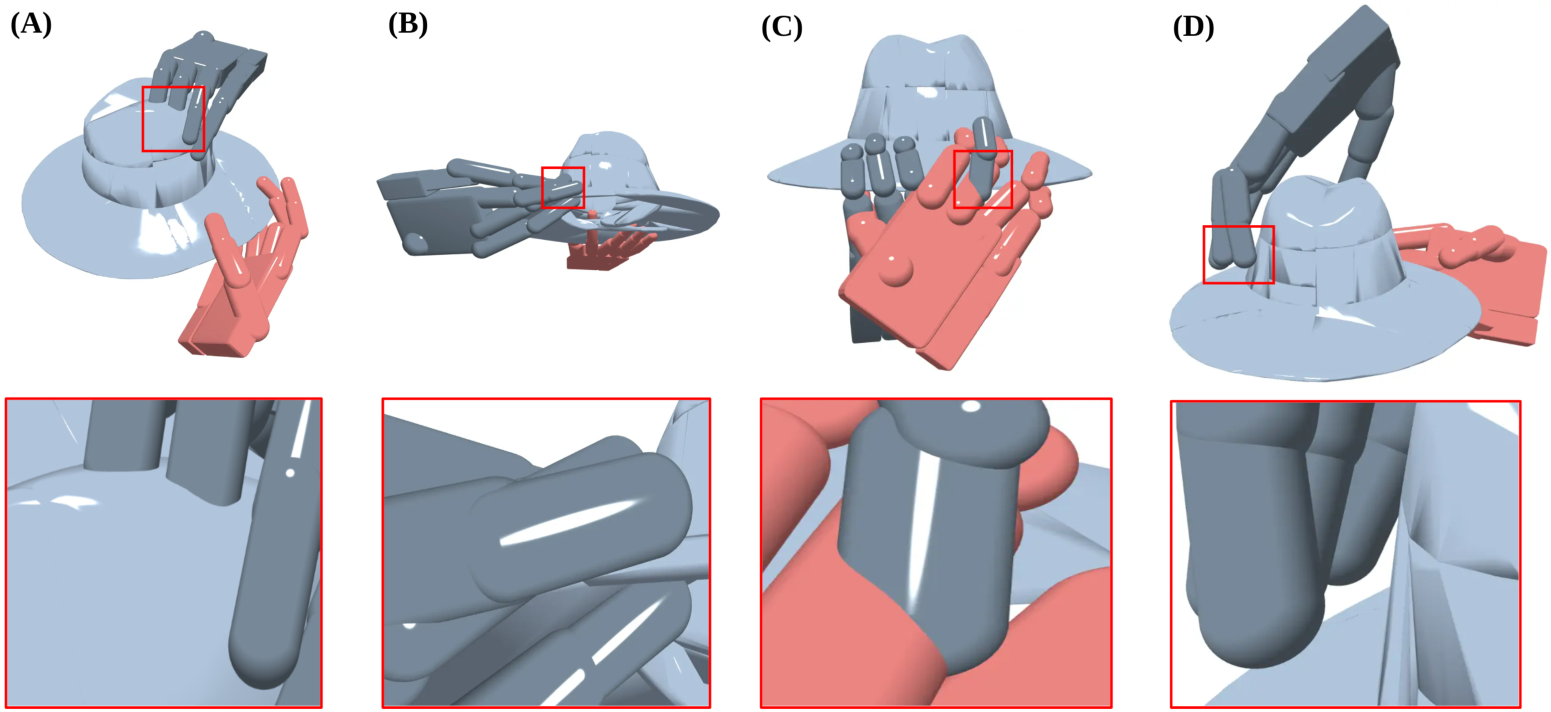
\includegraphics[width=0.86\columnwidth]{figs/selected/bimanual_grasp_penetration.png}
    \caption{Two failures of synthesised two-hand grasps, each enlarged at the
      contact: (A) a finger inside the object, (C) a finger inside the other hand.
      Both look plausible whole~\cite{bimangrasp_2024}.}
    \label{fig:bimanual-penetration}
    \licensed[panels (A) and (C) of Fig.~9]{Fig.~9 of Shao and Xiao, arXiv:2411.15903}{CC BY 4.0}{https://creativecommons.org/licenses/by/4.0/}
  \end{figure}}
}{}}{}
\makeatother

A warning first. Fifty-three corpus method rows carry the two-hand flag, and that flag says only
that the robot has two end effectors. Thirteen of the 53 put no dexterous hand on the robot at
all. ALOHA, RDT-1B, EgoMimic and H-RDT \cite{aloha_act_2023,rdt1b_2024,egomimic_2024,h_rdt_2025}
and UMI \cite{umi_2024} are parallel-jaw throughout; $\pi_0$, $\pi_{0.5}$ and $\pi^{*}_{0.6}$
\cite{pi0_2024,pi05_2025,pistar06_2025} and Diffusion Policy \cite{diffusion_policy_2023} name no
hand and run grippers on every embodiment; Gemini Robotics \cite{gemini_robotics_2025} and Gemini
Robotics 1.5 \cite{gemini_robotics_15_2025} report every bimanual number on grippers and show
five-fingered hands only qualitatively; and Helix \cite{helix_2025} and GR00T N1.6
\cite{groot_n16_2025} name no end effector anywhere on the page. Three more run a gripper on one
embodiment and a hand on another: ACE and 3D Diffusion Policy \cite{ace_teleop_2024,dp3_2024} and
Open-TeleVision \cite{open_television_2024}, whose Unitree H1 carries 6-DoF Inspire hands and
whose Fourier GR-1 carries a 1-DoF jaw.

\textbf{The denominator for this section is 28}: the method rows whose notes place a learned
closed-loop controller on two multi-fingered hands. It is the 53 less those 16; less two static
grasp-synthesis methods, BimanGrasp \cite{bimangrasp_2024} and BiDexGrasp \cite{bidexgrasp_2026};
less three systems with no learned policy, Castro et al. and DexTeleop-0
\cite{castro_sap_contact_2021,dexteleop0_2026} and Pang et al. \cite{pang_global_planning_2022};
and less four rows where no learned policy holds both hands: OmniH2O \cite{omnih2o_2024}, whose
fingers are mapped open-loop from the Vision Pro and sit outside its 19-DoF policy; OKAMI
\cite{okami_2024}, whose headline pipeline is open-loop retargeting with a learned policy only in
a side experiment; DexDeform \cite{dexdeform_2023}, a skill model refined by trajectory
optimisation rather than a closed-loop controller; and Omnigrasp \cite{omnigrasp_2024}, a
simulated human body with no bimanual task. Frau-Alfaro et al. \cite{dexterous_handover_2025}
never enter, because their row records one hand. Benchmarks and datasets are outside the 28 by
class, Bi-DexHands and Bench2Dex \cite{bidexhands_2022,bench2dex_2026} and RoboPianist
\cite{robopianist_2023} being benchmarks and RP1M \cite{rp1m_2024} and HumanoidGen
\cite{humanoidgen_2025} datasets; they are quoted here as evidence and never counted. Every paper
below runs two multi-fingered hands unless said otherwise.

\subsection{Why two hands is not twice one hand}
\label{subsec:two_not_twice}

When both hands hold the same object, the object closes a kinematic loop between them. Neither
hand can move without changing what the other must do. BiDexGrasp \cite{bidexgrasp_2026} reports
that the coupled objective ``often yields imbalanced solutions, where one hand dominates stability
while the other contributes marginally.'' ArtiGrasp \cite{artigrasp_2023} reports simulation speed
scaling ``roughly quadratically with the number of contacts,'' and trains each hand alone before
pairing them.

Role asymmetry is an assumption almost everyone makes silently. BiDexHD \cite{bidexhd_2024} states
it outright: ``we assume the robot to be right-handed by default, i.e., the left hand handles the
target object and the right hand handles the tool,'' and Lin et al. \cite{twisting_lids_2024} bake
the same split into their reward, putting reference contact keypoints on the bottle base for the
left fingertips and on the lid for the right. The bias is in the data first: TACO \cite{taco_2024}
recruited 14 right-handed subjects and measures the right hand moving consistently faster.

The arms collide, and the corpus handles this by construction rather than by control. RoboPianist
\cite{robopianist_2023} ships a forearm-forearm collision term that its own reward table never
lists. Two papers name arm collision as unsolved. DexMimicGen \cite{dexmimicgen_2024} ``does not
explicitly handle collisions,'' and DexMan \cite{dexman_2025} says its control parameterisation
``overlooks full arm posture,'' which it needs to avoid them.

The action space doubles and the observation grows faster. Bi-DexHands \cite{bidexhands_2022} uses
a 52-dimensional action for 18 of its 20 tasks against observations of 398 to 446 dimensions.
GR-Dexter \cite{gr_dexter_2025} emits an 88-dimensional chunk of arm joints, end-effector poses,
hand joints and fingertips. What the larger vector does not carry is any statement of who does
what. The usual answer is one scalar reward summed over both sides, and the cost is a compounding
failure rate. ManipTrans \cite{maniptrans_2025} scores success only if both hands succeed, and its
OakInk-V2 success rate falls from 58.1 percent on single-hand sequences to 39.5 percent on
bimanual ones.

\subsection{Coordination architectures}
\label{subsec:coordination}

\begin{figure*}[!t]
\centering
\IfFileExists{figs/fig_bimanual.tex}{% hand-drawn to match the style of tools/make_tikz_figures.py output
% Four coordination architectures for two dexterous hands. Greyscale plus the
% one accent; thin rules; square corners. Drawn at two-column width.
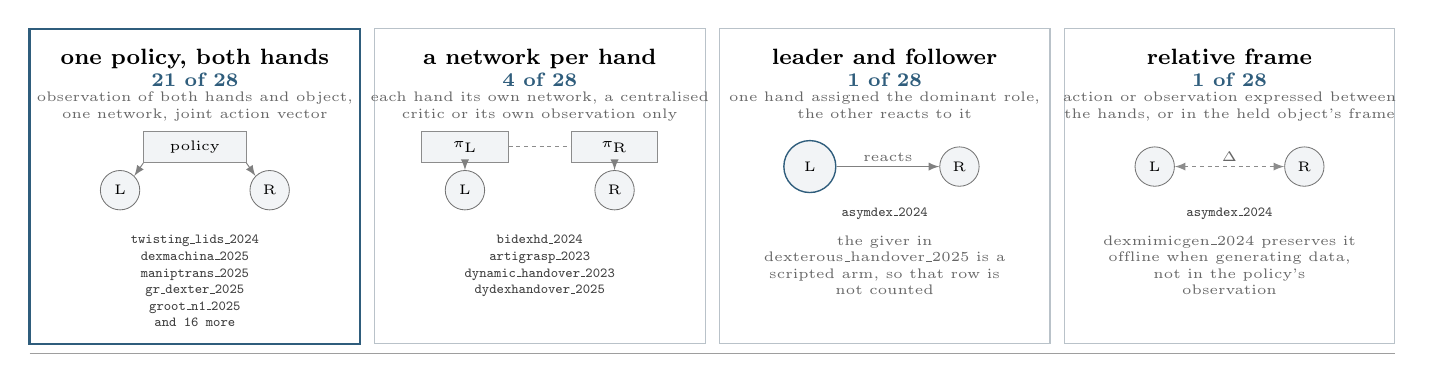
\begin{tikzpicture}[
  font=\footnotesize,
  panel/.style={draw=rule,line width=0.4pt,inner sep=0pt},
  panelacc/.style={draw=accent,line width=0.8pt,inner sep=0pt},
  box/.style={draw=black!45,fill=wash,line width=0.3pt,inner sep=0pt,align=center},
  hand/.style={draw=black!55,fill=wash,line width=0.3pt,circle,inner sep=0pt,minimum size=5.0mm,
               font=\tiny},
  handbig/.style={hand,draw=accent,line width=0.5pt,minimum size=6.6mm},
  lnk/.style={draw=black!50,line width=0.35pt,-latex},
  soft/.style={draw=black!45,line width=0.35pt,dash pattern=on 1.4pt off 1.4pt},
  hd/.style={font=\footnotesize\bfseries,align=center,anchor=north},
  cnt/.style={font=\scriptsize\bfseries\color{accent},anchor=north},
  dsc/.style={font=\tiny\color{black!60},align=center,anchor=north},
  ky/.style={font=\tiny\ttfamily\color{black!75},align=center,anchor=north},
]

% ---------------------------------------------------------------- panel 1 ----
\begin{scope}[shift={(0,0)}]
  \node[panelacc,minimum width=42mm,minimum height=40mm] at (2.1,2.00) {};
  \node[hd] at (2.1,3.86) {one policy, both hands};
  \node[cnt] at (2.1,3.56) {21 of 28};
  \node[dsc] at (2.1,3.32) {observation of both hands and object,\\one network, joint action vector};
  \node[box,minimum width=13mm,minimum height=4.0mm,font=\tiny] (p1) at (2.1,2.50) {policy};
  \node[hand] (l1) at (1.15,1.95) {L};
  \node[hand] (r1) at (3.05,1.95) {R};
  \draw[lnk] (p1.south west) -- (l1.north east);
  \draw[lnk] (p1.south east) -- (r1.north west);
  \node[ky] at (2.1,1.50) {twisting\_lids\_2024\\dexmachina\_2025\\maniptrans\_2025\\gr\_dexter\_2025\\groot\_n1\_2025\\and 16 more};
\end{scope}

% ---------------------------------------------------------------- panel 2 ----
\begin{scope}[shift={(4.38,0)}]
  \node[panel,minimum width=42mm,minimum height=40mm] at (2.1,2.00) {};
  \node[hd] at (2.1,3.86) {a network per hand};
  \node[cnt] at (2.1,3.56) {4 of 28};
  \node[dsc] at (2.1,3.32) {each hand its own network, a centralised\\critic or its own observation only};
  \node[box,minimum width=11mm,minimum height=4.0mm,font=\tiny] (a2) at (1.15,2.50) {$\pi_{\mathrm{L}}$};
  \node[box,minimum width=11mm,minimum height=4.0mm,font=\tiny] (b2) at (3.05,2.50) {$\pi_{\mathrm{R}}$};
  \node[hand] (l2) at (1.15,1.95) {L};
  \node[hand] (r2) at (3.05,1.95) {R};
  \draw[soft] (a2.east) -- (b2.west);
  \draw[lnk] (a2.south) -- (l2.north);
  \draw[lnk] (b2.south) -- (r2.north);
  \node[ky] at (2.1,1.50) {bidexhd\_2024\\artigrasp\_2023\\dynamic\_handover\_2023\\dydexhandover\_2025};
\end{scope}

% ---------------------------------------------------------------- panel 3 ----
\begin{scope}[shift={(8.76,0)}]
  \node[panel,minimum width=42mm,minimum height=40mm] at (2.1,2.00) {};
  \node[hd] at (2.1,3.86) {leader and follower};
  \node[cnt] at (2.1,3.56) {1 of 28};
  \node[dsc] at (2.1,3.32) {one hand assigned the dominant role,\\the other reacts to it};
  \node[handbig] (l3) at (1.15,2.25) {L};
  \node[hand] (r3) at (3.05,2.25) {R};
  \draw[lnk] (l3.east) -- node[above,font=\tiny\color{black!60},inner sep=1.5pt] {reacts} (r3.west);
  \node[ky] at (2.1,1.85) {asymdex\_2024};
  \node[dsc] at (2.1,1.50) {the giver in\\dexterous\_handover\_2025 is a\\scripted arm, so that row is\\not counted};
\end{scope}

% ---------------------------------------------------------------- panel 4 ----
\begin{scope}[shift={(13.14,0)}]
  \node[panel,minimum width=42mm,minimum height=40mm] at (2.1,2.00) {};
  \node[hd] at (2.1,3.86) {relative frame};
  \node[cnt] at (2.1,3.56) {1 of 28};
  \node[dsc] at (2.1,3.32) {action or observation expressed between\\the hands, or in the held object's frame};
  \node[hand] (l4) at (1.15,2.25) {L};
  \node[hand] (r4) at (3.05,2.25) {R};
  \draw[soft,latex-latex] (l4.east) -- node[above,font=\tiny\color{black!60},inner sep=1.5pt] {$\Delta$} (r4.west);
  \node[ky] at (2.1,1.85) {asymdex\_2024};
  \node[dsc] at (2.1,1.50) {dexmimicgen\_2024 preserves it\\offline when generating data,\\not in the policy's\\observation};
\end{scope}

\draw[draw=black!38,line width=0.28pt] (0,-0.12) -- (17.34,-0.12);
\end{tikzpicture}
}{%
  \framebox[0.7\textwidth]{\rule{0pt}{2.2cm}\textit{figs/fig\_bimanual.tex pending}}}
\caption{Four ways to control two dexterous hands. Counts are over the 28 corpus rows that put a
learned closed-loop controller on two multi-fingered hands, each read from its note. The four
architectures do not partition the 28: AsymDex \cite{asymdex_2024} is counted in both of the last
two panels, being the only corpus paper that puts either mechanism inside a policy, and
Bunny-VisionPro \cite{bunny_visionpro_2024} and DexImit \cite{deximit_2026} are unassigned because
their notes describe
the rig and the data pipeline rather than the policy's decomposition. The field is concentrated in
the first panel; the two on the right are where the structure of the problem is actually used.}
\label{fig:bimanual}
\end{figure*}

\figurename~\ref{fig:bimanual} sets the four architectures side by side. Every row of the 28 is
assigned to exactly one of them, read from its note.

Twenty-one of the 28 put one policy over both hands, which is three quarters of the set: the
trackers and tracking-adjacent methods
\cite{dexmachina_2025,dexman_2025,maniptrans_2025,objdex_2024} and \cite{humanplus_2024}; the
reinforcement-learning tasks \cite{dexpbt_2023,twisting_lids_2024,eureka_2023,pianomime_2024} and
\cite{humanoid_sim2real_recipe_2025}; the demonstration pipelines
\cite{bidex_teleop_2024,dexcap_2024,dexwild_2025,dexmimicgen_2024,hato_visuotactile_2024} and
\cite{humanoid_policy_human_policy_2025}; and the generalist policies
\cite{gr_dexter_2025,groot_n1_2025,dexora_2026,metis_2025} and \cite{egoscale_2026}. In every one
of them a single network takes a concatenated two-hand observation and emits a two-hand action.
Two rows do not say which they are, Bunny-VisionPro \cite{bunny_visionpro_2024} and DexImit
\cite{deximit_2026}, whose notes describe the rig and the data pipeline but never the policy's own
decomposition. The concentration is not the outcome of a comparison that was won.

Four of the 28 give each hand its own network, and the two papers that compare the choice
disagree. Bi-DexHands \cite{bidexhands_2022}, a benchmark row and so outside the 28, ships the
MARL baselines and finds PPO over the full observation beats HAPPO and MAPPO ``in most cases,''
with the gap narrowing on tasks that need both hands, because PPO ``can use all observations''
where MARL sees only part. BiDexHD \cite{bidexhd_2024} concludes the opposite. Its independent PPO
teachers score 74.59 percent stage-two tracking rate on trained tasks against 53.88 for a
centralised policy over both observations. Both are simulation only, on different tasks and hands,
so neither settles it. ArtiGrasp \cite{artigrasp_2023} trains one PPO policy per hand, and Dynamic
Handover \cite{dynamic_handover_2023} and DyDexHandover \cite{dydexhandover_2025} use MAPPO with
one agent per arm-hand system.

One of the 28 assigns explicit leader and follower roles, and the same one is the only policy
expressed in a relative frame. AsymDex \cite{asymdex_2024} is that paper, and the only corpus
paper that puts either mechanism inside a policy. It gives the dominant hand full finger and wrist
control, restricts the facilitating hand to a 6-DoF base pose, and writes the dominant hand and
the object in a frame attached to the object the facilitating hand holds. That cuts the
observation from 176 dimensions to 88 and the action from 52 to 26. It ablates the two mechanisms
separately, which no other corpus paper does. On Block in cup the full method scores 0.7701 over
five seeds, against 0.1086 for relative frames without asymmetry and 0.0164 for asymmetry without
them. Twist Lid transfers zero-shot at 18 of 20 real trials. The real rig pairs a 16-DoF Allegro
with a 6-DoF Ability Hand because only one Allegro was available, so the roles are confounded with
the hardware. Two other rows use a relative quantity without giving either hand a role: DexWild
\cite{dexwild_2025} appends the inter-hand pose to its observation, and DexMimicGen
\cite{dexmimicgen_2024} applies one shared SE(3) transform to both arms' source segments when
generating data, which is the mechanism offline rather than in a policy.

\subsection{Benchmarks and datasets for two hands}
\label{subsec:bimanual_benchmarks}

Two purpose-built bimanual dexterous suites exist in the corpus, four years apart.

Bi-DexHands \cite{bidexhands_2022} is 20 tasks on two Shadow Hands in Isaac Gym, ordered by the
infant age at which humans acquire the skill, at 2048 environments and a reported 30,000-plus FPS.
Its measurement discipline is weaker than its coverage. It reports reward and normalised score,
never a success rate. Its only success flag in code tests the object-to-goal distance against 3
cm, which ignores orientation and exists only in the four catching tasks. Any success rate later
work attributes to Bi-DexHands comes from that flag or its own definition.

Bench2Dex \cite{bench2dex_2026} is the more instrumented of the two. It runs 26 long-horizon tasks
in Isaac Lab across 12 arm-and-hand embodiments, with roughly 1.3K teleoperated demonstrations in
eight modalities, including a ray-cast tactile image that maps all 12 hand geometries into one
representation. Success needs the terminal predicate held for 0.5 s. Matched, GR00T N1.5 leads at
631 of 1300 rollouts, 48.5 percent, against ACT at 29.5, $\pi_{0.5}$ at 27.3 and Diffusion Policy
at 12.9. Under combined perturbation those first two compress to 19.8 and 19.7. Tasks are not
crossed with embodiments, so no contrast isolates the hand, and the authors state the hand and
tactile models are not calibrated against matching physical hardware.

Ten corpus rows are bimanual datasets, and five are two-hand interaction capture. ARCTIC
\cite{arctic_2022} gives 339 mocap sequences of 11 one-DoF articulated objects held in both hands,
and deliberately labels over-shooting vertices as in contact, so its ground truth records
interpenetration as contact. TACO \cite{taco_2024} gives 2.5K bimanual tool-use sequences fitted
markerlessly under an attraction loss and a penetration loss the paper says trade against each
other. OakInk-V2 \cite{oakink2_2024} is the only corpus dataset publishing a penetration number
for its own annotations, a mean depth of 0.25 cm over its 627 long-horizon sequences. HOT3D
\cite{hot3d_2024} gives 833 egocentric minutes with mocap-grade poses for both hands and up to six
objects, and GigaHands \cite{gigahands_2024} gives 2,034 markerless minutes from 56 subjects,
neither with a penetration metric. These five feed the tracking work here: DexMachina
\cite{dexmachina_2025} and ArtiGrasp \cite{artigrasp_2023} from ARCTIC, BiDexHD
\cite{bidexhd_2024} from TACO, ManipTrans \cite{maniptrans_2025} from OakInk-V2 and DexMan
\cite{dexman_2025} from both.

% From source video to fitted meshes and a contact field.
\providecommand{\plateArcticDataset}{}\plateArcticDataset

\subsection{Methods on the same axes}
\label{subsec:bimanual_axes}

The method tabulation carries the bimanual papers on the same columns as every other method here,
and three of those columns are worth reading together.

Real trials. AsymDex \cite{asymdex_2024} reports 20 per task, HATO \cite{hato_visuotactile_2024}
10 per condition, DexMimicGen \cite{dexmimicgen_2024} 20 on a Fourier GR1 and BiDexGrasp
\cite{bidexgrasp_2026} 260 across 30 objects. ManipTrans \cite{maniptrans_2025} reaches real
Inspire hands by open-loop replay with no trial count and no success rate. Seven of the 28 have no
real robot at all:
\cite{artigrasp_2023,bidexhd_2024,dexmachina_2025,dexman_2025,dexpbt_2023,dydexhandover_2025} and
\cite{pianomime_2024}. The two piano rows outside the denominator, RoboPianist
\cite{robopianist_2023} and RP1M \cite{rp1m_2024}, are simulation-only as well.

% The four commonest failures of two-hand grasp synthesis, at the scale of the contact.
\providecommand{\plateGraspPenetration}{}\plateGraspPenetration

Penetration. Most bimanual rows read ``not addressed.'' BimanGrasp \cite{bimangrasp_2024} gates on
it, failing any grasp whose total penetration across hand-object, self and inter-hand exceeds 1.5
mm, and reports that ``penetration remains the primary cause of grasp failure.'' BiDexGrasp
\cite{bidexgrasp_2026} reports it as a number, 0.15 to 0.20 cm maximum depth for its own grasps.
DexImit \cite{deximit_2026} carries a named hand-hand penetration term in its grasp-synthesis
objective. DexMachina \cite{dexmachina_2025} resolves it once, replaying retargeted joints against
a fixed object ``to eliminate object penetrations'' and measuring nothing during rollout.
ArtiGrasp \cite{artigrasp_2023} declines the metric outright, because its baselines ``include a
physics simulation which exhibits no interpenetration.''

Comparability. BimanGrasp \cite{bimangrasp_2024} reports 54.03 percent success in Isaac Gym at
friction 3. BiDexGrasp \cite{bidexgrasp_2026} re-runs the same grasps in MuJoCo at friction 0.6
and gets 26.80 percent, at 1.52 cm penetration depth. Neither number transfers, and
Section~\ref{sec:train:track}'s re-implementation result is the same lesson on the training side.

\subsection{Handover and in-hand transfer}
\label{subsec:handover}
% Two arms, two hands, and no contact between them but the object's flight.
\providecommand{\plateHandoverAllegro}{}\plateHandoverAllegro

Handover is the one bimanual task where the hands are unambiguously asymmetric, because one gives
and one receives. All three corpus handover papers use a single shared reward across giver and
receiver. None defines separate objectives for the two roles.

Dynamic Handover \cite{dynamic_handover_2023} states one formula, $r = r_{\mathrm{dis}} +
r_{\mathrm{linvel}} + r_{\mathrm{torque}}$, and never says whether thrower and catcher receive
different decompositions of it. DyDexHandover \cite{dydexhandover_2025} is explicit that they do
not: ``Both hands share aligned objectives, forming a fully cooperative relationship,'' with one
weighted sum feeding both agents. Only the thrower gets an extra KL regulariser toward a policy
pretrained on human throws, which constrains style and not role.

The third case is weaker still. In \cite{dexterous_handover_2025} only the receiver is learned.
The giver is a UR5e with an Allegro hand that ``holds the object without moving during the whole
episode.'' There is one agent, one reward and no second policy, its corpus row accordingly records
one hand, and it is one of the rows the 28 excludes. The 94 percent often attached to this paper
needs its conditions. It is Total Success, which counts ``Indetermination'' cases where the
simulator failed to resolve collisions and the object clipped through the giver's hand, on the
short prism, in simulation, over 100 episodes, with no real robot in the paper.

Nothing in the handover literature measures contact quality. Contact appears only as a positive
signal, a boolean per-phalange touch in \cite{dexterous_handover_2025} and a boolean contact
reward in \cite{dydexhandover_2025}. The two systems that do handover well sidestep the problem.
HATO \cite{hato_visuotactile_2024} reaches 10 of 10 on a real slippery handover by imitating
teleoperation with fingertip touch sensing and no physics model. Lin et al.
\cite{humanoid_sim2real_recipe_2025} stage their reward with a discrete variable switching which
hand's fingertips are scored, and still calls handover its hardest task at 52.5 percent real
success.

\subsection{What transfers from single-hand work}
\label{subsec:bimanual_transfer}

The training recipe transfers intact. PPO with thousands of parallel environments, an asymmetric
critic on privileged state, domain randomisation and distillation into a vision policy is the same
in \cite{twisting_lids_2024} and \cite{humanoid_sim2real_recipe_2025} as in
Section~\ref{sec:train:rl}. Reward forms transfer literally, and the contact-goal reward
$r_{\mathrm{contact}} = \sum 1/(1+\alpha d)$ appears in both.

Multi-task learning does not transfer, and the bimanual benchmarks show it clearest. Bi-DexHands
\cite{bidexhands_2022} finds multi-task PPO and ProMP fail on MT4, MT20, ML4 and ML20. RoboPianist
\cite{robopianist_2023} finds F1 on the shared training song drops ``from roughly 0.7 F1 for 1
song to almost 0 F1 for 16 songs,'' with no positive transfer ``regardless of the size of the
pre-training tasks.''

Single-hand evaluation does not transfer either. Success criteria compound, because ManipTrans
\cite{maniptrans_2025} fails a trajectory ``if either hand fails to meet these conditions.'' And
object-centric metrics cannot say which hand caused the failure. BiDexHD \cite{bidexhd_2024}
scores the steps where both objects track their references, and DexMachina \cite{dexmachina_2025}
averages ADD across object parts before an AUC. Both say whether the task worked and nothing about
which hand lost it.

One failure mode has no single-hand counterpart. Two hands can penetrate each other, and the
corpus almost never looks. Three papers carry an inter-hand penetration term, and all three are
static grasp synthesis: \cite{bimangrasp_2024,bidexgrasp_2026} and \cite{deximit_2026}. Not one
learned bimanual controller in the corpus measures or penalises hand-hand penetration during a
rollout. PianoMime \cite{pianomime_2024} ships a flag that turns inter-hand collision off in the
physics.
%% Section 7, Evaluation. Converted from paper/sections/07_evaluation.md.
\section{Evaluation, and a protocol for comparison}
\label{sec:evaluation}

% No reproduced plate in this section: the photograph of the caged motion-capture
% rig that used to stand here illustrated a cost the paragraph below states in
% rollouts and hours, which is the form the reader can use.
% ---------------------------------------------------------------------------
\makeatletter
\@ifundefined{fnLoaded}{\IfFileExists{figs/finding_numbers.tex}{% generated by tools/make_finding_figures.py; do not edit
% Every count the finding figures and their captions print, recomputed from corpus/rows.
\providecommand{\fnLoaded}{}
\providecommand{\fnRows}{112}
\providecommand{\fnCode}{62}
\providecommand{\fnDisagree}{38}
\providecommand{\fnKept}{9}
\providecommand{\fnOtherClass}{29}
\providecommand{\fnParse}{13}
\providecommand{\fnAbsent}{8}
\providecommand{\fnSkew}{4}
\providecommand{\fnInternal}{4}
\providecommand{\fnPenSettled}{96}
\providecommand{\fnPenHandled}{11}
\providecommand{\fnPenClosed}{4}
\providecommand{\fnPenOther}{7}
\providecommand{\fnPenRollout}{0}
\providecommand{\fnTrials}{39}
\providecommand{\fnTrialsMedian}{15}
\providecommand{\fnTrialsMode}{10}
\providecommand{\fnTrialsModeN}{16}
\providecommand{\fnTotals}{24}
\providecommand{\fnTotalsMin}{12}
\providecommand{\fnTotalsMax}{750}
\providecommand{\fnUnclear}{7}
}{}}{}
\makeatother

\subsection{Reporting practice}
\label{subsec:reporting}

\begin{figure}[!t]
\centering
\IfFileExists{figs/fig_reporting.tex}{\resizebox{\columnwidth}{!}{% generated by tools/make_tikz_figures.py; do not edit
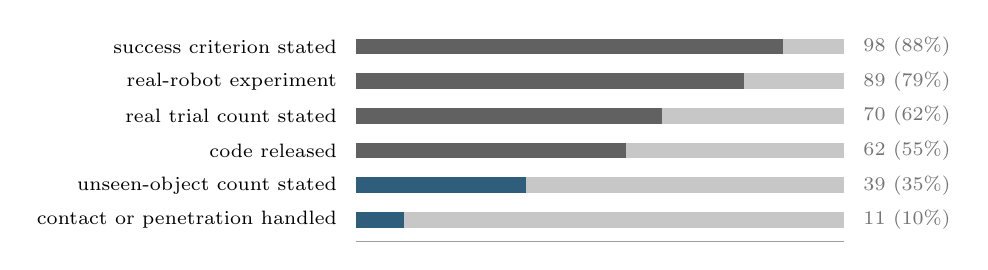
\begin{tikzpicture}[
  font=\footnotesize,
  bar/.style={draw=none,fill=black!62},
  barlight/.style={draw=none,fill=black!22},
  baracc/.style={draw=none,fill=accent},
  box/.style={draw=black!45,line width=0.3pt,inner sep=3pt,align=left},
  ghost/.style={draw=black!35,line width=0.3pt,dash pattern=on 1.4pt off 1.4pt,inner sep=3pt,align=left},
  lnk/.style={draw=black!38,line width=0.28pt},
  lbl/.style={font=\scriptsize},
  num/.style={font=\scriptsize\color{black!55}},
]

\node[lbl,anchor=east] at (0,-0.00) {success criterion stated};
\fill[barlight] (0.12,-0.10) rectangle (6.32,0.10);
\fill[bar] (0.12,-0.10) rectangle (5.54,0.10);
\node[num,anchor=west] at (6.44,-0.00) {98 (88\%)};
\node[lbl,anchor=east] at (0,-0.44) {real-robot experiment};
\fill[barlight] (0.12,-0.54) rectangle (6.32,-0.34);
\fill[bar] (0.12,-0.54) rectangle (5.05,-0.34);
\node[num,anchor=west] at (6.44,-0.44) {89 (79\%)};
\node[lbl,anchor=east] at (0,-0.88) {real trial count stated};
\fill[barlight] (0.12,-0.98) rectangle (6.32,-0.78);
\fill[bar] (0.12,-0.98) rectangle (4.00,-0.78);
\node[num,anchor=west] at (6.44,-0.88) {70 (62\%)};
\node[lbl,anchor=east] at (0,-1.32) {code released};
\fill[barlight] (0.12,-1.42) rectangle (6.32,-1.22);
\fill[bar] (0.12,-1.42) rectangle (3.55,-1.22);
\node[num,anchor=west] at (6.44,-1.32) {62 (55\%)};
\node[lbl,anchor=east] at (0,-1.76) {unseen-object count stated};
\fill[barlight] (0.12,-1.86) rectangle (6.32,-1.66);
\fill[baracc] (0.12,-1.86) rectangle (2.28,-1.66);
\node[num,anchor=west] at (6.44,-1.76) {39 (35\%)};
\node[lbl,anchor=east] at (0,-2.20) {contact or penetration handled};
\fill[barlight] (0.12,-2.30) rectangle (6.32,-2.10);
\fill[baracc] (0.12,-2.30) rectangle (0.73,-2.10);
\node[num,anchor=west] at (6.44,-2.20) {11 (10\%)};
\draw[lnk] (0.12,-2.48) -- (6.32,-2.48);
\end{tikzpicture}}}{%
  \framebox[0.95\columnwidth]{\rule{0pt}{2.2cm}\textit{figs/fig\_reporting.tex pending}}}
\caption{What gets reported, and what does not: six shares of the 112 corpus method rows, each bar
drawn against the denominator the text gives, with the two rarest reporting practices marked in
colour.}
\label{fig:reporting}
\end{figure}

Of the 112 method rows in the corpus, 89 report a real-robot experiment, 22 do not and one row is
unsettled, which is 80 percent of the 111 the note settled. Among those 89, 70 state how many real
trials produced the headline number, 79 percent of them. The 89 is the denominator that belongs to
this statistic: the 22 rows with no real robot cannot state a real trial count, and counting them
as silent turns a definitional impossibility into a reporting failure. Thirty-nine rows state a
count of unseen test objects, 35 percent. Ninety-eight state how a rollout is scored, 88 percent.
Sixty-two released code and 46 did not, with four rows unsettled, 57 percent of the 108 the note
settled. \figurename~\ref{fig:reporting} draws these six shares, each against the denominator that
belongs to it. Every bar is a lower bound, for the reason the next paragraph sets out. Two of the
six are marked, because they are the pair a reader needs in order to compare any two methods:
without a count of unseen objects a success rate has no generalisation denominator, and without
contact or penetration handling it says nothing about whether the hand passed through the object.
They are also the two the field reports least.

\textbf{These are counts of what this survey captured, not of what papers reported, and every one
is a floor.} A structured row holds a scalar. A paper that reports ten trials on each of nine
tasks, or a scoring rubric instead of a threshold, or a count spread over four tables, has nothing
the extraction can reduce to one integer, so it produces a null, and a null is then
indistinguishable from a paper that said nothing. The bias runs one way: every miss converts a
reporting paper into a silent one, and the survey's argument is that the field reports badly, so
the artefact flatters the argument. Section~\ref{sec:train:code} makes the same disclosure about
the paper/code count, subtracting the 13 disagreements that are limitations of this survey's own
parsing before declaring which number to quote, and the coverage statistics above need it more.

The nulls behind those six shares were therefore audited by hand against the notes they came from,
and every number above is post-audit. Appendix~\ref{app:method} gives what that audit recovered and
what it could not: the counts moved by tens of rows, 19 trial counts and 4 criteria remain
genuinely unsettled, and every bar in \figurename~\ref{fig:reporting} is still a lower bound.

The remaining gap is the one that matters. Nineteen of the 89 papers with a real robot never say
how many times they ran it. A percentage with no denominator cannot be given an interval, so it
cannot be compared with anything.

Where the denominator is stated it is small, and it is not one quantity. Some stored counts are
per-cell, meaning ten trials on each task, or twenty per condition, or five per object. Others are
grand totals over every cell. The rows now record which of the two each value is, and the two
distributions are quoted separately. The 39 per-cell counts run from 5 to 100 with a median of 15
and quartiles at 10 and 20. The modal cell is 10 trials, in 16 rows, then 20, in 12. The 24 grand
totals run from 12 to 750 with a median of 110. Pooling the two gives a median of 20 and a range
of 5 to 1287, and that pooled figure is the one an earlier draft of this section quoted. It
describes nothing, because Hora \cite{hora_2022}'s 240 and Visual Dexterity
\cite{visual_dexterity_2022}'s 20 are experiments of comparable size recorded on different bases.
Seven further counts could not be assigned a basis at all. \figurename~\ref{fig:trials} is the
per-cell distribution.

% ---------------------------------------------------------------------------
% The per-cell real-trial counts. The grand totals are a different quantity and
% are not pooled into it. Written by tools/make_finding_figures.py.
% ---------------------------------------------------------------------------
\begin{figure}[!t]
  \centering
  \IfFileExists{figs/fig_trials.tex}{\resizebox{\columnwidth}{!}{% generated by tools/make_finding_figures.py; do not edit
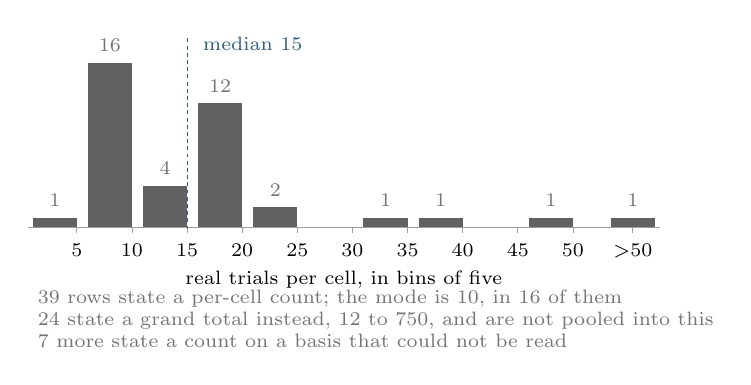
\begin{tikzpicture}[
  font=\footnotesize,
  bar/.style={draw=none,fill=black!62},
  barmid/.style={draw=none,fill=black!42},
  barlight/.style={draw=none,fill=black!20},
  baracc/.style={draw=none,fill=accent},
  seg/.style={draw=white,line width=0.5pt},
  lnk/.style={draw=black!38,line width=0.28pt},
  ghost/.style={draw=black!45,line width=0.3pt,dash pattern=on 1.2pt off 1.2pt},
  lbl/.style={font=\scriptsize},
  small/.style={font=\scriptsize\color{black!55}},
  num/.style={font=\scriptsize\color{black!55}},
]

\fill[bar] (0.00,0) rectangle (0.56,0.13);
\node[num,anchor=south] at (0.28,0.15) {1};
\draw[lnk] (0.56,0) -- (0.56,-0.06);
\node[lbl,anchor=north] at (0.56,-0.08) {5};
\fill[bar] (0.70,0) rectangle (1.26,2.10);
\node[num,anchor=south] at (0.98,2.12) {16};
\draw[lnk] (1.26,0) -- (1.26,-0.06);
\node[lbl,anchor=north] at (1.26,-0.08) {10};
\fill[bar] (1.40,0) rectangle (1.96,0.53);
\node[num,anchor=south] at (1.68,0.55) {4};
\draw[lnk] (1.96,0) -- (1.96,-0.06);
\node[lbl,anchor=north] at (1.96,-0.08) {15};
\fill[bar] (2.10,0) rectangle (2.66,1.58);
\node[num,anchor=south] at (2.38,1.60) {12};
\draw[lnk] (2.66,0) -- (2.66,-0.06);
\node[lbl,anchor=north] at (2.66,-0.08) {20};
\fill[bar] (2.80,0) rectangle (3.36,0.26);
\node[num,anchor=south] at (3.08,0.28) {2};
\draw[lnk] (3.36,0) -- (3.36,-0.06);
\node[lbl,anchor=north] at (3.36,-0.08) {25};
\draw[lnk] (4.06,0) -- (4.06,-0.06);
\node[lbl,anchor=north] at (4.06,-0.08) {30};
\fill[bar] (4.20,0) rectangle (4.76,0.13);
\node[num,anchor=south] at (4.48,0.15) {1};
\draw[lnk] (4.76,0) -- (4.76,-0.06);
\node[lbl,anchor=north] at (4.76,-0.08) {35};
\fill[bar] (4.90,0) rectangle (5.46,0.13);
\node[num,anchor=south] at (5.18,0.15) {1};
\draw[lnk] (5.46,0) -- (5.46,-0.06);
\node[lbl,anchor=north] at (5.46,-0.08) {40};
\draw[lnk] (6.16,0) -- (6.16,-0.06);
\node[lbl,anchor=north] at (6.16,-0.08) {45};
\fill[bar] (6.30,0) rectangle (6.86,0.13);
\node[num,anchor=south] at (6.58,0.15) {1};
\draw[lnk] (6.86,0) -- (6.86,-0.06);
\node[lbl,anchor=north] at (6.86,-0.08) {50};
\fill[bar] (7.34,0) rectangle (7.90,0.13);
\node[num,anchor=south] at (7.62,0.15) {1};
\draw[lnk] (7.62,0) -- (7.62,-0.06);
\node[lbl,anchor=north] at (7.62,-0.08) {$>$50};
\draw[lnk] (-0.06,0) -- (7.96,0);
\node[lbl,anchor=north] at (3.95,-0.42) {real trials per cell, in bins of five};
\draw[draw=accent,line width=0.4pt,dash pattern=on 1.4pt off 1.2pt] (1.96,-0.02) -- (1.96,2.44);
\node[anchor=west,font=\scriptsize\color{accent}] at (2.04,2.34) {median 15};
\node[small,anchor=north west,align=left] at (-0.06,-0.66) {39 rows state a per-cell count; the mode is 10, in 16 of them\\24 state a grand total instead, 12 to 750, and are not pooled into this\\7 more state a count on a basis that could not be read};
\end{tikzpicture}
}}{%
    \framebox[0.95\columnwidth]{\rule{0pt}{2.2cm}\textit{figs/fig\_trials.tex pending}}}
  \caption{Where a denominator is stated it is small: the \fnTrials{} per-cell real-trial counts,
  binned by fives, median \fnTrialsMedian{} marked. The \fnTotals{} grand totals are a separate
  quantity, counted beneath the axis rather than pooled in.}
  \label{fig:trials}
\end{figure}

The per-cell count is the one a Wilson interval attaches to. For $s$ successes in $n$ trials, with
$\hat{p} = s/n$ and $z = z_{1-\alpha/2} = 1.96$ at the 95 percent level, the bounds of that
interval are
\begin{equation}
\frac{2n\hat{p} + z^{2} \;\pm\; z\sqrt{4n\hat{p}\,(1-\hat{p}) + z^{2}}}{2\,(n + z^{2})},
\label{eq:wilson}
\end{equation}
which, unlike the normal approximation, stays inside $[0,1]$ and does not collapse to zero width at
$\hat{p} = 0$ or $\hat{p} = 1$. At 20 trials a reported 60 percent carries a 95 percent Wilson
interval of 39 to 78 percent, and a reported 80 percent an interval of 58 to 92 percent.
Overlapping intervals are not a test, so the point is made with one: 12 of 20 against 16 of 20 is
$z = 1.38$, $p = 0.17$, and the difference is not established. Two methods separated by 20 points
at 20 trials, the larger of the two modal cell sizes, are not separated at all.

The share of papers stating a count has risen, from 39 of the 65 rows before 2025, 60 percent, to
31 of the 47 rows from 2025 and 2026, 66 percent. The counts themselves have not. The median
stated count is 20 in 2024, 22.5 in 2025 and 20 in 2026. Before 2024 the per-year medians rest on
one to seven observations and should not be read as a trend.

The denominators also sit on different hardware. The 103 method rows that name their own hand give
78 distinct hand strings between them, and this survey applies no normalisation to those strings,
so 78 is a count of strings and not of hand designs. Matching on the string, Allegro appears in
35, Shadow in 21, Inspire in 19 and LEAP in 12. A success rate on a 16-degree-of-freedom Allegro
and a success rate on a 6-actuator Inspire hand are not measurements of the same thing.

Nor are the criteria. DexVerse
\cite{dexverse_2026} counts PickCube a success when the cube is ``lifted at least 0.20 m above its
resetting height''. Bench2Dex \cite{bench2dex_2026} requires its terminal predicate to hold for a
continuous dwell time of 0.5 s, to reject transient contacts. The Colosseum \cite{colosseum_2024}
counts an episode successful ``if the model completes the task fully''. DexTrack
\cite{dextrack_2025} reports every success rate as a pair under two threshold sets, which on GRAB
gives 46.70 and 65.48 percent for the same rollouts. Of the 14 rows that still state no criterion,
ten have no success predicate at all. They report radians rotated or time-to-fall and never define
a success, which is a fact about the paper rather than a gap in this survey. And four are
unsettled by the note. Of the 19 criteria the audit recovered, all but one are a rubric, a staged
partial credit, a judgement by eye or a deferral to a benchmark's own definition rather than a
threshold, and exactly one, \cite{pistar06_2025}, states a verbatim numeric one;
Appendix~\ref{app:method} counts the four kinds. A rubric is a milder failure than silence and a worse one than a
threshold, because it is reproducible inside a lab and not across two.

\textbf{The axes that matter.}\label{subsec:axes}
Seven quantities dissociate in the published data, so they have to be reported separately.

\textbf{Task success.} Binary success discards the difference between near-misses and inaction.
Snyder et al. \cite{beyond_binary_success_2026} put it plainly: ``a policy that completes 90\% of
the task is clearly better than a policy that is frozen the whole time, yet their success rates
would be identically 0\%''. In \cite{kress_gazit_policy_eval_2024} policy C scores 17 percent
overall on the pancake task while picking up the spatula and flipping the pancake in 23 of 23
attempts.

\textbf{Robustness to perturbation.} The Colosseum \cite{colosseum_2024} measures a 30 to 50
percent success drop under single perturbation factors and at least 75 percent under all 14
together. In \cite{bench2dex_2026} GR00T N1.5 leads the matched condition at 48.5 percent and
falls to 19.8 percent under combined shift, while $\pi_{0.5}$ goes from 27.3 to 19.7 and retains
the most at 72.1 percent. The ranking at the anchor is not the ranking under shift.

\textbf{Generalisation to unseen objects.} Only 39 rows state a count and the median is 11
objects.

\textbf{Physical plausibility of the contact.} Eleven of the 96 rows whose contact handling the
note settled address it, 11 percent, with 16 rows unknown. Section~\ref{subsec:plausibility} takes
them apart.

\textbf{Sample and wall-clock cost.} Thirty-one of 112 rows state a parallel environment count and
18 a simulated episode count. RoboPianist \cite{robopianist_2023} is the exception, at 5 million
samples per song and roughly 5 hours per run on four Tesla K80 GPUs.

\textbf{Real-robot transfer.} Simulated rank order is not real rank order. AutoEval
\cite{autoeval_2025} scores Open-$\pi_0$ on put-eggplant-in-sink at 6 of 50 in SIMPLER and 47 of
50 on the real WidowX. Badithela et al. \cite{suresim_2025} state the limit directly: ``the
simulation-to-real gap precludes rigorous statistical inferences about real-world outcomes from
simulation results alone''.

\textbf{Reproducibility.} 62 rows released code that could be parsed against the paper, and 38 of
the 112 rows record a disagreement of some kind between the paper and that code. All 38 released
code, so the raw rate among code-releasing rows is 61 percent. That raw rate is not the finding,
because the 38 are not one thing. Section~\ref{sec:train:code} classifies them: 9 contradictions, 13 limitations
of this survey's own parsing, 8 components never released, 4 version skews and 4 inconsistencies
internal to a paper. Only the contradictions are a finding about the work rather than about this
survey, so 9 of 62 code-releasing rows, which is 15 percent, is the figure this section and
Table~\ref{tab:protocol} use. PhysHOI \cite{physhoi_2023} is the clearest of the 9. It lists a
non-zero object-orientation weight for GRAB in its Table 4, and the reward function it released
hard-sets that orientation error to zero, so the reward that produced the published numbers
tracked the object in position only.

\subsection{Physical plausibility}
\label{subsec:plausibility}

% ---------------------------------------------------------------------------
% The second finding as a picture: the funnel that ends at zero. Written by
% tools/make_finding_figures.py from corpus/rows.
% ---------------------------------------------------------------------------
\begin{figure}[!t]
  \centering
  \IfFileExists{figs/fig_penetration.tex}{%
    \resizebox{\columnwidth}{!}{% generated by tools/make_finding_figures.py; do not edit
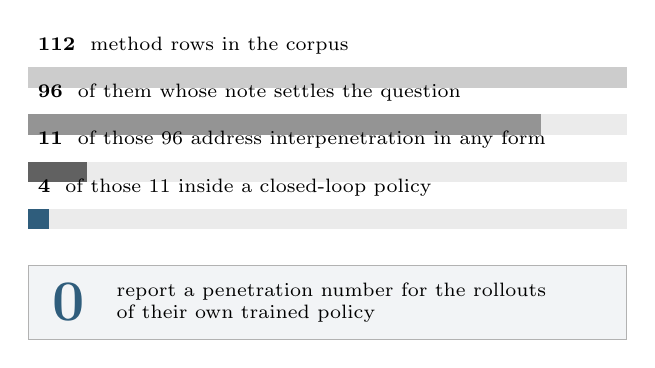
\begin{tikzpicture}[
  font=\footnotesize,
  bar/.style={draw=none,fill=black!62},
  barmid/.style={draw=none,fill=black!42},
  barlight/.style={draw=none,fill=black!20},
  baracc/.style={draw=none,fill=accent},
  seg/.style={draw=white,line width=0.5pt},
  lnk/.style={draw=black!38,line width=0.28pt},
  ghost/.style={draw=black!45,line width=0.3pt,dash pattern=on 1.2pt off 1.2pt},
  lbl/.style={font=\scriptsize},
  small/.style={font=\scriptsize\color{black!55}},
  num/.style={font=\scriptsize\color{black!55}},
]

\node[lbl,anchor=south west] at (0,0.04) {\textbf{112}~~method rows in the corpus};
\fill[black!8] (0,0.00) rectangle (7.60,-0.26);
\fill[barlight] (0,0.00) rectangle (7.60,-0.26);
\node[lbl,anchor=south west] at (0,-0.56) {\textbf{96}~~of them whose note settles the question};
\fill[black!8] (0,-0.60) rectangle (7.60,-0.86);
\fill[barmid] (0,-0.60) rectangle (6.51,-0.86);
\node[lbl,anchor=south west] at (0,-1.16) {\textbf{11}~~of those 96 address interpenetration in any form};
\fill[black!8] (0,-1.20) rectangle (7.60,-1.46);
\fill[bar] (0,-1.20) rectangle (0.75,-1.46);
\node[lbl,anchor=south west] at (0,-1.76) {\textbf{4}~~of those 11 inside a closed-loop policy};
\fill[black!8] (0,-1.80) rectangle (7.60,-2.06);
\fill[baracc] (0,-1.80) rectangle (0.27,-2.06);
\fill[wash] (0,-2.52) rectangle (7.60,-3.46);
\draw[line width=0.3pt,draw=black!30] (0,-2.52) rectangle (7.60,-3.46);
\node[anchor=west,font=\fontsize{22}{22}\selectfont\bfseries\color{accent}] at (0.18,-2.99) {0};
\node[anchor=west,align=left,font=\scriptsize] at (1.00,-2.99) {report a penetration number for the rollouts\\of their own trained policy};
\end{tikzpicture}
}}{%
    \framebox[0.95\columnwidth]{\rule{0pt}{2.2cm}\textit{figs/fig\_penetration.tex pending}}}
  \caption{Interpenetration handling among all \fnRows{} method rows, the settled \fnPenSettled{}
  shown against the light track behind them, split by closed-loop policy versus reference-only
  scoring.}
  \label{fig:penetration}
\end{figure}

The quantity most specific to a hand is the one closed-loop policies do not record, and
\figurename~\ref{fig:penetration} is the funnel that narrows to zero. Eleven method rows handle
interpenetration in any form: three penalise it, three measure it, five constrain it, 11 percent
of the settled rows. The denominator is 96, not 112, because the
contact-handling field is null for 16 rows, and a null there means the note did not settle the
question, not that the paper ignored penetration.

That eleven is not a claim that penetration goes unmeasured in general, and reading it that way
would be wrong. Outside closed-loop control the quantity is a standard comparative column, and has
been one for years in grasp synthesis and in hand-object reconstruction. Four rows of this corpus
show the practice. BiDexGrasp \cite{bidexgrasp_2026} prints a penetration depth beside a prior
method's, BimanGrasp \cite{bimangrasp_2024} fails any grasp that exceeds 1.5 mm of total
penetration, TopoRetarget \cite{toporetarget_2026} reports a maximum penetration and a share of
frames past 2 mm against a baseline retargeter, and OakInk \cite{oakink_2022} scores a dataset
split on penetration depth, solid intersection volume and simulation displacement. The finding is
narrower than the field and concerns learned closed-loop control: all eleven score a pose or a
reference trajectory, four of them are closed-loop policies, and we found none that reports the
measurement for rollouts of its own trained policy.

Where in the pipeline those eleven act is the reference-versus-rollout split that
Section~\ref{sec:intro} takes from \cite{zhao_dexhand_survey_2026}. A reference is a pose or a
trajectory scored before execution, and a rollout is what the trained policy actually did. What
this section supplies on that axis is a measurement method and a count, and it does not supply a
threshold. The count is the eleven of 96 above, with four closed-loop policies inside it and none
we found reporting a number for its own rollouts, which is \figurename~\ref{fig:penetration}. The
method is the plausibility row of Table~\ref{tab:protocol}: maximum and mean penetration depth
over the evaluation rollouts, on a dense surface sample, computed by code that never entered the
reward or the termination rule. The threshold is borrowed, and
Section~\ref{subsec:what_would_be_true} says from where and why it does not bind. Six of the
eleven are grasp synthesisers or trajectory optimisers, namely
\cite{bidexgrasp_2026,bimangrasp_2024,deximit_2026,pang_global_planning_2022,toporetarget_2026}
and \cite{unidexgrasp_2023}, and Castro et al. \cite{castro_sap_contact_2021} give a contact model
rather than a controller. That leaves four closed-loop policies in the whole corpus:
\cite{clutterdexgrasp_2025,dexmachina_2025,dextrack_2025} and \cite{teledexter_2026}.

The reason the number is four is a measurement trap. A quantity a policy optimises cannot also
judge it, because the policy learns the measure rather than the property the measure stands for.
PhysHOI \cite{physhoi_2023} documents the failure in the clean direction. Its kinematic imitation
reward was maximised by not touching the object at all, because contact perturbed the reference
trajectory: ``the policy may learn not to touch the object and falls into a local optimal''. A
contact-graph reward closed the hole, and that reward reads a force threshold rather than
geometry, so it constrains contact presence and says nothing about penetration depth.

DexTrack \cite{dextrack_2025} shows the trap in the other direction. It defines a maximum
hand-object penetration depth over all frames in its Appendix B, and applies it only to the input
kinematic references, as one component of a reference-quality score. No penetration number appears
for any of its own rollouts, in simulation or on the LEAP hand. Tolerance of the failure is then
reported as a result: ``Despite severe hand-object penetrations in Figure 4c and Figure 4a, the
hand still interacts effectively with the object, highlighting the resilience of our tracking
controller''.

TopoRetarget \cite{toporetarget_2026} is the strongest case in the corpus and still stops one step
short on the same reference-versus-rollout line. It constrains penetration during retargeting with
a 1 mm soft tolerance and a 30 mm hard bound, and it reports two numbers on 25 ContactPose grasps:
a maximum penetration of 1.07 mm and 0.00 percent of frames above 2 mm, against 22.22 mm and 96
percent of frames for its GeoRT baseline. Then a PPO controller tracks those references, and its
four reward terms and its five termination criteria govern object pose, link position, joint error
and action smoothness, never penetration. The constrained quantity is the reference, and the
rollout is not re-measured.

Definitions are not shared either. GRAB \cite{grab_2020} estimates contact by proximity, because
``contact cannot be directly observed'', with a 4.5 mm tolerance, and reports that ``\,`Use'
grasps have $3.25 \pm 0.68$ mm average penetration'', without saying whether 3.25 mm is a maximum,
a mean or a median. OakInk \cite{oakink_2022} supplies the fullest published vocabulary:
penetration depth, solid intersection volume and simulation displacement. Its Table 3 scores the
GRAB GrabNet split at 2.53 cm penetration depth, against GRAB's own 3.25 mm. The two differ by a
factor of about eight, and neither source states its distance function precisely enough to
reconcile them, and the two are not scored over the same grasps either, since GRAB's figure is
over its own captured ``use'' grasps and OakInk's is a model's output on the GrabNet split, so a
difference of population and a difference of definition are confounded in the same ratio.

The analytic tradition scored a grasp without simulating it, and Ferrari and Canny's measure
\cite{ferrari_canny_1992} and Roa and Su\'arez's review \cite{roa_suarez_grasp_quality_2015} are
its wrench-space reference points. Neither could be obtained. The first DOI fetch returned HTTP
202 and the second a Springer JavaScript interstitial, so both are cited by metadata only and no
definition here rests on their contents. The learned literature has not replaced that tradition
with anything it measures on its own rollouts. Penetration is a quantity between meshes, so it
needs a simulator or a mesh reconstruction, and the protocol below treats it as a simulation-only
axis.

\textbf{What would close it.} The gap is specific to learned closed-loop control rather than general,
and it is a choice rather than a capability. What would close it is a maximum and a mean penetration
depth over the evaluation rollouts, on a dense surface sample, computed by a measure the policy never
optimised.

\subsection{Statistical practice, and a proposed protocol}
\label{subsec:statistics}

Kress-Gazit et al. \cite{kress_gazit_policy_eval_2024} give the field's reference protocol, and it
prescribes process, not numbers. Write the success criteria before the run and have someone other
than their author score the runs. Match initial conditions with image overlays. Interleave the
policies blind within one session. Report counts rather than percentages, alongside the initial
conditions and the failure modes. Use a posterior over the Bernoulli parameter instead of a point
estimate. It prescribes no minimum trial count anywhere and no frequentist confidence-interval
width anywhere. Its own example report uses 10 initial conditions with two runs each, 20
evaluations per policy, and its worked case shows what 20 buys. Pancake success of 15 of 18
against 11 of 17, nominally 83 against 65 percent, leaves a 0.11 posterior probability that the
worse policy is actually better. At 150 of 180 against 110 of 170 the same rates separate.

The TRI LBM Team \cite{lbm_careful_examination_2025} supplies the missing numbers by fiat rather
than derivation: 50 rollouts per task per policy per condition on hardware, 200 in simulation,
blind, with randomised policy order inside per-initial-condition bundles. It replaces confidence
intervals with Beta-posterior violins and corrects its pairwise tests under Bonferroni, ``unless
otherwise noted''. Its own warning is the strongest sentence in this literature: ``there is
significant risk that many robotics papers are measuring statistical noise due to insufficient
statistical power''.

The rest fall short of their own advice. RoboArena \cite{roboarena_2025} runs 612 double-blind
pairwise comparisons across seven institutions and 4284 rollouts, and reports no confidence
intervals and no per-policy trial counts. The Colosseum \cite{colosseum_2024} evaluates 235 test
sets at 25 episodes each with ``one training seed and one evaluation seed'' per baseline and gives
no intervals in simulation. AutoEval \cite{autoeval_2025} runs 50 trials per policy per task and
calls $\pm 10$ percent ``the natural variance of robot evaluations'', without giving the formula
behind the intervals it plots.

Two papers do give usable numbers. Badithela et al. \cite{suresim_2025} pair real and simulated
trials and de-biases the simulation with a rectifier, saving 20 to 25 percent of hardware trials
at paired correlations of roughly 0.6 to 0.7, and nothing at all at a correlation near zero. The
25 percent figure is the better of its two reported settings, the DP case at $\rho = 0.702$. Its
decision rule is exact: combining helps only when the rectifier variance is below the variance of
the real evaluations. Snyder et al. \cite{beyond_binary_success_2026} give the largest saving. On
the LBM rubrics their sequential test on graded scores cuts simulated evaluation by about 70
percent and hardware by about 45 percent, 286 trials against a nominal 500, with per-task
decisions landing in 12 to 36 paired trials. On RoboArena's data a 30-point gap on continuous
progress scores reaches significance in 18 trials, while a 20-point gap on binary success needs
about 80.

\textbf{A proposed protocol.}\label{subsec:protocol}
Every count below is printed by \path{tools/make_eval_tables.py} in its derivation mode, and each
axis is derived for the statistic that axis actually reports: a single rate takes a Wilson
half-width, a matched comparison takes McNemar, a ratio takes the standard error of the log ratio,
a correlation takes the Fisher-z interval.

Appendix~\ref{app:protocol} works the derivation; what it concludes is the following, and every
count in Table~\ref{tab:protocol} is one of these. A single reported rate takes 100 real rollouts
per cell, because 93 is where the worst-case Wilson half-width of \eqref{eq:wilson} falls to 10
points and 10 points is the coarsest width at which a rate is worth printing. A comparison is a
different question and a harder one. The design is paired, so the count follows McNemar and depends
on the discordance rate rather than on the two rates alone, and separating 50 from 70 percent at
80 percent power takes 57 matched pairs per arm at the assumed discordance of 0.3, which is 114
rollouts against the 186 two independent arms would need. Simulated cells take 200 episodes for a
6.9-point half-width. Perturbation axes are screened at 40 per axis, which ranks the axes and
cannot establish that any one of them hurt, and certified at 101 per arm. Unseen objects resample
the object rather than the trial, at 20 objects and 5 trials each, and a 10-point claim about an
object distribution needs about 93 objects. The transfer axis takes the 100 real trials paired to
100 simulated, and about 457 pairs to separate two correlations 0.1 apart. One hundred is a cap and
not a bill, because a sequential test on a graded score reached its decision in 12 to 36 paired
trials in \cite{beyond_binary_success_2026}, and a cell that stops early reports a confidence
sequence rather than a Wilson interval, never both. The appendix also keeps the counts an earlier
draft of this section quoted and this one withdrew, since the test they were computed for was the
wrong one.

\IfFileExists{tables/table8_protocol.tex}{% alias for table7_protocol.tex; emits once however many sections input it
\ifcsname dxdone@table7_protocol\endcsname\else
  \expandafter\gdef\csname dxdone@table7_protocol\endcsname{}%
  % generated by tools/make_tex_tables.py -- do not edit
\begin{table*}[!t]
\centering
\caption{The proposed evaluation protocol, and this survey's own contribution. No cell is empty: every cell is a proposal.}
\label{tab:protocol}
\footnotesize
\setlength{\tabcolsep}{3pt}
\setlength{\emergencystretch}{1.5em}
\begin{tabular}{>{\raggedright\arraybackslash\hspace{0pt}}p{62pt}>{\raggedright\arraybackslash\hspace{0pt}}p{128pt}>{\raggedright\arraybackslash\hspace{0pt}}p{108pt}>{\raggedright\arraybackslash\hspace{0pt}}p{170pt}}
\toprule
\rowcolor{wash} \hdr{axis} & \hdr{what is measured} & \hdr{minimum trials} & \hdr{reported with it} \\
\midrule
Task success & fraction of episodes meeting a criterion written before the run, and a graded rubric score in $[0,1]$ & 100 real and 200 sim per policy, task and condition for an absolute rate at a 10-point interval; a comparison alone needs 57 matched pairs per arm & raw counts, the criterion verbatim, the rubric, the initial-condition protocol, and an interval whose kind is named \\
Robustness & success under each perturbation axis, and the ratio to the unperturbed anchor & 40 per axis per policy to rank the axes; 101 per axis and 101 at the anchor before any claim that a named axis hurt & both absolute rates with their Wilson intervals, the axis ranges, and the ratio without an interval unless the certifying count was run \\
Unseen objects & mean over held-out objects of per-object success & 20 objects at 5 trials to screen; 93 objects for a 10-point claim & the object list, the per-object rates, a bootstrap interval over objects, and the within-object trial count \\
Physical plausibility & maximum and mean hand-object penetration depth per rollout, and the fraction of frames above 2\,mm & 100 rollouts, simulation only & an interval over rollouts, the sample density, the threshold, the solver's depenetration settings, and at least one rendered rollout \\
Sample and wall-clock cost & environment steps and wall-clock to the checkpoint that produced the headline number & 3 training seeds & the range over seeds, and the statement that 3 seeds is a range and not an interval \\
Real-robot transfer & paired real and simulated outcomes on matched initial conditions, their correlation, and the rectifier variance against the real variance & the 100 real trials paired to 100 sim; about 457 pairs to separate two correlations 0.1 apart & the correlation with its Fisher-z interval, the variance ratio with its bootstrap interval, and which decision the count supports \\
Reproducibility & the released config and checkpoints against the paper's stated objective & not a trial count & the file and line of every disagreement, or an explicit statement that none was found \\
\bottomrule
\end{tabular}
\end{table*}
%
\fi
}{%
  \begin{table}[!t]\centering
    \caption{Pending: the protocol table, generated by the table generator.}
  \label{tab:protocol}
  \framebox[0.95\columnwidth]{\rule{0pt}{1.4cm}}
  \end{table}}

\subsection{The results matrix, and what filling it would cost}
\label{subsec:matrix}

The rows are the 12 most-mentioned dexterous-hand policy methods in the corpus, and the rule is
the one the table's generator implements, stated here in the same words. A candidate is a method
row that names a hand; the hand string must not contain ``parallel'' or ``gripper''; it must carry
at least one paradigm tag that produces a closed-loop policy and must not be a teleoperation
system, because an interface is scored on latency and operator effort rather than on a policy's
success rate. And its name must be at least four characters, so that a short string does not match
everything. Candidates are then scored by the number of other corpus papers whose parsed text
contains the name, and the top 12 by count, ties broken by key, are the rows.

Two corrections changed that ranking. The match is on a whole word. Under the bare substring test
an earlier version used, ``UniDex'' matched inside ``UniDexGrasp'' and ``UniDexGrasp++'', and
\cite{unidex_2026}. A 2026 paper. Sat sixth in a ranking over a corpus written mostly before it,
on 34 mentions that belonged to a different work. As a whole word it has 3 and it is not in the
table. And the interface rule is now applied to every row that carries the tag rather than only to
rows that carry nothing else, which drops \cite{anyteleop_2023} at 34 mentions, \cite{dime_2022}
at 28 and \cite{holo_dex_2022} at 23, along with \cite{dexpilot_2020}, which the earlier prose
already excluded by hand.
%% The counts themselves, generated with the table by tools/make_tex_tables.py. They used to be set
%% under the float in six-point type; they are one sentence of the paragraph that states the rule
%% they follow from.
% generated by tools/make_tex_tables.py -- do not edit
% The mention counts behind the ranking of tables/table8_matrix.tex, as a sentence for the
% body of Section VII, which is where the ranking rule they follow from is stated.
The counts, on whole-word matches over \path{papers/md}, are OpenAI~64; DexMV~50; DAPG~49; DeXtreme~44; DexCap~40; Hora~34; Visual Dexterity~32; Yin et al.~27; UniDexGrasp~27; PDDM~25; HATO~23; DexPoint~22.


The ranking is not one quantity even so. A method's name is taken from the first line of its note,
which yields an acronym for some works and a full title for others, and a title is matched mostly
inside reference lists while an acronym is matched in running text. Those have different base
rates, so the table marks which kind each row was matched on and the two kinds are not comparable
with each other. Mention counts are counts of mentions and not of use, as
Appendix~\ref{app:method} records.

Every cell is empty. This survey re-ran nothing, and no cell can be filled at the denominator
Table~\ref{tab:protocol} asks for. DeXtreme \cite{dextreme_2022} comes closest and is the reason
the claim is stated that narrowly: it reports a criterion, a trial count and an interval. Object
orientation within 0.4 rad of target, $27.8 \pm 19.0$ average consecutive successes with the $\pm$
a 90 percent confidence interval. On 10 trials. The method tabulation is not a counter-example
either, though it looks like one: it carries trial-count, unseen-object, penetration and
code-release columns for all 112 method rows, including all 12 of these. It records what each
method reported. Table~\ref{tab:matrix} asks instead for what Table~\ref{tab:protocol} defines. A
value with an interval, a stated denominator and a criterion written before the run. And no
reported value meets that. The first row of Table~\ref{tab:matrix} is a worked example so that the
format of a cell is unambiguous. Every number in it is fabricated and labelled as such.

\IfFileExists{tables/table9_matrix.tex}{% alias for table8_matrix.tex; emits once however many sections input it
\ifcsname dxdone@table8_matrix\endcsname\else
  \expandafter\gdef\csname dxdone@table8_matrix\endcsname{}%
  % generated by tools/make_tex_tables.py -- do not edit
\begin{table*}[!t]
\centering
\caption{The matrix, for someone else to fill. 12 rows and 84 cells, all 84 of them empty. An empty cell here is not \na: it is a measurement nobody has made, which is the point of the table, and no cell in it has a source to be missing. The first row is a worked example and every number in it is fabricated. Rows are the 12 most-mentioned dexterous-hand policy methods in the corpus, by the rule of Section~VII, scored on whole-word matches over \texttt{papers/md}: \texttt{openai\_\allowbreak dexterity\_\allowbreak 2018}~64; \texttt{dexmv\_\allowbreak 2021}~50; \texttt{dapg\_\allowbreak 2017}~49; \texttt{dextreme\_\allowbreak 2022}~44; \texttt{dexcap\_\allowbreak 2024}~40; \texttt{hora\_\allowbreak 2022}~34; \texttt{visual\_\allowbreak dexterity\_\allowbreak 2022}~32; \texttt{rotating\_\allowbreak without\_\allowbreak seeing\_\allowbreak 2023}~27; \texttt{unidexgrasp\_\allowbreak 2023}~27; \texttt{pddm\_\allowbreak 2019}~25; \texttt{hato\_\allowbreak visuotactile\_\allowbreak 2024}~23; \texttt{dexpoint\_\allowbreak 2022}~22. A mention count is a count of mentions, not of use. $\ast$ marks a work matched on its title rather than on a short name; a title is matched mostly inside reference lists and a short name in running text, so the two kinds of count are not comparable. Each column is an axis of Table~\ref{tab:protocol} and is filled in the units that table asks for.}
\label{tab:matrix}
\footnotesize
\setlength{\tabcolsep}{3pt}
\setlength{\emergencystretch}{1.5em}
\begin{tabular}{>{\raggedright\arraybackslash\hspace{0pt}}p{66pt}>{\raggedright\arraybackslash\hspace{0pt}}p{55pt}>{\raggedright\arraybackslash\hspace{0pt}}p{55pt}>{\raggedright\arraybackslash\hspace{0pt}}p{55pt}>{\raggedright\arraybackslash\hspace{0pt}}p{55pt}>{\raggedright\arraybackslash\hspace{0pt}}p{55pt}>{\raggedright\arraybackslash\hspace{0pt}}p{55pt}>{\raggedright\arraybackslash\hspace{0pt}}p{55pt}}
\toprule
\rowcolor{wash} \hdr{method} & \hdr{task success} & \hdr{robustness} & \hdr{unseen objects} & \hdr{plausibility} & \hdr{cost} & \hdr{transfer} & \hdr{reproducibility} \\
\midrule
\emph{worked example} & 0.72 $\pm$ 0.09 (100) & lighting 0.41 (40), ratio 0.57 & 0.55 [0.41, 0.68], 20 obj & 3.1 / 0.8 mm, 0.12 & 1.2e9 steps, 46 GPU-h & 0.61 [0.47, 0.72] & \texttt{train.\allowbreak yaml:88} \\
\texttt{openai\_\allowbreak dexterity\_\allowbreak 2018}$\ast$ &  &  &  &  &  &  &  \\
\texttt{dexmv\_\allowbreak 2021} &  &  &  &  &  &  &  \\
\texttt{dapg\_\allowbreak 2017}$\ast$ &  &  &  &  &  &  &  \\
\texttt{dextreme\_\allowbreak 2022} &  &  &  &  &  &  &  \\
\texttt{dexcap\_\allowbreak 2024} &  &  &  &  &  &  &  \\
\texttt{hora\_\allowbreak 2022}$\ast$ &  &  &  &  &  &  &  \\
\texttt{visual\_\allowbreak dexterity\_\allowbreak 2022}$\ast$ &  &  &  &  &  &  &  \\
\texttt{rotating\_\allowbreak without\_\allowbreak seeing\_\allowbreak 2023}$\ast$ &  &  &  &  &  &  &  \\
\texttt{unidexgrasp\_\allowbreak 2023} &  &  &  &  &  &  &  \\
\texttt{pddm\_\allowbreak 2019}$\ast$ &  &  &  &  &  &  &  \\
\texttt{hato\_\allowbreak visuotactile\_\allowbreak 2024}$\ast$ &  &  &  &  &  &  &  \\
\texttt{dexpoint\_\allowbreak 2022} &  &  &  &  &  &  &  \\
\bottomrule
\end{tabular}
\end{table*}
%
\fi
}{%
  \begin{table}[!t]\centering
    \caption{Pending: the results matrix, generated by the table generator.}
  \label{tab:matrix}
  \framebox[0.95\columnwidth]{\rule{0pt}{1.4cm}}
  \end{table}}

\textbf{What would have to be true.}\label{subsec:what_would_be_true}
The bill comes first. Per policy and per task the protocol asks for 57 matched trials on the
anchor set, which is the paired count from \S\ref{subsec:protocol}, and 100 on the unseen-object
set, at 20 objects and 5 trials each, with robustness and plausibility absorbed by simulation. A
two-policy comparison on three tasks is then 342 real rollouts on the matched set and 600 on the
unseen-object set, 942 in all, and at one minute per rollout including the reset that is about 16
hours of robot time, before failed resets, repairs and scoring. The same bill computed from the
independent-arm count, which an earlier draft used, was 1200 rollouts and 20 hours. The pairing
removes about a fifth of it rather than the four fifths the pair counts suggest, because a pair is
two rollouts and only the anchor set is paired. AutoEval \cite{autoeval_2025} ran about 850
episodes in 24 hours on a WidowX with three human interventions, and had to pause 20 minutes every
6 hours once the motors overheated. A tendon-driven multi-finger hand is more fragile, so 16 hours
of rollouts is most of a week of calendar time.

That bill is large but not unprecedented. AutoEval \cite{autoeval_2025} records that evaluating
OpenVLA against its baselines took more than 2500 rollouts and more than 100 hours of human labour
across three institutions, and the TRI LBM Team \cite{lbm_careful_examination_2025} analysed about
1800 real rollouts across nine hardware stations. What is unprecedented is paying it for a single
dexterous-hand paper, where the modal per-cell count is 10 trials and the median per-cell count
15, and where the median stated count has been 20 or 22.5 in each of the last three years.

Four things would have to change. Reviewers would have to reward 57 matched trials on one task
over 20 unmatched trials on five, and nothing in the corpus suggests that is happening. The loop
would have to be automated, and AutoEval \cite{autoeval_2025} shows it is buildable for a gripper
at one to three hours of setup, while stating that it supports binary success only and no
robustness axes. Somebody would have to run the penetration measure on their own rollouts, which
is a choice rather than a capability: Section~\ref{sec:sim:engines} shows the depth is computable
from the poses and the meshes in a few lines of Warp, and IsaacGymEnvs already ships a task that
does it every step. An earlier draft of this section made the engine the barrier, and that claim
is withdrawn, because the released code refutes it. And the comparison would have to be
sequential, because the savings in \cite{beyond_binary_success_2026} are the only reason 100 is a
cap rather than a cost.

Four limits apply to the proposal itself. This survey re-ran no method, so every count in
Table~\ref{tab:protocol} is derived from an interval width, a power calculation or another paper's
measurement, and Table~\ref{tab:matrix} is empty because we filled no cell. The counts are
worst-case at $\hat{p} = 0.5$, so a method near 90 percent needs fewer trials for the same width
and a method near 50 percent needs all 100, and the paired count additionally rests on an assumed
discordance of 0.3, which no paper in this corpus reports. The perturbation axes are borrowed from
The Colosseum \cite{colosseum_2024} and SIMPLER \cite{simpler_2024}, which run parallel-jaw
grippers on rigid objects, where SIMPLER found physical parameters moved success rates by at most
15 percent. That is the sensitivity expected to grow with multi-finger contact, and nobody has
measured it. The 2 mm penetration threshold is taken from \cite{toporetarget_2026} with no
independent justification, and the captured human grasps in \cite{grab_2020} sit above it at 3.25
mm, which makes 2 mm a simulator convention rather than a physical bound. So the three things this
survey adds to the reference-versus-rollout axis are a count, a measurement method and a protocol
slot for them, and a threshold is not among them. It is borrowed from one paper and reported as
borrowed, and it will stay a convention until somebody measures penetration on rollouts across
hands and engines and finds a value that separates behaviour a physicist would accept from
behaviour they would not.

\textbf{The methodology literature has no dexterous hand in it.} Seven corpus rows are evaluation
protocols, a small denominator, and not one of them uses a dexterous hand: Badithela et al.
\cite{suresim_2025} run a parallel-jaw gripper and the other six state no hand. Everything proposed
above is therefore assembled from work on grippers and on whole-arm tasks. What would close that, and
close it cheaply, is to run the Table~\ref{tab:protocol} protocol once, on one in-hand reorientation
task with one 16-DoF hand, and release the rollouts as the first row of Table~\ref{tab:matrix}.
%% Section 8. Conclusion.
%% Sections 8 (Gaps) and 9 (Conclusion) were one list of seven claims followed by a narrative that
%% restated four of them. They are one section now: the list is the conclusion's spine, and what
%% followed it keeps only what the list does not say. Both labels are kept, so every cross-reference
%% written against either section still resolves.
%% Converted from paper/sections/08_conclusion.md for the LaTeX edition. The markdown edition in
%% paper/ is a separate edition of the same prose and is not written by this file.
\section{Conclusion}
\label{sec:gaps}
\label{sec:conclusion}

Progress in dexterous manipulation now depends as much on verification as on new methods. The
evidence in this survey supports seven conclusions.

\begin{enumerate}
\item Nine of the 62 method rows that released parseable code state, in a named file at a named
commit, something other than the value their paper prints, and seven further rows have been
withdrawn from that count since its first draft, with two more narrowed.
Table~\ref{tab:codegap} gives each of the nine as a repository, a
commit, a file and two values, and none of their authors was written to before this was posted:
Section~\ref{sec:train:code} says that beside the finding, with the drafted and unsent letters in
\path{outreach/} and the route by which a disputed case is corrected
(Section~\ref{sec:train:code}).

\item No closed-loop policy in the corpus reports interpenetration for the rollouts of its own
trained policy, and every one of the eleven rows that handles penetration at all sits on the
reference side of the reference-versus-rollout split
(Section~\ref{subsec:plausibility}, \figurename~\ref{fig:penetration}).

\item The evaluation-methodology literature this survey builds its protocol on contains no
dexterous hand at all: of its seven corpus rows, one runs a parallel-jaw gripper and the other six
state no hand (Section~\ref{subsec:what_would_be_true}, Table~\ref{tab:protocol}).

\item The generalist and vision-language-action policies that do evaluate on a multi-fingered hand
run it at a median of 6 actuated degrees of freedom, against 16 across the reinforcement-learning
rows that state a count, and the rows reaching the larger band on paper never say whether the hand
was in the evaluation (Section~\ref{sec:train:vla}).

\item Eight hands that can be bought today or built from published designs take zero method rows
between them, while the corpus's experiments concentrate on four designs
(Section~\ref{sec:hands:gap}, \figurename~\ref{fig:hands}).

\item Twenty-one of the 28 rows that put a learned closed-loop controller on two multi-fingered
hands run one policy over a concatenated two-hand observation, a choice compared twice with opposite
outcomes and ablated once (Section~\ref{subsec:coordination}, \figurename~\ref{fig:bimanual}).

\item Human data does not port across hands, and the map is usually unstated: 33 of the 53 method
rows that use human data never say how the human motion reached the robot hand
(Section~\ref{sec:train:human}).
\end{enumerate}

Six concern gaps in the literature. The first concerns publishing practice; the corrections made
during this review are recorded beside the result in Section~\ref{sec:train:code}.

Three of those claims carry a case worth remembering. A reward table in a paper is a claim about a
document, not about a run, and PhysHOI \cite{physhoi_2023} is the instance to keep in mind: the
term its table weights at 0.1 is set to zero in the file at the commit this survey fetched, and
the success criterion the paper reports is itself position-only. Contact is what separates a hand from a gripper, and the obstacle to measuring
it is not the engines. IsaacGymEnvs ships a task that computes a per-environment maximum
interpenetration depth against meshes and gates the policy update on a 1 mm threshold, and Tactile
Genesis \cite{tactile_genesis_2026} offers penetration depth on Genesis geometry as a sensor. The
tooling sits in the field's own benchmark repository and the number is still not reported. DexTrack
\cite{dextrack_2025} has the formula and points it at its inputs. And hardware and software have
come apart on a narrower claim than the hand count first suggests, because 11 of the 19 hands that
take no method row are neither sold nor open and take none for that reason, which is why the fifth
claim is eight hands and not nineteen.

What this survey cannot establish is which method is better than which. It re-runs nothing, and
Section~\ref{sec:evaluation} argues that the published numbers do not compare. Six works are cited
by metadata only, and a seventh, Ma and Dollar 2011, is on disk but unread; no claim rests on any
of them. Every coverage statistic here counts what this survey's extraction captured rather than
what the literature reported. Each is a floor and not a rate, because every miss converts a
reporting paper into a silent one.

Several practical changes require little additional computation. Authors can generate reward
tables from the configurations used for the reported run, cite the exact revision, state the trial
count and success criterion, and release per-trial outcomes. Evaluations can report penetration
depth over policy rollouts as a diagnostic, without optimizing the policy against that measure.
TopoRetarget \cite{toporetarget_2026} shows how informative the result can be. Hardware choices
also deserve a broader base: the Allegro, Shadow, Inspire, and LEAP hands account for most of the
published use in this corpus, while every other listed hand appears in eight method papers or
fewer. Better reporting would make results easier to reproduce; broader hardware coverage would
show which results survive a change of embodiment.


\appendices
%% Appendix A. Method: how the survey was built, and what the method cannot do.
%% Converted from paper/METHOD.md for the LaTeX edition. The markdown edition in paper/ is a
%% separate edition of the same prose and is not written by this file.
%% The appendix letter comes from IEEEtran's \appendices, so no letter is written here.
\section{Method}
\label{app:method}

The survey is written from a corpus that lives on disk. No claim about a paper is made from
memory. Each claim traces to a note, each note to a parsed markdown file, and each markdown file
to a PDF or repository with a recorded hash or commit.

\textbf{Selection.}
Six topic-specific bibliographies were assembled in parallel (simulators and physics, hands and
vendors, reinforcement learning, imitation and human data, bimanual, benchmarks and evaluation),
seeded with the canonical works in each area and extended by search up to 2026-09-17. Every
arXiv identifier was checked by fetching the abstract page and matching the title, and entries
that could not be checked that way are marked. The six lists were merged with deduplication on arXiv
identifier and normalised title, giving 221 entries.

Seven further bibliography entries are not part of that corpus and are not counted anywhere in
this survey. They are the prior audits and case studies Section~\ref{sec:intro} positions this
survey against, they sit in a bibliography of their own as prior work from outside the corpus, and
none of them carries a structured row. No source for them was parsed either, so each is quoted
only from its abstract and its stated method.

\textbf{Acquisition.}
PDFs were downloaded from arXiv or, for work without a preprint, from the publisher or vendor
page recorded in the bibliography. Vendor pages for hands without any paper were fetched as HTML
and converted to markdown, so that a specification quoted in this survey is quoted from a stored
copy of the page and dated. Repositories were shallow-cloned and parsed, then deleted. What
remains is one markdown per repository holding the README, a pruned file tree, the task and
reward configuration files, and the bodies of reward and observation functions.

\textbf{Parsing.}
PDFs were converted with pymupdf4llm, falling back to raw text extraction when the layout parse
returned too little. The corpus manifest records, per entry, the source URL, page count, sha256
of the PDF and the converter used. Two consequences matter for reading this survey. Equations
rendered as images do not survive conversion, so where a reward weight exists only inside a
figure it is recorded as unreadable rather than guessed. Tables are flattened, so a number taken
from a table is quoted with the table it came from and, where the flattening is ambiguous, the
ambiguity is stated.

\textbf{Notes.}
Each entry was read into a structured note under a fixed template: embodiment, learning method,
objective, contact handling, evaluation, reproducibility, stated limitations, and quotable
claims. Notes were written only from the parsed files. Where the source is silent the note says
``not stated'', and nothing was inferred from the reviewer's prior knowledge of the work. For method
papers the reward or loss was quoted from the paper and, separately, from the released code, so
that disagreements between the two are visible rather than smoothed over. Those disagreements
turned out to be common enough to become a finding in their own right.

\textbf{Sources that could not be obtained.}
Six works are cited by metadata only and no claim in this survey rests on their contents. Five
are behind publisher paywalls with no author-hosted copy found on 2026-09-18: Okamura et al.
2000, Bicchi 2000 (IEEE T-RO), Piazza et al. 2019, Roa and Suarez 2015, and Butterfass et al.
2001 on DLR-Hand II. The sixth is Hwangbo et al. 2018 on RaiSim, whose hosted PDF returned no
body. The freely circulating PDF often taken for Bicchi 2000 is a different work, a book chapter,
and is listed separately.

Ma and Dollar 2011 is a seventh case with a different cause. The fetch that failed when its note
was written succeeded on 2026-09-18, so a seven-page PDF and its hash are in the manifest, but no
note has been read from it. It is cited by metadata only for that reason and not because the
source is unavailable.

Three of the 221 bibliography entries carry no structured row. Two are the paywalled Bicchi 2000
and DLR-Hand II entries. The third is \cite{bicchi_grasping_chapter_2001}, which was read into a
note and quoted throughout but is a book chapter rather than a work with an embodiment, a method
or a result to record in a row.

The reference list of this edition is shorter than the corpus, and the two numbers are different
quantities. It prints 205 entries: the 198 corpus entries that some sentence, table or figure of
this paper cites, plus the 7 prior-work entries from outside the corpus. The other 23 corpus
entries carry a row and a note and are counted in every statistic here, but no passage in the paper
names them, so they have nothing to be cited from and do not appear in the list. A reader counting
the reference list should get 205, and a reader counting the corpus should get 221.

\textbf{What this method cannot do.}
Mention counts over the corpus are counts of mentions, not of use: a related-work sentence
counts the same as an experiment. Vendor specifications are manufacturer claims and are labelled
as such throughout, and where a page has since gone offline the note says so. The corpus is
large but not exhaustive, and selection by search favours work that is indexed, in English, and
posted as a preprint. It also favours recent work. Of the 221 bibliography entries, 138 are dated
2024 or later and 16 predate 2018, so this is a corpus of the learned era and any claim here
about a trend over time is a claim about 2022 onward.

Every coverage statistic in this survey measures what this survey's extraction captured, not what
the literature reported. A structured row holds a scalar. A paper that reports a per-task count, a
rubric, or a total spread across several tables produces a null, and a null is then counted as
silence. The bias runs one way. Every miss converts a reporting paper into a silent one, so the
field is made to look worse at reporting than it is. The size of the effect was measured on the
statistic the survey leads with. Of the 34 method rows that had a real robot and no recorded trial
count, 15 carried a count in plain text in their own note, dropped because the paper reports it
per task and the field takes a single integer. Those 15 have since been re-extracted, which moved
the stated-trial-count row from 55 to 70. The success criterion and the unseen-object count were
audited the same way, rising from 79 to 98 and from 32 to 39. What those 19 recovered criteria say is
mostly not a threshold: eleven score by rubric or staged partial credit, five judge binary
completion against a task description by eye, two defer to a benchmark's own definition, and
exactly one, \cite{pistar06_2025}, states a verbatim numeric threshold. The audit counted only
cases where the note itself carried the number, so a count the note also missed is still uncounted,
and 19 trial counts, 8 unseen-object evaluations whose object count the note never gives, and 4
criteria remain genuinely unsettled. Fifteen of the recovered trial counts are named in the rows:
$\pi_0$ \cite{pi0_2024} at ten trials per task, RDT-1B \cite{rdt1b_2024} at 139 across seven
tasks, UMI \cite{umi_2024} at 260, $\pi^{*}_{0.6}$ \cite{pistar06_2025} at 750, Gemini Robotics
\cite{gemini_robotics_2025} at twenty per task, and ten more, which is 44 percent of the audited
nulls and moved the ``never says'' figure from 34 of 89 down to 19. Read
every coverage statistic in this survey as a floor rather than as a rate, and read the bars in
\figurename~\ref{fig:reporting} the same way.

\textbf{The penetration field, audited the same way.} The same mechanism reaches the penetration,
code-release and failure-mode fields. The penetration field has since been audited by hand, because
this survey's second finding is a null over it and a null is worth what the search behind it is
worth. The population is the 85 method rows whose contact-handling field records that the work does
not address penetration. It excludes the 16 nulls, which are already counted as unsettled rather
than as silence, so recovering one would not move the finding. Twenty-five of the 85, 29 percent,
were drawn with \path{random.Random(20260919).sample} over the sorted population, so the draw is
fixed and can be redrawn. Each sampled row was read again in \path{papers/md/}, in its OCR recovery
where one exists, and in \path{code/md/} where a repository was parsed --- and not in
\path{papers/notes/}, because the note is the artefact under suspicion: a field is wrong exactly
when the source says something the note did not carry. A regular expression over the whole source
collected every occurrence of penetration, interpenetration, intersection, intersection volume,
solid intersection, simulation displacement, contact consistency, physical plausibility, signed
distance and contact depth, and of the words that are mistaken for them, and every hit was read in
its context. A row counted as a recovery if its own source reported a measurement of any of those
quantities on that method's own rollouts. A statement that penetration occurs, a citation whose
title says physically plausible, a collision-avoidance constraint on a reference trajectory and a
solver setting did not count, and the three recurring near misses of that kind are listed in
Section~\ref{subsec:plausibility}. Recoveries: none of the 25, against the 20 to 45 percent the
three earlier audits recovered on the fields above. The one-sided 95 percent bound, computed
hypergeometrically over the finite population, is therefore 8 of the 85, and
Section~\ref{subsec:plausibility} states it beside the claim and names the one borderline case that
a reader might count differently. Why this field held where the others did not is visible in the
per-row results: the recovered trial counts and criteria were numbers present in the source and dropped by
a field shaped to hold a scalar, whereas a penetration number is absent from the source altogether.
The earlier audits measured a defect in this schema; this one looked for an absence in the
literature. \path{reviews/penetration_audit.md} holds the seed, the sample and a result per row
beside the sentence it rests on, and \path{tools/audit_penetration.py} redraws the sample and
re-runs the sweep. The code-release and failure-mode fields have still not been audited this way,
and their counts stay floors.

\textbf{Where the tabulation lives.}\label{app:method:tabulation}
Most of this survey's tabulation is not printed in this paper. The 112 method rows, the 21
reward-term objectives scored against their released code inside a 77-row extraction whose ten
columns hold 253 cells no source stated, the 30 teleoperation systems, the 33 hand specifications with the source sentence behind each one, the 15 contact-model
and solver descriptions verbatim, and the sentence behind every cell of the predecessor-survey
comparison: all of it is
reference material, consulted a row at a time and never read through. Printed, it ran to more pages
than the argument it supports. It is in the repository instead.

Read it there in one of three forms. \path{corpus/rows/} holds one JSON record per work, with
every field at full length and no cell cut; this is the form to query, and it is the form every
number in this paper is computed from at build time. \path{paper/tables/} holds the same content
as markdown tables, one file per table, for reading rather than querying. \path{papers/notes/}
holds the structured note each row was read from, with the quotation that supports each field, so
that a cell can be traced to a sentence in a parsed source. The generators are in \path{tools/}:
every table in this paper and in the repository is written by a script there from those records,
so a reader who disagrees with a classification can change it and rebuild rather than argue with a
PDF.

The corpus is not deposited yet, and this paper prints no link to it for that reason. It is
available from the author at the address in the author block, and the archived release will carry a
persistent identifier, which will be the copy to cite for any number quoted here. A survey that
argues for checkable artefacts should point at its artefact rather than reprint it, and a table a
reader cannot recompute is worth less than the record it was compressed from.

Three tables are exceptions and are printed, because the prose reads individual cells out of them
and does not stand up without them: the two hand tables and the engine table, in
Appendix~\ref{app:tables}. The proposed evaluation protocol appears in the body alongside its
justification. Table~\ref{tab:surveys} is the comparison to the fourteen predecessor
surveys, which is this survey's positioning and is therefore set where a reader meets it rather
than in the repository. It prints one of three levels per cell; the sentence supporting each level
remains in the reproducibility materials.

\textbf{Reproduced figures.}
One figure in this edition is not this survey's own artwork. It is a render reproduced from the
paper it discusses, rendered from the stored PDF in the corpus, and it states its source in its own
caption, keyed to the corpus entry it came from and to the page it was taken from. An earlier draft
reproduced eighteen. A plate is kept only where it carries something a drawing cannot, and only
where this paper has the right to print it: a contact defect invisible at the scale of a grasp and
unmistakable at the scale of the contact, on a source that is CC BY 4.0. The other seventeen were
redrawn in the paper's own style or dropped, and what each one was standing in for is said in the
comment at the head of the figure that replaced it, or in the paragraph that absorbed it.
Two of those seventeen went last and for a reason worth stating, because it is a limit on what
this paper shows rather than a tidying of its figures. Both would have needed an author's
permission, since arXiv's non-exclusive licence to distribute grants a third party nothing, and
this paper is posted without asking anyone for anything. One of them argued from geometry and was
redrawn, as \figurename~\ref{fig:retarget}. The other photographed five research hands to scale
beside a human hand and a ruler, and it was dropped rather than redrawn: the honest redraw is a
to-scale outline annotated in millimetres, and no source in the corpus states a hand's length or
its width, so every envelope in such a drawing would have been invented. Section~\ref{sec:hands}
now states that absence instead of illustrating around it.
The one surviving plate is cleared: its source carries CC BY 4.0, read directly from the licence
page on the date the register records, and its caption prints the attribution the licence asks for,
naming the creator, the work, the licence with a link and the change made to the plate. No
permission request and no author email is outstanding, and nothing in this paper waits on a reply.
The register that records, per figure, the licence found, the URL it was read from and the position
it closed at, is \path{tex/PERMISSIONS.md}. The build does not enforce that register.

% generated by tools/make_tex_tables.py -- do not edit
\clearpage
\onecolumn
\scriptsize
\setlength{\tabcolsep}{2pt}
\setlength{\emergencystretch}{2em}
\begin{longtable}{>{\raggedright\arraybackslash\hspace{0pt}}p{92pt}>{\raggedleft\arraybackslash}p{17pt}>{\raggedright\arraybackslash\hspace{0pt}}p{40pt}>{\raggedright\arraybackslash\hspace{0pt}}p{38pt}>{\raggedright\arraybackslash\hspace{0pt}}p{82pt}>{\raggedleft\arraybackslash}p{15pt}>{\centering\arraybackslash}p{12pt}>{\raggedright\arraybackslash\hspace{0pt}}p{52pt}>{\centering\arraybackslash}p{15pt}>{\raggedleft\arraybackslash}p{20pt}>{\raggedleft\arraybackslash}p{24pt}>{\raggedright\arraybackslash\hspace{0pt}}p{34pt}>{\centering\arraybackslash}p{15pt}}
\caption{Every method row in the corpus, 112 of them, on the columns the body version of Table~\ref{tab:methods-top} cuts down to twenty rows. Run across both columns in one-column mode. 221 of the 1232 cells in the 11 columns other than the method and the year (18\%) are \na: no source stated the value.}\label{tab:app-methods}\\
\toprule
\rowcolor{wash} \hdr{method} & \hdr{yr} & \hdr{task} & \hdr{paradigm} & \hdr{hand} & \hdr{DoF} & \hdr{bi} & \hdr{simulator} & \hdr{real} & \hdr{trials} & \hdr{unseen} & \hdr{penetration} & \hdr{code} \\
\midrule
\endfirsthead
\multicolumn{13}{l}{\footnotesize\itshape Table~\ref{tab:app-methods}, continued.}\\
\toprule
\rowcolor{wash} \hdr{method} & \hdr{yr} & \hdr{task} & \hdr{paradigm} & \hdr{hand} & \hdr{DoF} & \hdr{bi} & \hdr{simulator} & \hdr{real} & \hdr{trials} & \hdr{unseen} & \hdr{penetration} & \hdr{code} \\
\midrule
\endhead
\midrule
\multicolumn{13}{r}{\footnotesize\itshape continued on the next page}\\
\endfoot
\bottomrule
\endlastfoot
Ferrari and Canny~\cite{ferrari_canny_1992} & 1992 & \na & \na & \na & \na & \na & \na & \na & \na & \na & \na & no \\
DAPG~\cite{dapg_2017} & 2017 & grasp, reorient, tool+ & RL+demo & ADROIT & 24 & no & mujoco & no & \na & \na & none & yes \\
OpenAI~\cite{openai_dexterity_2018} & 2018 & reorient & RL & ShadowRobot Dexterous Hand & 24 & no & mujoco & yes & 10 & \na & none & no \\
OpenAI~\cite{openai_rubiks_cube_2019} & 2019 & reorient & RL, distil & Shadow Dexterous E Series Hand & 20 & no & mujoco & yes & 10 & \na & none & no \\
PDDM~\cite{pddm_2019} & 2019 & reorient, other & MPC & Shadow Hand & \na & no & mujoco & yes & \na & \na & none & yes \\
DexPilot~\cite{dexpilot_2020} & 2020 & reorient, grasp, tool+ & teleop & Wonik Robotics Allegro hand & 16 & no & \na & yes & 150 & \na & none & no \\
Castro et al.~\cite{castro_sap_contact_2021} & 2021 & bi-coord & \na & Allegro hand & 16 & yes & drake & no & \na & \na & measured & yes \\
DexMV~\cite{dexmv_2021} & 2021 & grasp, tool & RL+demo, data & Adroit Hand & 30 & no & mujoco & no & \na & 500 & none & yes \\
DexPoint~\cite{dexpoint_2022} & 2022 & grasp, other & RL & Allegro Hand & 16 & no & sapien & yes & 260 & 40 & none & yes \\
DeXtreme~\cite{dextreme_2022} & 2022 & reorient & RL & Allegro Hand & 16 & no & isaacgym & yes & 10 & \na & none & yes \\
DexVIP~\cite{dexvip_2022} & 2022 & grasp & RL & Adroit Hand & 30 & no & mujoco & no & \na & \na & none & no \\
Arunachalam et al.~\cite{dime_2022} & 2022 & reorient, grasp & teleop, BC, RL+demo & Allegro Hand & \na & no & mujoco & yes & 10 & \na & none & yes \\
Holo-Dex~\cite{holo_dex_2022} & 2022 & reorient, grasp, tool & teleop, BC & Allegro Hand & 16 & no & \na & yes & 10 & 10 & none & yes \\
Hora~\cite{hora_2022} & 2022 & reorient & RL, distil & Allegro Hand & 16 & no & isaacgym & yes & 240 & 30 & none & yes \\
Predictive Sampling~\cite{mjpc_2022} & 2022 & reorient & MPC & Shadow Hand & \na & no & mujoco & no & \na & \na & none & yes \\
Pang et al.~\cite{pang_global_planning_2022} & 2022 & reorient, grasp, bi-coord+ & trajopt & Allegro Hand & \na & yes & custom convex quasi-dynamic & yes & \na & \na & constrained & yes \\
VideoDex~\cite{videodex_2022} & 2022 & grasp, reorient, tool & BC, data & LEAP Hand & 16 & no & \na & yes & \na & \na & none & no \\
Visual Dexterity~\cite{visual_dexterity_2022} & 2022 & reorient & RL, distil & D'Claw & \na & no & isaacgym & yes & 20 & 12 & none & yes \\
ALOHA~\cite{aloha_act_2023} & 2023 & bi-coord & BC & parallel-jaw gripper & \na & yes & mujoco & yes & 25 & \na & none & yes \\
AnyTeleop~\cite{anyteleop_2023} & 2023 & grasp, tool, handover & teleop, RL+demo & Allegro Hand & \na & no & sapien & yes & 100 & \na & none & yes \\
ArtiGrasp~\cite{artigrasp_2023} & 2023 & grasp, tool, bi-coord & RL & MANO hand model & 51 & yes & raisim & no & \na & 1 & none & yes \\
DexDeform~\cite{dexdeform_2023} & 2023 & bi-coord, other & BC, trajopt & Shadow Dexterous Hand & 28 & yes & plasticinelab & no & \na & \na & none & yes \\
DexPBT~\cite{dexpbt_2023} & 2023 & grasp, reorient, bi-coord & RL & Allegro Hand & 16 & yes & isaacgym & no & \na & \na & none & yes \\
Dexterous Functional Grasping~\cite{dexterous_functional_grasping_2023} & 2023 & tool & RL & LEAP hand & 16 & no & isaacgym & yes & 70 & 5 & \na & no \\
Diffusion Policy~\cite{diffusion_policy_2023} & 2023 & grasp, tool, bi-coord+ & BC, diff & \na & \na & yes & mujoco & yes & 20 & \na & none & yes \\
Dynamic Handover~\cite{dynamic_handover_2023} & 2023 & handover, bi-coord & RL & Allegro Hand & 16 & yes & isaacgym & yes & 15 & 14 & none & no \\
Eureka~\cite{eureka_2023} & 2023 & reorient, bi-coord, other & RL & Shadow Hand & 20 & yes & isaacgym & yes & \na & \na & none & yes \\
Dasari et al.~\cite{pgdm_2023} & 2023 & grasp, tool & RL & ShadowHand & 24 & no & mujoco & yes & \na & \na & none & no \\
PhysHOI~\cite{physhoi_2023} & 2023 & track-ref & RL & SMPL-X humanoid & 90 & no & isaacgym & no & \na & \na & none & yes \\
Robot Synesthesia~\cite{robot_synesthesia_2023} & 2023 & reorient & RL, distil & Allegro Hand & 16 & no & isaacgym & yes & 5 & \na & none & no \\
RotateIt~\cite{rotateit_2023} & 2023 & reorient & RL, distil & AllegroHand & 16 & no & isaacgym & yes & \na & 15 & none & \na \\
Yin et al.~\cite{rotating_without_seeing_2023} & 2023 & reorient & RL & Allegro Hand & 16 & no & isaacgym & yes & 30 & 5 & none & \na \\
UniDexGrasp~\cite{unidexgrasp_2023} & 2023 & grasp & grasp-syn, RL, distil & ShadowHand & 26 & no & isaacgym & no & \na & 241 & penalised & yes \\
UniDexGrasp++~\cite{unidexgrasp_pp_2023} & 2023 & grasp & RL, distil & Shadow Hand & 24 & no & isaacgym & no & \na & \na & none & yes \\
ACE~\cite{ace_teleop_2024} & 2024 & grasp, tool & teleop, BC & Ability Hand & \na & yes & \na & yes & 10 & 18 & none & no \\
AnyRotate~\cite{anyrotate_2024} & 2024 & reorient & RL, distil & Allegro Hand & 16 & no & isaacgym & yes & \na & 10 & none & no \\
AsymDex~\cite{asymdex_2024} & 2024 & bi-coord, grasp & RL & Shadow Hand in simulation & 30 & yes & isaacgym & yes & 20 & \na & none & yes \\
Bidex~\cite{bidex_teleop_2024} & 2024 & bi-coord, handover, tool & teleop, BC & LEAP Hand & 16 & yes & none & yes & 20 & \na & none & no \\
BiDexHD~\cite{bidexhd_2024} & 2024 & tool, bi-coord & RL, distil & LEAP Hand & 16 & yes & isaacgym & no & \na & \na & none & yes \\
BimanGrasp~\cite{bimangrasp_2024} & 2024 & grasp, bi-coord & grasp-syn, diff & Shadow Hand & 22 & yes & isaacgym & no & \na & 225 & penalised & no \\
Bunny-VisionPro~\cite{bunny_visionpro_2024} & 2024 & grasp, tool, bi-coord & teleop, BC & Ability Hand & 24 & yes & \na & yes & 10 & \na & none & yes \\
CyberDemo~\cite{cyberdemo_2024} & 2024 & grasp, reorient, tool & BC, teleop, data & Allegro Hand & 16 & no & sapien & yes & 20 & 2 & none & no \\
DemoStart~\cite{demostart_2024} & 2024 & grasp, tool, reorient+ & RL, distil & DEX-EE Hand & 12 & no & mujoco & yes & 100 & \na & none & no \\
DexCap~\cite{dexcap_2024} & 2024 & grasp, bi-coord, tool & BC, diff, data & LEAP Hand & 16 & yes & none & yes & 60 & 9 & \na & yes \\
DexMimicGen~\cite{dexmimicgen_2024} & 2024 & bi-coord, grasp, tool & data, BC & Inspire dexterous hand & 6 & yes & mujoco & yes & 20 & \na & \na & yes \\
3D Diffusion Policy~\cite{dp3_2024} & 2024 & reorient, grasp, tool+ & BC, diff & Shadow Hand & \na & yes & isaacgym & yes & 40 & 5 & none & yes \\
DrEureka~\cite{dreureka_2024} & 2024 & reorient & RL & LEAP hand & 16 & no & isaacgym & yes & \na & \na & none & yes \\
EgoMimic~\cite{egomimic_2024} & 2024 & grasp, tool, bi-coord & BC & parallel-jaw gripper & 1 & yes & \na & yes & 135 & \na & none & yes \\
GraspXL~\cite{graspxl_2024} & 2024 & grasp & RL & MANO & 45 & no & raisim & no & \na & 503409 & none & yes \\
HATO~\cite{hato_visuotactile_2024} & 2024 & handover, bi-coord & diff & Psyonic Ability Hand & 6 & yes & \na & yes & 10 & \na & none & yes \\
Guzey et al.~\cite{hudor_2024} & 2024 & grasp, tool & RL & Allegro Hand & 16 & no & \na & yes & 10 & \na & none & no \\
HumanPlus~\cite{humanplus_2024} & 2024 & track-ref, loco & RL, BC & Inspire-Robots RH56DFX & 6 & yes & isaacgym & yes & 10 & \na & none & yes \\
Chen et al.~\cite{objdex_2024} & 2024 & track-ref, bi-coord & BC, RL, distil & Shadow Hand & \na & yes & \na & yes & 80 & 1 & none & no \\
OKAMI~\cite{okami_2024} & 2024 & grasp, tool, bi-coord & trajopt, BC & Inspire Hand & 6 & yes & robosuite & yes & 12 & \na & none & yes \\
Omnigrasp~\cite{omnigrasp_2024} & 2024 & grasp, track-ref & RL, distil & SMPL-X whole-body humanoid & 90 & yes & isaacgym & no & \na & 5 & none & yes \\
OmniH2O~\cite{omnih2o_2024} & 2024 & track-ref, loco & RL, distil & Inspire hands & \na & yes & \na & yes & 20 & \na & \na & yes \\
Open-TeleVision~\cite{open_television_2024} & 2024 & bi-coord, tool & teleop, BC & Inspire Robots hand & 6 & yes & none & yes & 20 & \na & none & yes \\
OpenVLA~\cite{openvla_2024} & 2024 & other & VLA & \na & \na & no & libero benchmark & yes & 230 & \na & none & yes \\
PenSpin~\cite{penspin_2024} & 2024 & reorient & RL, distil & Allegro Hand & 16 & no & isaacgym & yes & 50 & 7 & none & yes \\
$\pi_0$~\cite{pi0_2024} & 2024 & other & VLA, flow & \na & \na & yes & \na & yes & 10 & \na & none & yes \\
PianoMime~\cite{pianomime_2024} & 2024 & music & RL+demo, distil & Shadow Hand E3M5 & 23 & yes & mujoco & no & \na & \na & none & yes \\
RDT-1B~\cite{rdt1b_2024} & 2024 & bi-coord & diff & parallel-jaw gripper & \na & yes & \na & yes & 139 & 2 & none & yes \\
ResDex~\cite{resdex_2024} & 2024 & grasp & RL, distil & ShadowHand & 18 & no & isaacgym & no & \na & 241 & none & yes \\
Lin et al.~\cite{twisting_lids_2024} & 2024 & tool, bi-coord & RL & Allegro Hand & 16 & yes & isaacgym & yes & 20 & 15 & none & no \\
UMI~\cite{umi_2024} & 2024 & tool, bi-coord, other & BC, diff, data+ & \na & \na & yes & \na & yes & 260 & \na & \na & yes \\
Atar et al.~\cite{articulated_tools_inhand_2025} & 2025 & tool & RL, BC, distil & Inspire Hand & 6 & no & isaaclab & yes & 50 & \na & none & no \\
Being-H0~\cite{being_h0_2025} & 2025 & grasp, tool & VLA, BC & 6-DoF Inspire hand & 6 & no & \na & yes & 20 & \na & none & yes \\
ClutterDexGrasp~\cite{clutterdexgrasp_2025} & 2025 & grasp & RL, diff, distil & AgiBot dexterous hand & 6 & no & isaacgym & yes & 167 & 2029 & constrained & no \\
He et al.~\cite{cross_embodiment_world_models_2025} & 2025 & other & world, MPC & PSYONIC Ability Hand & \na & no & sapien & yes & 20 & \na & none & no \\
DexGraspVLA~\cite{dexgraspvla_2025} & 2025 & grasp, other & VLA, diff & PsiBot G0-R & 6 & no & \na & yes & 1287 & 360 & none & yes \\
DexMachina~\cite{dexmachina_2025} & 2025 & track-ref, bi-coord & RL & six URDFs: Inspire & \na & yes & genesis & no & \na & \na & constrained & yes \\
DexMan~\cite{dexman_2025} & 2025 & track-ref, bi-coord & RL, trajopt & Shadow Dexterous Hand & \na & yes & isaacgym & no & \na & \na & \na & no \\
DexNDM~\cite{dexndm_2025} & 2025 & reorient & RL, distil & LEAP hand & \na & no & isaacgym & yes & \na & \na & none & no \\
Dexplore~\cite{dexplore_2025} & 2025 & track-ref & RL, distil & Inspire hand & 6 & no & isaacgym & yes & \na & 2 & none & yes \\
DexReMoE~\cite{dexremoe_2025} & 2025 & reorient & RL & GX11 three-fingered dexterous hand & 11 & no & isaacgym & no & \na & 50 & none & no \\
DexterityGen~\cite{dexteritygen_2025} & 2025 & reorient, tool, grasp & RL, diff & Allegro Hand & 16 & no & \na & yes & 240 & \na & \na & no \\
Frau-Alfaro et al.~\cite{dexterous_handover_2025} & 2025 & handover, grasp & RL & Allegro Hand & \na & no & isaaclab & no & \na & 3 & none & \na \\
DexTrack~\cite{dextrack_2025} & 2025 & track-ref & RL+demo & Allegro hand & 16 & no & isaacgym & yes & \na & \na & measured & yes \\
DexUMI~\cite{dexumi_2025} & 2025 & grasp, tool & BC, data & Inspire Hand & \na & no & \na & yes & 20 & \na & \na & yes \\
DexVLA~\cite{dexvla_2025} & 2025 & grasp, tool, bi-coord & VLA, diff & Robotiq parallel-jaw gripper & \na & \na & libero & yes & 10 & 30 & none & yes \\
DexWild~\cite{dexwild_2025} & 2025 & grasp, tool, bi-coord & BC, data & LEAP Hand & 17 & yes & \na & yes & \na & 11 & \na & yes \\
DyDexHandover~\cite{dydexhandover_2025} & 2025 & handover, bi-coord & RL & 11-DoF dexterous hand & 11 & yes & isaaclab & no & \na & 9 & none & no \\
EgoZero~\cite{egozero_2025} & 2025 & grasp, tool & BC & Franka Panda parallel-jaw gripper & 1 & no & \na & yes & 15 & \na & none & yes \\
Gemini Robotics 1.5~\cite{gemini_robotics_15_2025} & 2025 & other & VLA & ALOHA parallel gripper & \na & yes & mujoco & yes & \na & \na & none & no \\
Gemini Robotics~\cite{gemini_robotics_2025} & 2025 & other, handover & VLA, distil & ALOHA 2 parallel gripper & \na & yes & \na & yes & 20 & \na & none & no \\
Geometric Retargeting~\cite{geometric_retargeting_2025} & 2025 & grasp & teleop & Allegro Hand & \na & no & \na & yes & \na & \na & none & yes \\
GR-Dexter~\cite{gr_dexter_2025} & 2025 & bi-coord, grasp & VLA & ByteDexter V2 & 21 & yes & \na & yes & 125 & 23 & none & no \\
GR00T N1.6~\cite{groot_n16_2025} & 2025 & grasp, tool, bi-coord+ & VLA & \na & \na & yes & galaxea r1 pro & yes & \na & \na & none & yes \\
GR00T N1~\cite{groot_n1_2025} & 2025 & grasp, tool, bi-coord+ & VLA, flow & Fourier dexterous hands & \na & yes & robocasa & yes & 10 & 5 & none & yes \\
H-RDT~\cite{h_rdt_2025} & 2025 & grasp, tool, bi-coord & flow & parallel-jaw & \na & yes & robotwin 2.0 & yes & 25 & \na & none & no \\
Helix~\cite{helix_2025} & 2025 & grasp, tool, handover & VLA & \na & \na & yes & \na & yes & \na & \na & none & no \\
Lum et al.~\cite{human2sim2robot_2025} & 2025 & track-ref & RL & Allegro Hand & 16 & no & isaacgym & yes & 70 & \na & none & yes \\
Qiu et al.~\cite{humanoid_policy_human_policy_2025} & 2025 & grasp, tool & BC & Inspire Hand & 6 & yes & \na & yes & 230 & \na & none & yes \\
Lin et al.~\cite{humanoid_sim2real_recipe_2025} & 2025 & grasp, bi-coord, handover & RL, distil & Fourier GR1 hand & 6 & yes & isaacgym & yes & 10 & \na & \na & no \\
ManipTrans~\cite{maniptrans_2025} & 2025 & track-ref, bi-coord & RL, BC, diff & Inspire Hand & 12 & yes & isaacgym & yes & \na & \na & none & yes \\
METIS~\cite{metis_2025} & 2025 & grasp, tool, bi-coord & VLA & Inspire dexterous hand & 6 & yes & \na & yes & 20 & \na & none & no \\
$\pi_{0.5}$~\cite{pi05_2025} & 2025 & other & VLA, flow & \na & \na & yes & \na & yes & 40 & \na & none & yes \\
$\pi^{*}_{0.6}$~\cite{pistar06_2025} & 2025 & other & VLA, RL, flow & \na & \na & yes & \na & yes & 750 & \na & none & yes \\
Goswami et al.~\cite{wm_dex_human_videos_2025} & 2025 & grasp & world, MPC & Allegro Hand & \na & no & robocasa & yes & 12 & \na & \na & no \\
Being-H0.5~\cite{being_h05_2026} & 2026 & bi-coord, other & VLA, flow & Inspire Hand & 6 & \na & libero & yes & 20 & \na & none & yes \\
BiDexGrasp~\cite{bidexgrasp_2026} & 2026 & grasp, bi-coord & grasp-syn, diff & Shadow Hand pair & \na & yes & mujoco & yes & 260 & 30 & measured & no \\
DexImit~\cite{deximit_2026} & 2026 & bi-coord, grasp, tool & data, BC, grasp-syn+ & XHands & \na & yes & \na & yes & \na & \na & constrained & no \\
Dexora~\cite{dexora_2026} & 2026 & grasp, tool, bi-coord & VLA, diff, teleop & XHAND dexterous hand & 12 & yes & mujoco & yes & 20 & \na & none & \na \\
DexTeleop-0~\cite{dexteleop0_2026} & 2026 & grasp, tool, bi-coord & teleop, MPC & Sharpa Wave & 22 & yes & isaacgym & yes & 35 & \na & \na & no \\
EgoScale~\cite{egoscale_2026} & 2026 & grasp, tool, bi-coord & flow, VLA & Sharpa Wave & 22 & yes & \na & yes & 10 & \na & \na & no \\
Zhao et al.~\cite{force_grasp_sim2real_2026} & 2026 & grasp, reorient & RL & xHand & 12 & no & isaaclab & yes & 70 & 2 & \na & no \\
Lin et al.~\cite{poise_2026} & 2026 & reorient & RL & Sharpa Wave hand & 22 & no & isaaclab & yes & 10 & 1 & none & no \\
SimToolReal~\cite{simtoolreal_2026} & 2026 & tool & RL & Sharpa five-fingered hand & 22 & no & isaacgym & yes & 120 & 12 & none & no \\
Li et al.~\cite{teledexter_2026} & 2026 & reorient, tool & RL, teleop & SharpaWave & 22 & no & isaacgym & yes & 15 & \na & penalised & no \\
TopoRetarget~\cite{toporetarget_2026} & 2026 & track-ref & trajopt, RL & Wuji Hand & \na & no & \na & yes & \na & \na & constrained & no \\
UniDex~\cite{unidex_2026} & 2026 & grasp, tool & flow, VLA, data & Inspire & \na & no & \na & yes & 20 & 1 & \na & no \\
ViserDex~\cite{viserdex_2026} & 2026 & reorient & RL, distil & Allegro Hand & 16 & no & isaaclab & yes & 50 & \na & none & no \\
\end{longtable}
\par\vspace{2pt}
\parbox{508pt}{\scriptsize\raggedright \emph{hand} is the first end effector the row names, without the arm it hangs on, and \emph{simulator} is the leading clause of the normalised engine string: both are names, so neither is cut and neither carries an ellipsis. The \texttt{algorithm} field is not printed. It ran to a paragraph a row, which made this table eight pages of ellipses; Section~V describes the algorithms, and \texttt{corpus/rows/} holds that field, the full hand string and the full engine string at their own length.\par}
\twocolumn
\normalsize

% generated by tools/make_tex_tables.py -- do not edit
% Withdrawn from the paper: the design of each protocol measurement and the reason for each count. Appendix E derives every one of them in prose. tools/make_eval_tables.py
% Reference material belongs in the repository, not in the body of a survey that argues
% for checkable artefacts. Appendix A says where the tabulation lives and how to read it.
% This file emits nothing; it exists because a section inputs it by name.


%% Appendix B. The full hand table with its sources.
%% Converted from paper/APPENDIX_B.md for the LaTeX edition. The markdown edition in paper/ is a
%% separate edition of the same prose and is not written by this file.
\section{The full hand table with its sources}
\label{app:hands}

Table~\ref{tab:hands-available} and Table~\ref{tab:hands-announced} split these rows by whether the hand can be bought, and truncate their cells to stay readable. This appendix prints every hand row once and at full width. Nothing here is a measurement by this survey. Every specification is a manufacturer claim, a figure in a paper, or a figure in a press article, and the \texttt{source quality} column says which. Cells reproduce the text stored in the row, with the source's own punctuation and wording.

Table~\ref{tab:hands_full} prints the specifications as the source states them and, beside
them, where each specification came from.

%% tables/hands_full.tex is generated into tex/tables/ by the table generator in tools/.
%% Do not write the table out here; regenerate it there.
\IfFileExists{tables/hands_full.tex}{% generated by tools/make_tex_tables.py -- do not edit
% Stands where the hand-written placeholder for the full hand table with its sources used to be. That placeholder
% set a one-row table reading "Pending generation", which took a table number and
% most of a page. This file emits nothing. \label{tab:hands_full} is attached to
% appendix_hands_full.tex instead, so a reference to it still resolves.
}{%
  \begin{table}[!t]
  \caption{Every hand row at full width, with the provenance of each specification. Pending: generated into \texttt{tex/tables/hands\_full.tex} by the table generator in \texttt{tools/}.}
  \label{tab:hands_full}
  \end{table}}

\noindent\emph{33 rows. 216 of 528 specification cells (40 percent) are values no source stated,
and 31 of 264 provenance cells (11 percent). A blank price is a hand with no public list price
rather than a free hand. \texttt{parsed source in the manifest} gives page count, the first eight
characters of the sha256 of the stored copy, and the date it was fetched. A hand with no manifest
entry was recorded from a page that could not be stored, and its row should be read as a claim
with no retrievable source.}

% generated by tools/make_tex_tables.py -- do not edit
\clearpage
\onecolumn
\scriptsize
\setlength{\tabcolsep}{2pt}
\setlength{\emergencystretch}{2em}
\begin{longtable}{>{\raggedright\arraybackslash\hspace{0pt}}p{50pt}>{\raggedright\arraybackslash\hspace{0pt}}p{70pt}>{\raggedright\arraybackslash\hspace{0pt}}p{96pt}>{\raggedright\arraybackslash\hspace{0pt}}p{72pt}>{\raggedright\arraybackslash\hspace{0pt}}p{80pt}>{\raggedright\arraybackslash\hspace{0pt}}p{52pt}>{\raggedright\arraybackslash\hspace{0pt}}p{66pt}}
\caption{The sentences behind the controlled vocabularies of Tables~\ref{tab:hands-available} and~\ref{tab:hands-announced}, for all 33 hands. 51 of the 198 cells in the 6 description columns (26\%) are \na: no source stated the value. \emph{caveat on the row} is the \texttt{spec\_caveat} field, which is where a figure with no reachable source is named as such; it is empty for a row that carries no caveat rather than for a row nobody checked. Cells are cut at a word boundary where they would otherwise run past the page; \texttt{corpus/rows/} holds every field at full length.}\label{tab:app-hands}\\
\toprule
\rowcolor{wash} \hdr{hand key} & \hdr{maker, in full} & \hdr{actuation, as the source describes it} & \hdr{what the force figure is} & \hdr{tactile, as the source describes it} & \hdr{date of the claim} & \hdr{caveat on the row} \\
\midrule
\endfirsthead
\multicolumn{7}{l}{\footnotesize\itshape Table~\ref{tab:app-hands}, continued.}\\
\toprule
\rowcolor{wash} \hdr{hand key} & \hdr{maker, in full} & \hdr{actuation, as the source describes it} & \hdr{what the force figure is} & \hdr{tactile, as the source describes it} & \hdr{date of the claim} & \hdr{caveat on the row} \\
\midrule
\endhead
\midrule
\multicolumn{7}{r}{\footnotesize\itshape continued on the next page}\\
\endfoot
\bottomrule
\endlastfoot
\texttt{clone\_\allowbreak robotics\_\allowbreak hand\_\allowbreak 2024} & Clone Robotics & hydraulic artificial muscle ('Myofiber' --- small water-filled tubes that contract when pressurized), carbon-fiber bones and ligament-style tethers,\ldots & \na & pressure pads in the palm detect grip firmness (count not given); 70 inertial sensors track angle/speed (proprioception, not\ldots & press, 2025-11-24, on a video of 2025-11-15 & 'under 2 pounds' is an upper bound, and the source does not say whether the 500 W pump and 36 valves are\ldots \\
\texttt{onex\_\allowbreak neo\_\allowbreak hand\_\allowbreak 2026} & 1X Technologies & quasi-direct-drive tendons via the '1X Tendon Drive' at low gear ratios (\textasciitilde{}5:1-15:1); motors in the forearm, tendons pulled through the wrist & distal flexion force, peak vendor claim & high-resolution tactile sensing across fingertips and finger surfaces (normal force, contact location, shear); sensor\ldots & vendor page, 2026-07-09 & \na \\
\texttt{shadow\_\allowbreak dexterous\_\allowbreak hand\_\allowbreak 2005} & Shadow Robot Company & tendon-driven, motors in the forearm (20 Smart Motor nodes, Maxon motors, PWM) & \na & Shadow Tactile Fingertips (STF): 17x3 DoF Hall-effect taxels, 1000 Hz, uncalibrated; up to 5 fingertips; software also supports\ldots & specification dated 2024-12-04 & the four distal joints are coupled and not independently controllable, so the '24 DoF' quoted in learning\ldots \\
\texttt{proception\_\allowbreak prohand\_\allowbreak 2026} & Proception Inc (YC W25) & tendon-driven, motors pull cables to move the fingers & \na & integrated skin-like sensors detecting contact, supporting grip control; same 'sensor skin' used on the companion ProGlove;\ldots & launch post and press, 2026-06-29 & the evidence is a shipping announcement, not a datasheet: no weight, force, actuated-DoF count or control\ldots \\
\texttt{sharpa\_\allowbreak wave\_\allowbreak 2026} & Sharpa Robotics (Sharpa Pte Ltd) & \na & vendor spec table with two unlabelled columns, probably two configurations; grip force is listed separately\ldots & 'Dynamic Tactile Array' (DTA), camera-type array at the fingertip: resolution 240x240 | 60x60, force resolution 0.02 N | 0.05 N,\ldots & undated page, copyright 2026, fetched 2026-09-17 & the page footnotes 'Specifications may vary between products', and no column of the spec table is labelled \\
\texttt{bidexhand\_\allowbreak 2025} & Zhengyang Kris Weng, Center for Robotics and Biosystems, Northwestern University & cable-driven, N-configuration tendon routing (FeeTech servos, endless-loop antagonistic pull-pull); thumb CMC flexion driven via a 4-bar linkage\ldots & fingertip normal force, calibrated sensor, five trials per finger, average peak & none mentioned & paper, 2025 (ICRA Dexterity workshop abstract) & the paper states 16 independently actuated DoF and 21 joints; the README states 15 servos driving 15 joints \\
\texttt{leap\_\allowbreak hand\_\allowbreak v2\_\allowbreak adv\_\allowbreak 2025} & Kenneth Shaw, Deepak Pathak, Carnegie Mellon University & tendon (PIP/DIP coupled by a single tendon per finger); motor type not stated & \na & none mentioned & undated project page; API repo at commit a0936196, fetched\ldots & the page claims 21 DoF with 17 powered motors and the README calls the same hand 17-DOF \\
\texttt{sanctuary\_\allowbreak phoenix\_\allowbreak hand\_\allowbreak 2024} & Sanctuary AI (Sanctuary Cognitive Systems Corporation) & hydraulic, 'unique miniaturized hydraulic valves' & \na & not in the press release text; sidebar-only headlines mention new touch/tactile sensors as a separate later announcement, not\ldots & undated press release; trade reprint 2024-12-17 & \na \\
\texttt{ilda\_\allowbreak hand\_\allowbreak 2021} & Ajou University, Korea Institute of Machinery \& Materials, Korea University & linkage-driven, direct linear drive (3 Maxon DCX8M motors per finger with GPX8 16:1 gearboxes driving ball screws via parallel+serial four-bar\ldots & fingertip normal force in the bent pose; 28 N stretched, and 25 N per finger measured while crushing an\ldots & 6-axis F/T sensor per fingertip (5 total), force resolution 62 mN, range +/-35 N; not a distributed taxel skin & paper, accepted 2021-11-05 & \na \\
\texttt{ruka\_\allowbreak v2\_\allowbreak 2026} & Xinqi (Lucas) Liu, Ruoxi Hu, Alejandro Ojeda Olarte, Zhuoran Chen, Kenny Ma, Charles\ldots & tendon-driven, forearm-mounted actuators; decoupled parallel 2-DoF wrist via a passive spherical ball joint; single-tendon-plus-spring\ldots & \na & optional e-flesh fingertips (magnetic touch-sensing form factor); not part of the base design & paper, 2026 & the AS5600 encoders are attachable and detachable and are read for calibration and measurement only, not in\ldots \\
\texttt{tesollo\_\allowbreak dg5f\_\allowbreak 2024} & Tesollo Inc. (Incheon HQ, Gwangmyeong R\&D/factory) & one integrated actuator per joint ('high-torque actuation', absolute encoder); page does not say direct-drive & \na & none standard; optional fingertip sensors (6-axis F/T, 3-axis force, or tactile) available; count/type not given & undated page, copyright 2026, download links dated 2026-08 & \na \\
\texttt{unitree\_\allowbreak dex5\_\allowbreak 2025} & Unitree Robotics (Yushu Technology Co., Ltd.) & in-joint geared motor ('hollow-cup motor' + high-precision encoder + low-damping small-clearance reducer), backdrivable; page does not use the words\ldots & fingertip normal force under a 1 cm diameter cylinder pressed vertically down (vendor footnote) & Dex5-1: none. Dex5-1P: 94 pressure sensors per hand (2x5 palm + 2x3x5 finger pad + 2x3x5 fingertip + 2x3x4 finger root), range 10\ldots & undated page, copyright 2016-2025, fetched 2026-09-17 & \na \\
\texttt{wuji\_\allowbreak hand\_\allowbreak 2025} & Wuji Technology (founded 2019) & direct-drive rotary, backdrivable & \na & 'Multi-Axis Force/Torque Fingertip Sensing' confirmed present; no type, count or range given & undated page, copyright 2026, fetched 2026-09-17 & the page footnotes that these figures 'reflect the current Beta1 product and the SPEC will continue to\ldots \\
\texttt{pisa\_\allowbreak iit\_\allowbreak softhand\_\allowbreak 2014} & Centro E. Piaggio, University of Pisa and IIT (Catalano, Grioli, Farnioli, Serio, Piazza,\ldots & tendon-driven adaptive synergy, single motor via differential gears (6 W Maxon RE-max21, 84:1 reduction) & \na & none (motor encoder only; a padded work glove supplied contact compliance during experiments) & paper, IJRR 2014 & \na \\
\texttt{orca\_\allowbreak hand\_\allowbreak 2025} & Clemens C. Christoph, Maximilian Eberlein, Filippos Katsimalis, Arturo Roberti,\ldots & tendon-driven (antagonistic fishing-line tendon pairs per joint); wrist uses a GT2 timing belt drive & \na & yes: FSR-based binary tactile sensing on all 5 fingertips (RP-C7.6-ST), absolute detection threshold as low as 0.05 N & paper, 2025 & the 19.6 N previously tabulated as a fingertip force is the newton equivalent of the 2 kg index-finger\ldots \\
\texttt{allegro\_\allowbreak hand\_\allowbreak v4\_\allowbreak 2016} & Wonik Robotics Co. Ltd. (Seoul, South Korea); earlier versions 1.0/2.0 made by SimLab Co.\ldots & \na & \na & none & driver repo, versions 1.0-4.0 undated, fetched 2026-09-17 & allegrohand.com/v4 returned HTTP 404 and the Wonik wiki timed out; every cell here comes from the ROS driver\ldots \\
\texttt{faive\_\allowbreak hand\_\allowbreak 2023} & Yasunori Toshimitsu, Benedek Forrai, Barnabas Gavin Cangan, Ulrich Steger, Manuel Knecht,\ldots & tendon-driven, rolling-contact joints (16 Dynamixel XC330-T288-T servos, 6 antagonistic pairs) & \na & none on the physical hand; a simulated 'fingertip force' (15-dim, critic-only/privileged) exists only in the RL training\ldots & paper, 2023 & the row's open-hardware status is unconfirmed: the repo has LICENSE and LICENSE-NVIDIA files whose contents\ldots \\
\texttt{leap\_\allowbreak hand\_\allowbreak 2023} & Kenneth Shaw, Ananye Agarwal, Deepak Pathak, Carnegie Mellon University & direct-drive (Dynamixel servos, e.g. XC330-M288), joint velocity \textasciitilde{}8 rad/s & pull-out resistance: the outward force a flexed finger resists before slipping or deviating more than 15\ldots & none (future work only: 'we plan to develop and integrate LEAP Hand with low-cost touch sensors') & paper, 2023 & \na \\
\texttt{ruka\_\allowbreak 2025} & Anya Zorin, Irmak Guzey, Billy Yan, Aadhithya Iyer, Lisa Kondrich, Nikhil X. Bhattasali,\ldots & tendon-driven (11 Dynamixel actuators in the forearm: XM430-W210T for the thumb, XL330-M288-T for the other fingers) & pinch force, best of three trials, averaged over the left and right hands (Table III) & none (stated limitation: 'lacks tactile sensing') & paper, 2025 & \na \\
\texttt{inspire\_\allowbreak rh56dfx\_\allowbreak 2023} & Beijing Inspire Robots Technology Co., Ltd. & \na & fingertip strength, vendor spec, four fingers; thumb 15 N; force resolution 0.50 N & none (this variant is the 'without tactile sensors' table; a tactile FTP variant exists per bib but is not on this page) & undated page, fetched 2026-09-17 & the vendor's own page reads 'Degrees of freedom 6, Numbers of joints 12'; the joints column here prints the\ldots \\
\texttt{robotera\_\allowbreak xhand1\_\allowbreak 2024} & ROBOTERA & gear-driven force-controlled joint modules per finger segment, back-drivable & \na & tactile/force sensors on every fingertip confirmed present (senses contact, force, temperature); count and array size not stated & undated tracker page, fetched 2026-09-17; the vendor page\ldots & the 15 N in circulation comes from a survey table, not from the tracker or the vendor; the tracker states no\ldots \\
\texttt{shadow\_\allowbreak dex\_\allowbreak ee\_\allowbreak 2024} & Shadow Robot Company, in collaboration with Google DeepMind & \na & \na & stereo camera-based fingertip tactile sensors (hundreds of taxels each); multi-taxel 3-DoF arrays on middle and proximal\ldots & undated page, copyright 2026, fetched 2026-09-17 & \na \\
\texttt{brainco\_\allowbreak revo2\_\allowbreak 2025} & BrainCo Inc. & \na & pinch force, vendor minimum (>=15 N); the same page states a whole-fist grip of >=50 N & Touch variant only: multi-dimensional fingertip tactile module with 'Tactile Adaptive Control'; count/type not stated. Basic and\ldots & undated page, fetched 2026-09-17 & \na \\
\texttt{agibot\_\allowbreak omnihand\_\allowbreak 2025} & \na & \na & \na & \na & no source: both store.agibot.com URLs 404, fetched\ldots & \na \\
\texttt{boston\_\allowbreak dynamics\_\allowbreak atlas\_\allowbreak hand\_\allowbreak 2026} & Boston Dynamics & electric (robot is fully electric); specific hand mechanism not stated & \na & tactile sensing in the fingers and palms, confirmed present; type and count not stated & trade press, 2026-01-05 (CES); the Boston Dynamics blog of\ldots & \na \\
\texttt{daxo\_\allowbreak muscle\_\allowbreak v0\_\allowbreak 2025} & Daxo Robotics & ultra-redundant tendon-driven; compliant structure with no rigid joints, flexible materials and tendon routing & \na & \na & third-party catalogue post, 2026-09-16; daxo-robotics.com\ldots & 120 actuators in 750 g is about 6 g per actuator including structure, tendons, routing and skin; no DoF\ldots \\
\texttt{dexhand\_\allowbreak open\_\allowbreak source\_\allowbreak 2023} & Rob Knight, The Robot Studio (design); electronics/firmware/ROS 2 by Trent Shumay, IoT\ldots & tendon (fishing line, Sufix 832 80lb / 0.8mm kiteline); Emax ES3301/ES3302/ES3351/ES3352 micro-servos for fingers, Feetech SCS2332 or PWM servos for\ldots & \na & none mentioned & page posts 2023-08-08 to 2023-10-01; no hardware release\ldots & no joint count is given anywhere, so no DoF figure can be quoted; the servo count is 16 finger and thumb\ldots \\
\texttt{figure\_\allowbreak 03\_\allowbreak hand\_\allowbreak 2025} & Figure AI & \na & \na & not stated on page for the hand itself; palm cameras in each hand are vision, not tactile & undated tracker page, fetched 2026-09-17; figure.ai launch\ldots & the tracker's 'Degrees of freedom, hands | 20' sits beside 'Number of fingers | 10', so the 20 is most likely\ldots \\
\texttt{linkerbot\_\allowbreak l20\_\allowbreak 2025} & LinkerBot (SDK author 'CHIUS INC') & \na & \na & L10/L20: per finger 4 channels (normal force, tangential force, tangential direction, proximity), 5 sites x 4 channels, 0-255\ldots & undated page, fetched 2026-09-17 & \na \\
\texttt{paxini\_\allowbreak dexh13\_\allowbreak 2024} & PaXini Tech & \na & \na & 1,140 ITPU multidimensional tactile processing units (press-release claim; unclear if PX-6AX-GEN3 sensor family) & press, CES 2026-01-07 & \na \\
\texttt{psyonic\_\allowbreak ability\_\allowbreak hand\_\allowbreak 2021} & PSYONIC (San Diego, CA, USA) & linkage (repo file/function names indicate a four-bar finger linkage; not stated on the vendor page itself) & \na & 30 touch sensor values streamed (FSR-based per API and URDF 'no\_fsr' variant); per-finger split not stated & undated page, fetched 2026-09-17 & the four-bar finger linkage rests on repository file names and the five fingers on URDF meshes; the vendor\ldots \\
\texttt{tesla\_\allowbreak optimus\_\allowbreak hand\_\allowbreak 2025} & Tesla & V3: tendon-driven from forearm actuators, three tendons per finger through a crosstalk-managing wrist. Gen 2: in-hand actuators/sensors (unlocated in\ldots & \na & Gen 2: tactile sensing on all fingers, demonstrated matching contact location and force in an egg-pickup video; type/count not\ldots & Gen 2 video 2023-12-13; V3 patents filed 2024-10, relayed\ldots & the 22 DoF in circulation is a Teslarati article's arithmetic of four DoF on each of five fingers plus two at\ldots \\
\texttt{xiaomi\_\allowbreak cyberone\_\allowbreak hand\_\allowbreak 2026} & Xiaomi & motors located in the hand (compact motors generate heat requiring liquid cooling); no tendon/linkage statement, though contrast with tendon-driven\ldots & \na & full-palm tactile sensing, area \textasciitilde{}8,200 sq mm, detects pressure and contact across the whole palm not just fingertips; taxel count\ldots & press, 2026-03-30 & \na \\
\end{longtable}
\twocolumn
\normalsize


%% Appendix C. Per-paper reward term extraction.
%% Converted from paper/APPENDIX_C.md for the LaTeX edition. The markdown edition in paper/ is a
%% separate edition of the same prose and is not written by this file.
%% Every table number inside the disagreement entries is the cited paper's own table, so
%% those stay literal numbers. Our own tables are cross-referenced.
\section{Per-paper reward term extraction}
\label{app:rewards}

Table~\ref{tab:rewards} marks nine recurring term families across the in-hand reorientation methods. This appendix is the extraction underneath it, over every method row that records a reward at all. \texttt{terms stated} counts the terms the paper itself names. \texttt{where the reward was read} gives the section of the paper or the file in the released code that the note quotes. A row with a \texttt{paper/code class} is one where the two disagree, and the second part of this appendix prints the disagreement in full. Cells and entries reproduce the text stored in the row, with the source's own punctuation and wording.

\subsection{The extraction}

%% tables/rewards_full.tex is generated into tex/tables/ by the table generator in tools/.
%% Do not write the table out here; regenerate it there.
\IfFileExists{tables/rewards_full.tex}{% placeholder: generated by tools/make_tex_tables.py, not yet written
\begin{table}[t]
\caption{Appendix table \texttt{rewards\_full}. Pending generation.}
\label{tab:rewards_full}
\centering\footnotesize
\begin{tabular}{l}
\toprule
This table is generated from \texttt{corpus/rows} and is not yet written.\\
\bottomrule
\end{tabular}
\label{tab:app-contact}
\end{table}
}{%
  \begin{table}[!t]
  \caption{The per-paper reward term extraction, over every method row that records a reward at all. Pending: generated into \texttt{tex/tables/rewards\_full.tex} by the table generator in \texttt{tools/}.}
  \label{tab:rewards_full}
  \end{table}}

\noindent\emph{77 rows. 253 of 770 cells (32 percent) are values no source stated. A blank \texttt{terms stated} with a filled \texttt{term names} column is a paper that names its terms without numbering them. \texttt{in Table 5} marks the rows that are also in the body matrix, which covers in-hand reorientation only.}

\subsection{Paper against released code, in full}
\begingroup\sloppy
\emergencystretch=3em

Each entry below is the disagreement text stored in the row, unedited. The class is what Sec. 5.8 and Sec. 8.1 count. \texttt{contradiction} means the paper states one value and the shipped code demonstrably states another. \texttt{parse-limitation} means this survey's own parse could not settle it and the accusation is withdrawn. \texttt{code-absent} means the described component is not in the released repository. \texttt{version-skew} means the repository is a later generation than the paper. \texttt{internal-inconsistency} means the paper disagrees with itself and no code is implicated.

\textbf{contradiction, 10 rows.}

\begin{itemize}
\item PDDM \cite{pddm_2019} (high). Table 2 states obs-dim 46 for In-hand Reorientation while the released cube\_\allowbreak{}env.py code sums to 39; the Baoding reward code includes an extra -10*wrist\_\allowbreak{}too\_\allowbreak{}high term absent from Table 2's printed formula.
\item DexPoint \cite{dexpoint_2022} (high). The released code's reward adds several terms absent from the paper's four-term Eq. 5 (a lift-threshold bonus, a target-distance term, a rotation bonus, and an IK controller-tracking penalty) and reshapes the reach/lift terms into inverse-distance and clipped forms rather than the paper's plain distance/height-difference formulas.
\item DeXtreme \cite{dextreme_2022} (high). Action Delta Penalty weight is -0.25 in paper Table 2 but -0.2 in the ADR yaml and -0.01 in the ManualDR yaml; the Joint Velocity Penalty in code normalises velocity by (max\_\allowbreak{}velocity-vel\_\allowbreak{}tolerance) unlike the paper's stated formula; code has a timeout\_\allowbreak{}rew term absent from the paper's reward table; Appendix Table 12 states critic learning rate 5e-4 and KL threshold 0.16, vs body text/code values of 5e-5 and 0.016.
\item Visual Dexterity \cite{visual_dexterity_2022} (high). Table S1 states 32000 teacher training environments, but the released config sets alg.num\_\allowbreak{}envs to 8000 (parent config 16384); fallDistance differs across two shipped configs (0.24 vs 0.15, only the latter matching Table S1's threshold); the paper's Eq 8 penultimate-joint penalty (c7=-2) does not appear anywhere in the released reward code; the config carries a dead distRewardScale=-10.0 key never used in compute\_\allowbreak{}reward; and the paper's table-friction lower bound (0.05) differs by a factor of 10 from the code's randomized lower bound (0.005).
\item DexPBT \cite{dexpbt_2023} (high). Paper presents the reward as 4 mutually exclusive stage terms (r\_\allowbreak{}reach, r\_\allowbreak{}pick, r\_\allowbreak{}targ, -r\_\allowbreak{}vel), but code's compute\_\allowbreak{}kuka\_\allowbreak{}reward sums 8 named components, one of which (hand\_\allowbreak{}delta\_\allowbreak{}penalty) is multiplied by 0 and disabled; there is no single r\_\allowbreak{}vel term in code, instead separate kuka/allegro action penalties whose exact formula is not shown. Also, the paper reports zero experiments with domain randomization, yet the shipped AllegroKuka.yaml already carries a fully specified DR schedule (disabled via randomize: False).
  \\ \emph{Review:} R3 adversarial review: the disabled-randomisation half is withdrawn, since the note finds it consistent with the paper; the zeroed reward term stands
\item PhysHOI \cite{physhoi_2023} (high). The released code hardcodes the body position-velocity error and the object rotation/rotation-velocity errors to zero in compute\_\allowbreak{}humanoid\_\allowbreak{}reward, so despite Table 4 listing nonzero $\lambda^{or}$=0.1/$\lambda^{orv}$=0.01 weights for GRAB, the trained reward never actually tracks object orientation (position-only in practice).
\item UniDexGrasp \cite{unidexgrasp_2023} (high). The paper describes a four-term weighted reward (r\_\allowbreak{}goal + r\_\allowbreak{}reach + r\_\allowbreak{}lift + r\_\allowbreak{}move via Table 7's omega weights) but the released compute\_\allowbreak{}hand\_\allowbreak{}reward implements a different threshold-gated torch.where cascade with distinct hardcoded coefficients that do not map one-to-one onto the paper's weights.
\item OmniH2O \cite{omnih2o_2024} (medium). stumble weight -0.00125 (paper) vs -1250 (code); max-feet-height sign/magnitude differ (+1000 paper vs -2500 code, a penalty not a bonus); paper's exp(-c*//.//) form vs code's exp(-err$^{2}$/sigma); curriculum level-down threshold 40 (paper) vs 50 (code)
  \\ \emph{Review:} R3 adversarial review: plausible alternative reading; held at medium confidence pending a direct code read
\item PenSpin \cite{penspin_2024} (medium). The released code disables the paper's tactile observation channel and zeroes the described disturbance-force domain randomization, and the code's reward scale-key names (e.g. rotate\_\allowbreak{}reward\_\allowbreak{}scale, pencil\_\allowbreak{}z\_\allowbreak{}dist\_\allowbreak{}penalty\_\allowbreak{}scale) do not 1:1 name-match the paper's Table 4 weight list, though matched values agree.
  \\ \emph{Review:} R3 adversarial review: plausible alternative reading; held at medium confidence pending a direct code read
\item PianoMime \cite{pianomime_2024} (high). Paper's Table 3 states 2 weighted reward terms (Key Press 2/3, Mimic 1/3), but the released code sums roughly 5 unweighted terms (key press doubled, sustain, energy and fingering hardcoded to return 0, forearm-collision) plus a separately-added mimic wrapper term.
\end{itemize}

\textbf{internal-inconsistency, 3 rows.}

\begin{itemize}
\item ALOHA \cite{aloha_act_2023} (high). Algorithm 1 pseudocode states L\_\allowbreak{}reconst = MSE, but Sec.IV.C's prose explicitly states L1 loss is used instead; the algorithm box and the implementation text disagree; code/md captures only function signatures, not bodies, for policy.py's loss implementation
\item 3D Diffusion Policy \cite{dp3_2024} (medium). the paper's prose states the network predicts the noise added to the data, but the shipped default config trains with prediction\_\allowbreak{}type: sample (predicting the denoised action a$^{0}$ directly), not epsilon; the paper only qualifies this later in the same section (Fig. 7 ablates both).
\item DexMachina \cite{dexmachina_2025} (low). paper describes a plain weighted sum lambda\_\allowbreak{}task*r\_\allowbreak{}task + lambda\_\allowbreak{}imi*r\_\allowbreak{}imi + lambda\_\allowbreak{}bc*r\_\allowbreak{}bc + lambda\_\allowbreak{}con*r\_\allowbreak{}con with unspecified weights; code implements a multiplicative task term with per-component beta decay, an unmentioned 0.1 force-penalty term, and curriculum-driven decay of auxiliary weights not described as such in the paper
  \\ \emph{Review:} R3 adversarial review: the multiplicative form credited to the code is printed in the paper itself
\end{itemize}

\textbf{version-skew, 4 rows.}

\begin{itemize}
\item Hora \cite{hora_2022} (high). The parsed code commit's joint-noise range, disabled default disturbance force, and default cube object type differ from the paper's stated values; the code README itself says to use tag v0.0.1, not the parsed commit, to reproduce paper numbers.
\item $\pi_0$ \cite{pi0_2024} (high). The released repo (openpi, commit 215abfb2) has evolved past this paper: it also documents pi0-FAST (autoregressive) and pi0.5 checkpoints/configs not described in this paper, which describes only the flow-matching pi0 and the non-VLM pi0-small ablation.
\item GR00T N1.6 \cite{groot_n16_2025} (high). code/md is the current Isaac-GR00T main branch (N1.7 generation, commit 51d4c89f), not the N1.6 checkpoint; the repo names a separate n1d6 branch for N1.6 that was not fetched. The page states N1.6's backbone is ``an internal NVIDIA Cosmos-2B VLM variant,'' but the repo's own changelog states the Eagle backbone (nvidia/Eagle-Block2A-2B-v2) was used through N1.6 and only replaced by Cosmos-Reason2-2B in N1.7 -- whether the page's Cosmos-2B variant is a third distinct model or the page is describing N1.7 under an N1.6 headline is not resolvable from what was fetched.
  \\ \emph{Review:} The page attributes a Cosmos backbone to N1.6 while the repository changelog says N1.6 used Eagle and N1.7 made the switch, so the repository is a later generation than the page describes.
\item GR00T N1 \cite{groot_n1_2025} (high). The parsed code repo (Isaac-GR00T, commit 51d4c89f) is a later N1.7 generation, not the paper's GR00T-N1-2B: VLM backbone changed from the paper's Eagle-2 to Cosmos-Reason2-2B (via Qwen3-VL); action horizon expanded from the paper's stated H=16 to 40; state/action dimensions expanded from 29 to 132; DiT layers changed from 32 to 16; embodiment scope widened to include Unitree G1, AgiBot G1, and a `YAM' arm not described in the paper.
\end{itemize}

\textbf{code-absent, 8 rows.}

\begin{itemize}
\item AsymDex \cite{asymdex_2024} (medium). Code contains a GraspAndPlace-task reward variant (AllegroHandDualArmGraspAndPlaceAsymDex.py) with exponential hand-distance and block-alignment terms not one of the four BiDexHands tasks described in the paper body.
\item DexMimicGen \cite{dexmimicgen_2024} (high). The environment code includes an unused `reward\_\allowbreak{}shaping' branch (if self.reward\_\allowbreak{}shaping: pass) that is never described or used in the paper text; only the sparse binary completion reward is used, as the paper states.
\item DrEureka \cite{dreureka_2024} (high). The released DrEureka repo (code/md) contains only forward\_\allowbreak{}locomotion/ and globe\_\allowbreak{}walking/ trees; the LEAP-hand cube-rotation training/deployment code and the quoted Prompt-13 reward are the LEAP-hand authors' own code, not included in the released repo, so the cube-rotation reward cannot be cross-checked against a code file.
\item Open-TeleVision \cite{open_television_2024} (low). The paper's prose states 25k training iterations, lr 5e-5, batch size 45, but the code repo's example training command instead shows 50000 epochs and an explicit kl\_\allowbreak{}weight=10 not mentioned anywhere in the paper text.
  \\ \emph{Review:} R3 adversarial review: a behaviour-cloning paper with no reward; the charge compared paper iterations to a README example's epochs
\item Being-H0 \cite{being_h0_2025} (high). The actual downstream action-head module referenced in \S4.3 (learnable query tokens, proprioceptive projector f\_\allowbreak{}p, regression head f\_\allowbreak{}r) is not present in the parsed code; the repo's own TODO list marks `Training code and scripts' as unreleased, so the action-chunk-length=16 value and exact proprioception-vector fields come only from inference/eval CLI examples, not a verifiable implementation.
\item $\pi_{0.5}$ \cite{pi05_2025} (high). The paper describes a hybrid discrete-FAST-token-pretrain-then-flow-matching-post-train recipe (Eq. 1, alpha: 0 to 10), but the released repo states plainly it `currently only support[s] the flow matching head for both pi0.5 training and inference.'
\item $\pi^{*}_{0.6}$ \cite{pistar06_2025} (high). The general openpi framework (pi0/pi0.5/FAST, flow-matching action head, ALOHA/DROID/LIBERO adapters) is released at commit 215abfb2, but the RECAP-specific pieces described in the paper -- the advantage-conditioning input, the distributional value function, the RECAP training loop (Algorithm 1), and the espresso/laundry/box-assembly checkpoints and datasets -- are not present in the parsed repo.
\item Being-H0.5 \cite{being_h05_2026} (high). Released code (commit e12ac44f) exposes only benchmark/inference/config scaffolding (policy.py, beingh\_\allowbreak{}policy.py, dataset-transform configs). no MoT/MoF model definition, no rectified-flow action-expert source, and no config for any dexterous-hand embodiment; the only post-train configs present (libero\_\allowbreak{}robocasa.yaml, libero\_\allowbreak{}all.yaml, robocasa\_\allowbreak{}human.yaml, so101\_\allowbreak{}example.yaml) are all gripper-only, so the dexterous-hand claims cannot be cross-checked against released code.
\end{itemize}

\textbf{parse-limitation, 13 rows.}

\begin{itemize}
\item ArtiGrasp \cite{artigrasp_2023} (low). paper's two regulariser weights (w\_\allowbreak{}rh=0.5, w\_\allowbreak{}ro=0.2) correspond to five separate velocity penalties in code (-0.5,-0.2,-0.5,-0.5,-0.3); the fingertip weight 12.0 and lambda 5.0 in Table 6 do not appear in the yaml; reward weights differ between curriculum phase-1 and phase-2 configs though Table 6 reports only one set
  \\ \emph{Review:} R3 adversarial review: the reward body is C++ and absent from the parse; the weight split is the paper's documented curriculum
\item Diffusion Policy \cite{diffusion_policy_2023} (high). the paper's core loss equations (DDPM training loss, EBM/InfoNCE, score-matching) are unrecovered images in the parsed text, and code/md is a signature-only API map, so compute\_\allowbreak{}loss's body could not be verified from code; only the exact shipped noise-scheduler config (DDPMScheduler, 100 train steps) is confirmed.
\item Eureka \cite{eureka_2023} (low). The released repo's default eureka/cfg/config.yaml ships iteration:1, sample:3 (a fast-test default), not the paper's reported experimental configuration of N=5 iterations $\times$ K=16 samples $\times$ 5 independent runs, and LLM-generated reward code itself is never checked into the repo (written at runtime to a gitignored outputs/ directory).
  \\ \emph{Review:} R3 adversarial review: the repo README documents the paper's defaults; the cited config block is a fast-test preset
\item UniDexGrasp++ \cite{unidexgrasp_pp_2023} (low). The paper's four named reward weights (0.5, 0.1, 2, 10) numerically match literals in the released compute\_\allowbreak{}hand\_\allowbreak{}reward, but the code never labels them with the paper's variable names, and the paper's own display equations were dropped from the PDF, so the correspondence is inferred rather than confirmed by either source.
\item BiDexHD \cite{bidexhd_2024} (high). Table 5 weights (w\_\allowbreak{}r, w\_\allowbreak{}t, w1-w4, lambda\_\allowbreak{}w=0.12, lambda\_\allowbreak{}ft=0.48) cannot be matched to code reward lines because the code md truncates the reward function before stage-2/final sum; lambda\_\allowbreak{}w and lambda\_\allowbreak{}ft numerically match the code's grasp-condition thresholds (0.12, 0.12x4 fingers) rather than confirmed reward weights
\item GraspXL \cite{graspxl_2024} (low). The code splits the paper's single r\_\allowbreak{}reg = -w\_h//u\_h//$^{2}$ - w\_o//u\_o//$^{2}$ into four separately-weighted terms (wrist vel, wrist qvel, object vel, object qvel), and the floating-phase object-velocity coefficient (-1.5) does not match the paper's stated w\_\allowbreak{}o=0.1, so the regularization weighting cannot be reconciled 1:1 with Table 9.
  \\ \emph{Review:} R3 adversarial review: the environment source is not in the parse and the note says the reward cannot be verified
\item HumanPlus \cite{humanplus_2024} (medium). code implements a superset of legged\_\allowbreak{}gym reward terms (lin\_\allowbreak{}vel\_\allowbreak{}z, ang\_\allowbreak{}vel\_\allowbreak{}xy, orientation, base\_\allowbreak{}height, torques, dof\_\allowbreak{}vel, dof\_\allowbreak{}acc, action\_\allowbreak{}rate, collision, termination, dof/torque limits, tracking\_\allowbreak{}lin/ang\_\allowbreak{}vel, feet\_\allowbreak{}air\_\allowbreak{}time, stumble, stand\_\allowbreak{}still, feet\_\allowbreak{}contact\_\allowbreak{}forces, target\_\allowbreak{}jt) beyond the 8 terms documented in the paper's Table 1
\item Omnigrasp \cite{omnigrasp_2024} (medium). The code's compute\_\allowbreak{}pregrasp\_\allowbreak{}reward\_\allowbreak{}time hard-codes w\_\allowbreak{}pos, w\_\allowbreak{}rot = 0.9, 0.1, silently overriding the rwd\_\allowbreak{}specs weight arguments passed into the function; separately, the paper's pre-grasp reward weights (w\_\allowbreak{}hp, w\_\allowbreak{}hr) are not resolvable from either the paper text or Appendix Table 7.
\item ResDex \cite{resdex_2024} (medium). The base-policy and residual-policy task files implement different variants of compute\_\allowbreak{}hand\_\allowbreak{}reward (whether finger/hand-distance terms are included alongside goal\_\allowbreak{}hand\_\allowbreak{}rew/hand\_\allowbreak{}up/bonus differs), a difference the paper's Sec 4.1/4.4 text does not describe, and the released configs' env count (4096 default) and iteration counts (2500/5000) do not match the paper's stated 11,000 envs and 5,000/20,000 iterations.
\item DexGraspVLA \cite{dexgraspvla_2025} (high). Hardware-interfacing code is explicitly withheld (``Due to intellectual property constraints, we are unable to open-source the hardware-related code''); only function signatures for the controller loss (compute\_\allowbreak{}loss, noise\_\allowbreak{}assignment) are present in code/md, not their bodies, so the MSE/Immiscible-Diffusion loss cannot be verified against code.
\item DexTrack \cite{dextrack_2025} (low). The paper gives one canonical reward-weight table (Table 3), but the released repo's task-config YAMLs contain several divergent, unreconciled reward-coefficient sets across AllegroHandTracking/\dots{}TrackingGeneralist/other variants, and it is not identifiable from the parsed source which config produced the paper's headline Table 1 numbers.
\item DexVLA \cite{dexvla_2025} (high). code/md only carries class/function signatures, not bodies, for the diffusion head (modeling\_\allowbreak{}scaledp.py) and no config file with the $\alpha$ weight was captured; the paper's diffusion loss and denoising process cannot be verified against code bodies. only the multi-head ScaleDP signature and a DDIM fp32 patch are available, so none of the paper's tables can be reproduced from what was parsed.
\item ManipTrans \cite{maniptrans_2025} (low). paper's PPO learning rate (5e-4) and env count (4096) differ from the shipped README/yaml defaults (2e-4, 8192)
  \\ \emph{Review:} R3 adversarial review: the cited values are a README override and an unused fallback; the repo's own config matches the paper
\end{itemize}
\endgroup

% generated by tools/make_tex_tables.py -- do not edit
% Withdrawn from the paper: the contact-model and solver text behind the simulator vocabulary, verbatim. corpus/rows/ and papers/notes/
% Reference material belongs in the repository, not in the body of a survey that argues
% for checkable artefacts. Appendix A says where the tabulation lives and how to read it.
% This file emits nothing; it exists because a section inputs it by name.


%% Appendix D. The existing surveys, and what each covers.
%% Converted from paper/APPENDIX_D.md for the LaTeX edition. The markdown edition in paper/ is a
%% separate edition of the same prose and is not written by this file.
\section{The existing surveys, and what each covers}
\label{app:surveys}

Fourteen corpus entries are themselves surveys or engine-comparison studies. Table~\ref{tab:surveys} sets them on
one set of columns. The columns record what each work covers, not how well. Section 1 states what
this survey adds over them and does not repeat the comparison here.

An et al. \cite{an_dexil_survey_2025} is the closest in subject, covering imitation learning for multi-fingered
hands by learning family, end-effector class and demonstration source. It gives reinforcement
learning no taxonomy, treats bimanual work as a single ``multi-agent'' subsection, compares no
simulator, and defines no evaluation metric. Welte et al. \cite{welte_iil_survey_2025} finds only seven dexterous
works that use interactive imitation learning and carries a fifteen-hand commercial table, with no
bimanual section, no benchmark table and no contact modelling. Zhao et al. \cite{zhao_sim2real_survey_2020}
supplies the standard sim-to-real split and predates GPU-parallel simulation.
Firoozi et al. \cite{firoozi_foundation_models_2023} has zero occurrences of bimanual, tactile or in-hand.

Bai et al. \cite{bai_unified_manip_survey_2025} spans all of manipulation across 212 pages. Its Sec. 4.3 on
dexterous manipulation runs about 720 words, the third longest of its ten task subsections behind
grasping and quadrupedal manipulation, which is a real treatment and not a passing mention. The
difference is elsewhere. Its Sec. 1.2 lists dexterous manipulation among the topics that ``existing
surveys'' cover from ``narrower perspectives'' and defers it to two of them.

Zhao et al. \cite{zhao_dexhand_survey_2026} is the most recent hand-centred survey, with a 29-hand anatomy table
and a task-by-paradigm taxonomy. Its Sec. IV-C names the reference-versus-rollout split that
Section 1 credits it with, and its Sec. III-F is the one bimanual subsection, 16 cited works with
no coordination analysis.

Kaup et al. \cite{nine_physics_engines_review_2024} is the predecessor closest to the engine comparison, and it
reviews Brax, Chrono, Gazebo, MuJoCo, ODE, PhysX, PyBullet, Unity and Webots for reinforcement
learning research. It scores each on documentation, model and environment creation, URDF and MJCF
support, and readiness for multi-agent work. It runs no benchmark of its own and says so in its
Sec. V, that implementing the same scenarios across nine engines ``goes beyond the scope of this
paper''. Its running bodies are ant-and-humanoid RL benchmarks rather than hands, and it discusses
no timestep, no friction model, no contact formulation and no penetration.

%% tables/surveys.tex is generated into tex/tables/ by the table generator in tools/.
%% Do not write the table out here; regenerate it there.
\IfFileExists{tables/surveys.tex}{% alias for table9_surveys.tex
\ifcsname dxdone@table9_surveys\endcsname\else
  \expandafter\gdef\csname dxdone@table9_surveys\endcsname{}%
  % generated by tools/make_tex_tables.py -- do not edit
\providecommand{\cvyes}{\textcolor{accent}{$\checkmark$}}
\providecommand{\cvpart}{\textcolor{accent}{$\circ$}}
\providecommand{\cvno}{\textcolor{black!40}{$\times$}}
\begin{table*}[!t]
\centering
\caption{What 14 predecessor surveys cover: \cvyes\ covered, \cvpart\ partly, \cvno\ not. 24 of 84 coverage cells are empty.}
\label{tab:surveys}
\footnotesize
\setlength{\tabcolsep}{2pt}
\setlength{\emergencystretch}{1.5em}
\begin{tabular}{>{\raggedright\arraybackslash\hspace{0pt}}p{120pt}>{\raggedleft\arraybackslash}p{18pt}>{\centering\arraybackslash}p{57pt}>{\centering\arraybackslash}p{57pt}>{\centering\arraybackslash}p{57pt}>{\centering\arraybackslash}p{57pt}>{\centering\arraybackslash}p{57pt}>{\centering\arraybackslash}p{57pt}}
\toprule
\rowcolor{wash} \hdr{survey} & \hdr{yr} & \hdr{dexterous scope} & \hdr{taxonomy} & \hdr{bimanual} & \hdr{hardware} & \hdr{evaluation} & \hdr{gaps named} \\
\midrule
\multicolumn{8}{@{}l}{\textbf{Surveys of the field}} \\[1pt]
Zhao et al.~\cite{zhao_dexhand_survey_2026} & 2026 & \cvyes & \cvyes & \cvpart & \cvyes & \cvpart & \cvyes \\
\rowcolor{wash} An et al.~\cite{an_dexil_survey_2025} & 2025 & \cvyes & \cvpart & \cvpart & \cvpart & \cvpart & \cvyes \\
Bai et al.~\cite{bai_unified_manip_survey_2025} & 2025 & \cvpart & \cvyes & \cvpart & \cvpart & \cvpart & \cvyes \\
\rowcolor{wash} Welte et al.~\cite{welte_iil_survey_2025} & 2025 & \cvpart & \cvyes & \cvpart & \cvyes & \cvno & \cvyes \\
Firoozi et al.~\cite{firoozi_foundation_models_2023} & 2023 & \cvno & \cvpart & \cvno & \cvno & \cvpart & \cvyes \\
\rowcolor{wash} Zhao et al.~\cite{zhao_sim2real_survey_2020} & 2020 & \cvno & \cvyes & \cvno & \cvpart & \cvno & \cvyes \\
\addlinespace[2pt]
\multicolumn{8}{@{}l}{\textbf{Simulator and contact-model studies}} \\[1pt]
NVIDIA Isaac Sim~\cite{isaac_sim_2026} & 2026 & \cvno & \cvpart & \cvpart & \cvno & \cvno & \cvyes \\
\rowcolor{wash} Kaup et al.~\cite{nine_physics_engines_review_2024} & 2024 & \cvno & \cvyes & \cvno & \cvno & \cvpart & \cvyes \\
Le Lidec et al.~\cite{contact_models_comparison_2023} & 2023 & \cvno & \cvyes & \cvno & \cvpart & \cvyes & \cvyes \\
\rowcolor{wash} Erez et al.~\cite{physics_engine_comparison_2015} & 2015 & \cvno & \cvno & \cvno & \cvpart & \cvyes & \cvyes \\
\addlinespace[2pt]
\multicolumn{8}{@{}l}{\textbf{Sources not obtained, or on disk and never read}} \\[1pt]
Piazza et al.~\cite{piazza_century_2019} & 2019 & \na & \na & \na & \na & \na & \na \\
\rowcolor{wash} Roa and Su\'arez~\cite{roa_suarez_grasp_quality_2015} & 2015 & \na & \na & \na & \na & \na & \na \\
Ma and Dollar~\cite{ma_dollar_dexterity_2011} & 2011 & \na & \na & \na & \na & \na & \na \\
\rowcolor{wash} Okamura et al.~\cite{okamura_overview_2000} & 2000 & \na & \na & \na & \na & \na & \na \\
\bottomrule
\end{tabular}
\end{table*}
%
\fi
}{%
  \begin{table}[!t]
  \caption{The corpus's own surveys and engine-comparison studies, on one set of columns. Pending: generated into \texttt{tex/tables/surveys.tex} by the table generator in \texttt{tools/}.}
  \label{tab:surveys}
  \end{table}}

Table~\ref{tab:surveys}'s last rows carry the cost of the corpus. Okamura et al. and Piazza et al. \cite{okamura_overview_2000,piazza_century_2019}, and Roa and Su\'arez \cite{roa_suarez_grasp_quality_2015}, are behind publisher paywalls with no author-hosted copy found on 2026-09-18, and Bicchi \cite{bicchi_hands_2000} is in the same position with no row at all. Ma and Dollar \cite{ma_dollar_dexterity_2011} are a different case. The fetch that failed when its note was written
succeeded afterwards, so a seven-page PDF is on disk with a recorded hash, and no note has been
read from it. All five are cited by metadata only and nothing in this survey describes their
contents. The open chapter \cite{bicchi_grasping_chapter_2001} overlaps the paywalled Bicchi paper
without being identical to it, so it is quoted in its own right.

% generated by tools/make_tex_tables.py -- do not edit
\clearpage
\onecolumn
\scriptsize
\setlength{\tabcolsep}{2pt}
\setlength{\emergencystretch}{2em}
\begin{longtable}{>{\raggedright\arraybackslash\hspace{0pt}}p{60pt}>{\raggedleft\arraybackslash}p{17pt}>{\raggedright\arraybackslash\hspace{0pt}}p{66pt}>{\raggedright\arraybackslash\hspace{0pt}}p{66pt}>{\raggedright\arraybackslash\hspace{0pt}}p{66pt}>{\raggedright\arraybackslash\hspace{0pt}}p{66pt}>{\raggedright\arraybackslash\hspace{0pt}}p{66pt}>{\raggedright\arraybackslash\hspace{0pt}}p{66pt}}
\caption{Every column of Table~\ref{tab:surveys}, at full length, including the two the body version drops. 3 rows could not be obtained and 1 was fetched too late to read; they say so in every column. Nothing here is cut.}\label{tab:app-surveys}\\
\toprule
\rowcolor{wash} \hdr{survey} & \hdr{yr} & \hdr{scope} & \hdr{taxonomy used} & \hdr{bimanual covered} & \hdr{hardware covered} & \hdr{evaluation covered} & \hdr{gaps it names} \\
\midrule
\endfirsthead
\multicolumn{8}{l}{\footnotesize\itshape the corpus rows, continued.}\\
\toprule
\rowcolor{wash} \hdr{survey} & \hdr{yr} & \hdr{scope} & \hdr{taxonomy used} & \hdr{bimanual covered} & \hdr{hardware covered} & \hdr{evaluation covered} & \hdr{gaps it names} \\
\midrule
\endhead
\midrule
\multicolumn{8}{r}{\footnotesize\itshape continued on the next page}\\
\endfoot
\bottomrule
\endlastfoot
\texttt{isaac\_\allowbreak sim\_\allowbreak 2026} & 2026 & one simulator's ecosystem and application domains, reviewed rather than measured & qualitative capability matrix, Table 1, over simulators & one cited GR00T task called bimanual, no hand, DoF or number & no hand named anywhere in paper or code parse & none. The paper runs no experiment of its own & computational cost, configuration complexity, learning curve \\
\texttt{zhao\_\allowbreak dexhand\_\allowbreak survey\_\allowbreak 2026} & 2026 & dexterous hands end to end: hardware anatomy, methods, datasets, directions & five task categories, each split by learning paradigm. Hardware is split by actuation, transmission and perception & one subsection, III-F, 16 cited works, no coordination analysis & Table I, 29 hands, 12 columns, secondary values & names two layers: physical plausibility including penetration before execution, success during it. No threshold, method or count & hardware feasibility, perception fusion, learning beyond benchmark-centric optimisation, industrialisation, absent evaluation standards \\
\texttt{an\_\allowbreak dexil\_\allowbreak survey\_\allowbreak 2025} & 2025 & imitation learning for multi-fingered end-effectors & IL family by end-effector class by demonstration source. RL gets none & one subsection, II.E, framed as multi-agent & hands named in prose, no hand table & no metric defined and no trial count. Calls for protocols, proposes none & contact dynamics in engines, data-collection standards, cross-hand transfer, failure datasets, end-effector morphology \\
\texttt{bai\_\allowbreak unified\_\allowbreak manip\_\allowbreak survey\_\allowbreak 2025} & 2025 & all of robot manipulation. Dexterous manipulation is one of ten task subsections, about 720 words, and Sec. 1.2 defers it to other surveys & high-level planning, action modelling, actuation control, plus a bottleneck taxonomy of data and generalisation & bimanual means two arms. One dual-hand mention in the paper & hands named, no DoF or actuation table & success rate and checkpoint selection, six lines. Never says how success is judged for a dexterous task & no scaling law, sim-to-real for contact-rich tasks, fragmented datasets, reliability as important as success \\
\texttt{welte\_\allowbreak iil\_\allowbreak survey\_\allowbreak 2025} & 2025 & interactive imitation learning, seven dexterous works found & IIL feedback type, plus a keyword bibliometric of 326 papers & three mentions in 687 lines, no section & Table 1, 15 commercial hands, manufacturer figures & no metric defined, no benchmark table & tactile feedback, long-horizon tasks, generalisation, human-feedback interface \\
\texttt{nine\_\allowbreak physics\_\allowbreak engines\_\allowbreak review\_\allowbreak 2024} & 2024 & nine physics engines for RL research, scored on documentation and usability & 13-axis feature and usability matrix, Table II, plus citation-count popularity & none. MARL readiness is the multi-agent axis & none. Ant and humanoid RL bodies are the running examples & no benchmark of its own. Throughput claims are second-hand & no cross-engine MARL performance comparison exists in the literature \\
\texttt{contact\_\allowbreak models\_\allowbreak comparison\_\allowbreak 2023} & 2023 & LCP, CCP, RaiSim and NCP contact models re-implemented in one framework and ranked & contact model by solver, with the physical property each one violates & none & one Allegro hand as a benchmark system, a ball dropped into it & NCP criterion, self-consistency against a 1e-5 s reference, iteration cost & no fully satisfactory contact model, and gradients through simulation artifacts are unexplored \\
\texttt{firoozi\_\allowbreak foundation\_\allowbreak models\_\allowbreak 2023} & 2023 & foundation models in robot decision-making, perception and embodied AI & background, robotics, and robotics-adjacent papers, then by application & none, zero occurrences & none. Parallel-jaw end effectors throughout & none defined. Benchmarking appears as a reproducibility problem & data scarcity, variability, uncertainty, safety, real-time inference, and simulators that neglect contact physics \\
\texttt{zhao\_\allowbreak sim2real\_\allowbreak survey\_\allowbreak 2020} & 2020 & sim-to-real transfer in deep RL, eight pages, 21 works tabulated & zero-shot, system identification, domain randomisation, domain adaptation, learning with disturbances, simulator choice & none, zero occurrences & two cited hand works, no hand table & no metric defined, no trial count, no success rate & domain randomisation has no formal account, and domain adaptation assumes matched feature spaces \\
\texttt{piazza\_\allowbreak century\_\allowbreak 2019} & 2019 & \emph{source not obtained} & \emph{source not obtained} & \emph{source not obtained} & \emph{source not obtained} & \emph{source not obtained} & \emph{source not obtained} \\
\texttt{physics\_\allowbreak engine\_\allowbreak comparison\_\allowbreak 2015} & 2015 & five engines on one shared model: speed, self-consistency, conservation, grasp stability & none. Four test systems, one comparison per test & none & one 35-DoF rig modelled on the Shadow Hand & largest timestep that holds a grasp, and a speed-accuracy Pareto curve & restricted feature subset by design, and the authors are MuJoCo's developers \\
\texttt{roa\_\allowbreak suarez\_\allowbreak grasp\_\allowbreak quality\_\allowbreak 2015} & 2015 & \emph{source not obtained} & \emph{source not obtained} & \emph{source not obtained} & \emph{source not obtained} & \emph{source not obtained} & \emph{source not obtained} \\
\texttt{ma\_\allowbreak dollar\_\allowbreak dexterity\_\allowbreak 2011} & 2011 & \emph{PDF fetched 2026-09-18 after the note was written, no note read from it} & \emph{PDF fetched 2026-09-18 after the note was written, no note read from it} & \emph{PDF fetched 2026-09-18 after the note was written, no note read from it} & \emph{PDF fetched 2026-09-18 after the note was written, no note read from it} & \emph{PDF fetched 2026-09-18 after the note was written, no note read from it} & \emph{PDF fetched 2026-09-18 after the note was written, no note read from it} \\
\texttt{okamura\_\allowbreak overview\_\allowbreak 2000} & 2000 & \emph{source not obtained} & \emph{source not obtained} & \emph{source not obtained} & \emph{source not obtained} & \emph{source not obtained} & \emph{source not obtained} \\
\end{longtable}
\twocolumn
\normalsize


%% Appendix E. Where the protocol's counts come from.
%% Moved out of Section VII, where it ran to 1100 words of derivation inside the argument. The
%% body now states what the derivation concludes and points here; nothing was dropped on the way,
%% including the counts an earlier draft quoted and this survey withdrew, which are kept so that a
%% reader can see which test was the wrong one and why.
%% Converted from paper/APPENDIX_E.md for the LaTeX edition. The markdown edition in paper/ is a
%% separate edition of the same prose and is not written by this file.
\section{Where the protocol's counts come from}
\label{app:protocol}

Every count in Table~\ref{tab:protocol} is derived below, and each axis is derived for the
statistic that axis actually reports rather than by one convention applied to all of them: a single
rate takes a Wilson half-width, a matched comparison takes McNemar, a ratio takes the standard
error of the log ratio, and a correlation takes the Fisher-z interval.
Section~\ref{subsec:protocol} states what these derivations conclude. This survey re-ran no method,
so every count here rests on an interval width, a power calculation or another paper's measurement,
and never on a measurement of our own.

Fix the width first, then read off the count. Take a 95 percent Wilson interval on a single
reported rate, at the worst case of $\hat{p} = 0.5$. Writing the half-width of \eqref{eq:wilson} as
\begin{equation}
w(n,\hat{p}) = \frac{z\sqrt{4n\hat{p}\,(1-\hat{p}) + z^{2}}}{2\,(n + z^{2})},
\label{eq:halfwidth}
\end{equation}
the count a target width $w_{0}$ demands is
$n_{\min}(w_{0}) = \min\{\,n : w(n,0.5) \le w_{0}\,\}$, which gives
\begin{equation*}
\begin{array}{lrrrr}
\toprule
\text{half-width } w_{0} \text{ (points)} & 20 & 15 & 10 & 5\\
\midrule
n_{\min} \text{ (trials)} & 21 & 39 & 93 & 381\\
\bottomrule
\end{array}
\end{equation*}
Ten points is the coarsest width at which a single rate is worth printing, so the absolute-rate
minimum is 93, rounded to 100. At 100 trials a reported 80 percent has an interval of 71 to 87
percent, and a reported 50 percent has 40 to 60. A comparison is a different question and a harder
one: two rates each carrying $\pm 10$ points do not resolve a 10-point difference between them,
because the difference's standard error is larger by a factor of $\sqrt{2}$, so the width argument
sets a floor on what is worth reporting and not on what can be compared.

For the A/B comparison the relevant calculation is power, and the design is paired.
Table~\ref{tab:protocol} matches initial conditions by image overlay and interleaves the two
policies in one session, so the unit is a matched pair and the count follows McNemar, which depends
on the discordance rate. The share of initial conditions on which the two policies disagree, and
not on the two rates alone. Write $\delta = |p_{1} - p_{2}|$ for the gap between the two success
rates, $\pi_{d}$ for that discordance rate, $z_{1-\alpha/2} = 1.96$ at $\alpha = 0.05$ and
$z_{1-\beta} = 0.84$ at 80 percent power; then the number of matched pairs is
\begin{equation}
n_{\mathrm{pairs}} =
  \frac{\bigl[\,z_{1-\alpha/2}\sqrt{\pi_{d}}
              + z_{1-\beta}\sqrt{\pi_{d} - \delta^{2}}\,\bigr]^{2}}{\delta^{2}}.
\label{eq:mcnemar}
\end{equation}
To separate 50 from 70 percent, which is $\delta = 0.20$, at $\alpha = 0.05$ with 80 percent power,
\eqref{eq:mcnemar} asks per arm for
\begin{equation*}
\begin{array}{lrrrr}
\toprule
\text{discordance } \pi_{d} & 0.2 & 0.3 & 0.4 & 0.5\\
\midrule
n_{\mathrm{pairs}} & 37 & 57 & 77 & 96\\
\bottomrule
\end{array}
\end{equation*}
The protocol assumes 0.3 and asks for 57, and states the sensitivity rather than hiding it, because
0.5 is the discordance the same two rates produce when the pairing buys nothing, and at that value
the paired count returns to the 93 per arm an unpaired test would need. The saving from pairing is
real but smaller than the pair counts suggest, since a pair costs two rollouts: 57 pairs is 114
rollouts against 186. An earlier version of this section quoted 93, 169 and 387 per arm for gaps of
20, 15 and 10 points, which are correct for independent arms and are the wrong test for this
protocol. That 93 was also the same integer as the half-width calculation in the paragraph above,
which is a coincidence of the worst-case arithmetic and not a second derivation of the same number.

One hundred is a cap and not a bill, because on a graded score a sequential test reached its
decision in 12 to 36 paired hardware trials in \cite{beyond_binary_success_2026}. At 30 rollouts a
continuous score already carries a half-width of $\pm 0.36$ standard deviations, which is why a
graded score can stop where a binary one cannot. A cell that stops early does not report a Wilson
interval. Optional stopping breaks the coverage of a fixed-$n$ interval, which is the reason
Snyder et al. \cite{beyond_binary_success_2026} and Badithela et al. \cite{suresim_2025} use
anytime-valid betting intervals rather than Wilson, so Table~\ref{tab:protocol} asks a cell run to
a fixed 100 for a Wilson interval and a cell stopped early for a confidence sequence, and never
for both. Intervals are also marginal rather than simultaneous. For example, evaluating twelve methods on seven axes produces 84 intervals. At 84 independent 95 percent intervals, four
excursions are expected by construction, so a paper comparing $k$ policies on $m$ tasks corrects
its $k(k-1)/2$ pairwise tests to a global 95 percent level, as the TRI LBM Team
\cite{lbm_careful_examination_2025} does, or says its intervals are not simultaneous.

Simulation is cheap, so simulated cells take 200 episodes, giving a 6.9-point half-width.
Perturbation axes are screened rather than certified, and 40 per axis buys a 15-point half-width
on each axis's own absolute rate, which is enough to rank the axes and pick the two worst for
hardware. It is not enough for the ratio to the anchor that an earlier draft asked each cell to
report. At 40 trials in each arm, a fall from a 0.50 anchor to 0.30 is a ratio of 0.60 with a 95
percent interval of 0.34 to 1.06, which contains 1: at the screening count you cannot establish
that the perturbation hurt at all. Certifying that same drop takes 101 per arm at 80 percent
power, or about 50 for an interval that merely excludes 1, so Table~\ref{tab:protocol} now asks for
absolute rates with their own intervals at 40, reports the ratio without an interval, and prescribes
101 before any claim that a named axis hurt.

For unseen objects the resampling unit is the object and not the trial, so 20 objects at 5 trials
each gives 100 trials and an object-level half-width near 20 points. That 20 points is the Wilson
width at $n = 20$ and it treats each object's outcome as a single Bernoulli draw, which the five
within-object trials are not. It is the right order of magnitude and the assumption belongs in the
cell. A 10-point claim about an object distribution needs about 93 objects. Seven of the 39 rows
that state an unseen count reach that: 225 in \cite{bimangrasp_2024}, 241 in \cite{resdex_2024}
and \cite{unidexgrasp_2023}, 360 in \cite{dexgraspvla_2025}, 500 in \cite{dexmv_2021}, 2029 in
\cite{clutterdexgrasp_2025} and 503409 in \cite{graspxl_2024}. For a continuous score the
half-width is 1.96 standard deviations over the square root of the count, $1.96\,s/\sqrt{n}$, so
100 rollouts give $\pm 0.20$ standard deviations, and the unit is the rollout because frames
within one are correlated.

The transfer axis is the one where 100 is least defensible. On 100 matched pairs a measured
correlation of 0.70 carries a Fisher-z interval of 0.58 to 0.79, a half-width of about 0.10 that
130 pairs would be needed to guarantee. That is enough to establish that a simulator tracks
reality at all, and it is not enough to separate \cite{suresim_2025}'s useful regime from its
marginal one, since those differ by about 0.11 in correlation. Both limits come within 0.05 of the
estimate only at about 457 pairs. Table~\ref{tab:protocol} states which of the two decisions each
count supports rather than leaving a reader to assume the larger one.


\balance
\bibliographystyle{IEEEtran}
\bibliography{refs}

\end{document}
